%%==========DOCUMENT INFO============
\documentclass[12pt]{report}

\usepackage{graphicx}
\usepackage[a4paper,
	left=20mm,
    right=20mm,
    top=15mm]{geometry}
\usepackage{lipsum}
\usepackage{longtable,multirow,multicol,booktabs}
\usepackage{float}
\usepackage[utf8]{inputenc}
\usepackage{pdfpages}
% Oles pakker:
	%-------------%
	\usepackage[disable]{todonotes} % for å disable alle orange boksene
    \usepackage{todonotes} % gir mulighet til å lage orange bokser.
    \usepackage{wrapfig,enumitem} % wrapfig gjør at du kan mekke bedre bokser for images
    % enumitem gir mulighet til [noitemsep, align=left/right] på itemize, descriptions og enumerate
    \usepackage{pbox} % for å lage nye linjer inni tabeller.
    \usepackage{pifont} % for å kunne bruke \ding{nummer}
    % Se på nummer som kan brukes: https://en.wikibooks.org/wiki/LaTeX/Special_Characters#Other_symbols
    \def\gruppen{Gruppen } % skriver du \gruppen i koden, så blir det til Gruppen
    \def\gruppenc{Gruppen, }
    \def\gruppend{Gruppen. }
    \def\kato{Katoplast }
    \def\katoc{Katoplast, }
    \def\katod{Katoplast. }
    %-------------%
    
\renewcommand{\chaptername}{Kapittel}
%%============Pre-Chapters============
\begin{document}
\setcounter{page}{0}
% * <erhan.mikael.sanlioglu@gmail.com> 2017-04-05T19:04:10.510Z:
%
% ^.
\pagenumbering{roman}
\includepdf[scale=0.9999,pages=1]{Software}
%\newcommand{\HRule}{\rule{\linewidth}{0.5mm}} % Defines a new command for the horizontal lines, change thickness here

\center % Center everything on the pages
 
%----------------------------------------------------------------------------------------
%	HEADING SECTIONS
%----------------------------------------------------------------------------------------

\textsc{\LARGE Høgskolen i Østfold}\\[0cm] % Name of your university/college
\begin{figure}[H]
\centering
\includegraphics[width=1in]{}
\end{figure}
\paragraph{}
\textsc{\Large Hovedoppgave}\\[0.5cm] % Major heading such as course name
\textsc{\large ITF30714}\\[0.5cm] % Minor heading such as course title

%----------------------------------------------------------------------------------------
%	TITLE SECTION
%----------------------------------------------------------------------------------------

\HRule \\[0.4cm]
{ \huge \bfseries Oppgradering av IT-systemer for Katoplast AS}\\[0.4cm] % Title of your document
\HRule \\[1.5cm]
 
%----------------------------------------------------------------------------------------
%	AUTHOR SECTION
%----------------------------------------------------------------------------------------

\begin{minipage}{0.4\textwidth}
\begin{flushleft} \large
\emph{Forfatter:}\\
Thomas A. \textsc{Ellingsen}\\
Erhan M. \textsc{Sanlioglu}\\
Mostafa \textsc{Aziz}\\
Victor J.\textsc{Garberg Minge}
\end{flushleft}
\end{minipage}
~
\begin{minipage}{0.4\textwidth}
\begin{flushright} \large
\emph{Foreleser:}\\
Per G. \textsc{Fyhn}\\
\emph{Veileder:} \\
Erik N. \textsc{Lie}\\
\end{flushright}
\end{minipage}\\[2cm]

%----------------------------------------------------------------------------------------
%	DATE SECTION
%----------------------------------------------------------------------------------------
\begin{figure}[H]
\centering

\includegraphics[width=4in]{Bilder/hiof.jpg}
\caption{Høgskolen i Østfold logo}
\end{figure}
\vfill
{\large 27 April, 2017}\\

%----------------------------------------------------------------------------------------
%	LOGO SECTION
%----------------------------------------------------------------------------------------
%\includegraphics{Images/logotit1.png}\\[1cm] % Include a department/university logo - this will require the graphicx package
 
%----------------------------------------------------------------------------------------
\vfill % Fill the rest of the page with whitespace

\addcontentsline{toc}{section}{Prosjektoppgave}
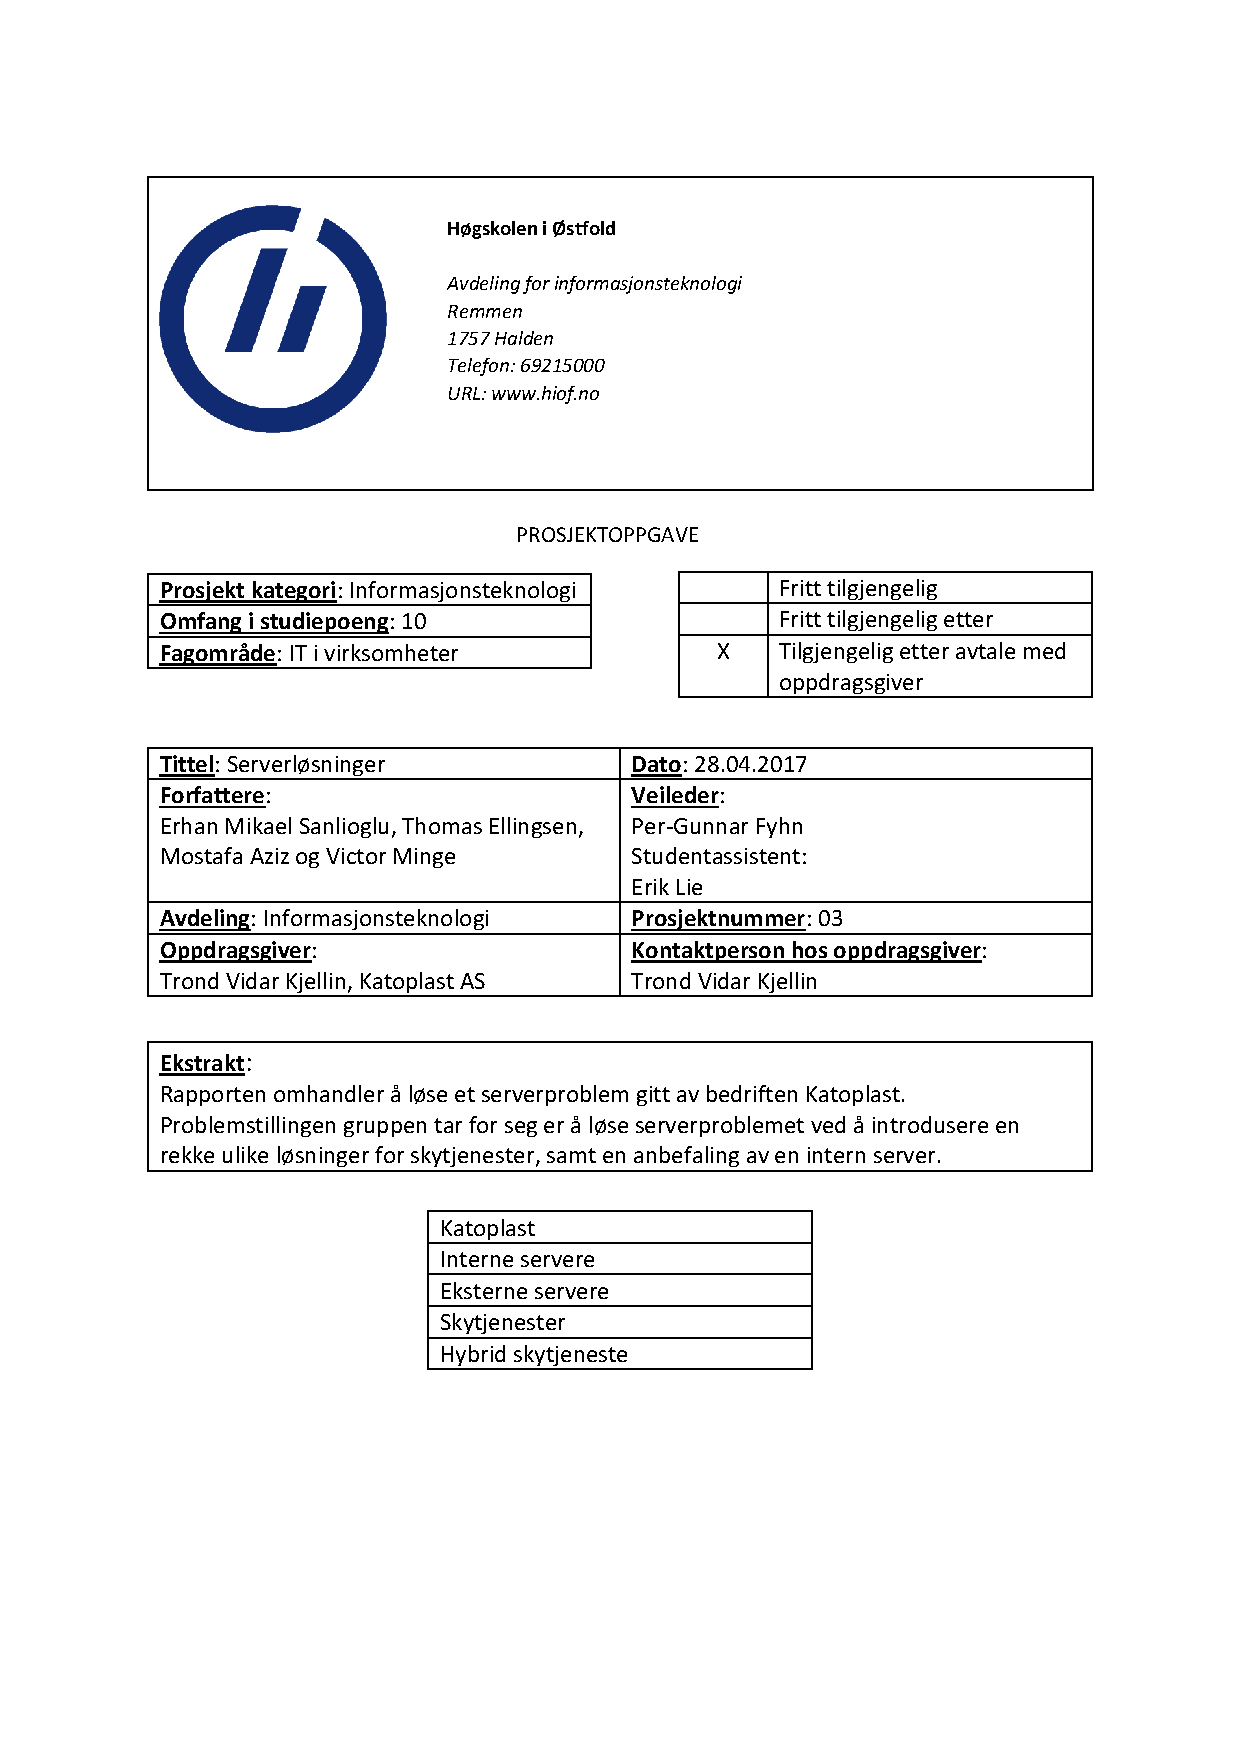
\includepdf{prosjektgruppe.pdf}

\addcontentsline{toc}{section}{Forord}
{\flushleft
\section*{Takk til}
% Hvorfor ble denne rapporten laget?
% Hva fikk dere til å jobbe med den?
% Hva slags type rapport kan leseren forventes å lese?
% Hvordan var reisen fra start til slutt?
% Skriv det på to paragrafer 2x85 ord ca. 1000 bokstaver:

\paragraph{} Vi ønsker å takke Trond Vidar Kjellin og Katoplast AS for å gi oss muligheten til å gjennomføre et interessant og viktig prosjekt som vil være relevant for fremtiden. Mulighetene og ressursene vi har hatt tilgang til har gitt oss en god start på arbeidslivet og hvordan det er å arbeide med et prosjekt innenfor en bedrift.

\paragraph{} Samtidig ønsker vi å rette en takk til vår foreleser Per-Gunnar Fyhn, og ikke minst vår studentassistent som har hjulpet og veiledet oss gjennom hele prosjektet. De har vært viktige støttepartnere for prosjektet vårt og for den avsluttende rapporten som skal leveres inn.

\addcontentsline{toc}{section}{Sammendrag}
\section*{Sammendrag} %Hold dere under 250 ord (dette er 424)
\paragraph{}Prosjektets formål er å presentere, analysere og beskrive forskjellige løsninger som kan hjelpe bedriften Katoplast AS med deres interne serverproblem. Rapporten vår vil ta for seg utfordringen ved å utarbeide løsninger som er fremtidsrettet, billige og ikke minst brukbare for bedriften. Rapporten inneholder en kartlegging av forskjellige løsninger og begrunnelser for hvilke av disse bedriften bør legge sitt fokus på. Rapporten inneholder en detaljert analyse av den nåværende situasjon, samt analyser og beskrivelser av de ulike mulighetene som kan være relevante for den endelige løsningen. Analysene vil legge vekt på å presentere ulike sider ved de ulike løsningene, fordeler og ulemper, og ikke minst hvordan hver løsning vil påvirke bedriften økonomisk. 

\paragraph{} Prosjektet vil ta for seg 3 muligheter som kan være aktuelle for bedriften. Gruppen vil fokusere på å presentere ulike sider ved å drifte egne servere, og benytte seg av eksterne løsninger. Prosjektet vil i tillegg presentere 2 hybrid-løsninger hvor data kan lagres både internt og i nettskyen, noe som vil forenkle en del av arbeidet for bedriften, men samtidig også holde det viktigste av informasjon innenfor bedriftens rammer. Hver og en av disse løsningene vil bli presentert opp mot ulike arbeidskrav som stilles, og ikke minst hvor mye de vil koste. Til slutt, vil gruppen presentere det endelige resultatet, en intern løsning, samt hvilken vei prosjektgruppen ville anbefalt bedriften å gå, dersom de skulle ønske å benytte seg av de mulighetene vi presenterer for dem. 



\include{Prechapter/takktill}


\renewcommand{\contentsname}{Innhold}
\tableofcontents
\listoffigures

\setcounter{page}{0}
\pagenumbering{arabic}

%%===========MAIN CONTENT============
\chapter{Introduksjon}
\paragraph{}I kapittel 1 ønsker gruppen å ta for seg en introduksjon av prosjektet. Dette er innledningen til selve oppgaven, og her beskrives hvem prosjektgruppen er, hvem oppdragsgiveren er, hva oppdraget er, hvilke forutsetninger og rammer prosjektet har og til slutt om strukturen på rapporten. Dette er et viktig kapittel for å få med seg informasjon om bedriften og prosjektgruppen og hvorfor prosjektet ble startet.
\section{Prosjektgruppen}
\paragraph{} Prosjektgruppen består av 4 medlemmer med ulik kompetanse og interesser. Den utgjør; Thomas Ellingsen, Erhan Sanlioglu, Mostafa Aziz og Victor Garberg Minge. Gruppen fant sammen etter å ha blitt kjent med hverandre under høstsemesteret og valgte å starte dette prosjektet sammen etter å ha snakket og diskutert sammen og kommet til enighet om at dette kan være en gruppe som kan utføre et godt prosjekt.


\begin{figure}[h]
\centering

\includegraphics[width=1.5in]{Bilder/victor2.jpg}

\includegraphics[width=1.5in]{Bilder/erhan2.jpg}
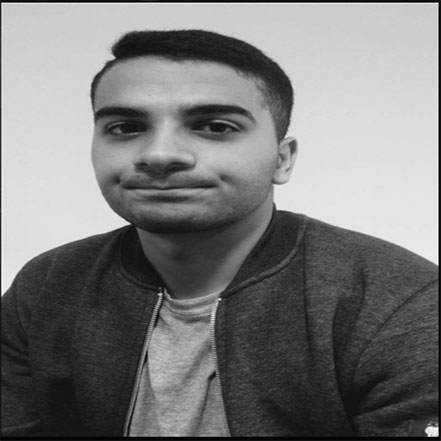
\includegraphics[width=1.5in]{Bilder/mosti2.jpg}

\includegraphics[width=1.5in]{Bilder/thomas2.jpg}
\end{figure}


\paragraph{} \textbf{Mostafa Aziz} er født den 01. november 1997, han valgte å studere informasjonssystemer på høgskolen i Østfold etter videregående skole. Mostafa har en rekke interesser deriblant datamaskiner og hvordan datamaskiner fungerer. Det å arbeide med servere var noe som interesserte Mostafa, ettersom det kunne være noe han kunne legge til som et område han kjenner til og ønsker å lære seg hvordan servere fungerer og hva som kan være relevant for fremtiden.




\paragraph{}\textbf{Thomas Ellingsen} født den 22.Juni 1995. Thomas har vært ett år i forsvaret og tatt utdanning som brannkostabel. I dag jobber han i Norskbrannvern hvor mesteparten av jobben går ut på kontroll og service av alarmanlegg. Thomas ønsker og kunne kombinere interessen for brann og redning med informasjonsteknologi. Derfor passet studiet informasjonssystemer på høgskolen i Østfold han perfekt. 

\paragraph{} \textbf{Victor Johannes Garberg Minge} er født den 04 August 1997. Victor studerer informasjonssystemer på Høgskolen i Østfold. Som ung har Victor alltid hatt stor interesse for det teknologiske, blandet med kreativitet falt han for linjen han nå går på Høgskolen. Victor har også en interesse for å løse problemer, noe som gjør IT et spennende område å arbeide og finne kreative løsninger. Som plan har Victor tenkt til å gjøre ferdig sin Bachelor på Høgskolen for å så se ann om videreutdanning eller arbeidslivet. Ellers har Victor en kjæreste og andre interesser deriblant idretten boksing og dataspill.

\paragraph{} \textbf{Erhan Mikael Sanlioglu} er født den 08 Desember 1994. Erhan studerer informasjonssystemer på høgskolen i Østfold. Med avlagt fagprøve og endt førstegangstjeneste kunne Erhan sette i gang med sine IT-studier på høgskolen. Erhan har hatt stor interesse for data i en tidlig alder og bestemte seg ganske tidlig for å ta en utdanning i dette feltet. Som fagarbeider har Erhan både arbeidserfaring fra det offentlige sektor og kunnskapen som trengs i dette fagfeltet. En kombinasjon som fagarbeider og en mastergrad i IT vil sikre fremtiden hans.

\section{Oppdragsgiver}

\begin{figure}[H]
\centering

\includegraphics[width=3.5in]{Bilder/katoplast_logo.png}
\caption{Katoplast logo}
\end{figure}


\paragraph{} Oppdragsgiver for prosjektet er daglig leder ved Katoplast AS, Trond Vidar Kjellin som har tillat en gruppe med studenter fra Høgskolen i Østfold å utføre et prosjekt i bedriften Katoplast AS.

\paragraph{} Bedriften ble grunnlagt i 1972 av Gunnar og Ivar kjellin. Bedriften driver produksjon, utforming, konstruksjon og materialvalg av plastprodukter. Plastproduksjonen skjer gjennom 3D-printing og gjennom støping av former. Katoplast har om lag 15-20 ansatte og selve produksjonen blir driftet av 14 forskjellige maskiner. \footnote{http://www.katoplast.no/produkter/}.

\paragraph{}Virksomheten har med årene flyttet flere ganger. I 1983 ble beslutningen tatt om å bygge egne lokaler i Tistedal, og disse var innflytningsklare på høsten 1984. Etter dette har det vært behov for flere utbygginger.\footnote{http://www.katoplast.no/om-katoplast/}.

\section{Oppdraget}
\paragraph{} Som oppdrag har prosjektgruppen blitt utdelt en rekke problemstillinger som gruppen skulle ha som utgangspunkt. Disse problemstillingene inkluderte alt fra å løse små, administrative oppgaver, til å finne store løsninger knyttet til ERP-system. Disse oppgavene inkluderte blant annet oppdatering av serverne, mye manuelt arbeid når det gjelder å legge inn data om kjøp og salg som har blitt gjort og annen informasjon om produkter og kunder.  I midlertid, valgte gruppen å gå for å løse serverproblemet som preger bedriften i stor grad. Oppdraget vil ta for seg flere, forskjellige sider ved ulike serverløsninger som kan være aktuelle for bedriften Katoplast AS

\paragraph{} I løpet av året 2016 har Katoplast opplevd problemer med sine servere, og hvordan deres IT-systemer generelt fungerer. Bedriften presenterte en rekke problemstillinger for gruppen som var IT-relaterte, og som gjorde at arbeidet deres i bedriften ikke ble gjort effektivt nok. Mye av problemene inkluderte høye kostnader, trege servere og manuelt arbeid som krever mye tid. Bedriften benytter seg av to ERP-system som tar for seg en rekke oppgaver innen bedriften. Access-løsningen tar seg av oppgaver knyttet til produksjonsdataen, mens en Mamut-løsning tar seg av det økonomiske regnskapet som gjennomføres. I midlertid, krever disse ERP-systemene at mye av arbeidet gjøres manuelt og dette viser seg å være et problem. Dette krever mye tid og arbeidskraft og dette fører til at mye av hovedfokuset rettes mot IT-oppgavene fremfor produseringen av varer til kunder.

\paragraph{}Gruppen diskuterte de ulike problemstillingene som ble presentert av bedriften, og som konklusjon ble resultatet å forsøke å rette, eller hjelpe Katoplast med å finne en løsning for deres serverproblem. Problemstillingene hadde et stort omfang og det var dermed rimelig å velge å fokusere på kun et av problemene fremfor alle.

\paragraph{}Situasjonen i bedriften når det gjelder servere, er at de nåværende serverne begynner å bli gamle og trege, og ikke minst skaper de problemer og utsettelser for bedriften. Prosjektets hovedfokus vil dermed legges på dette med servere og det å analysere og finne en løsning som kan være aktuell for bedriften. Katoplast ønsker en løsning som legger vekt på brukervennlighet, funksjonalitet, riktig mengde med datalagring og ikke minst en rimelig pris som kan lette på det økonomiske trykket som bedriften opplever. Gruppen må også legge vekt på fremtiden og hva som kan være enklest å håndtere for bedriften.

\begin{figure}[H]
\centering
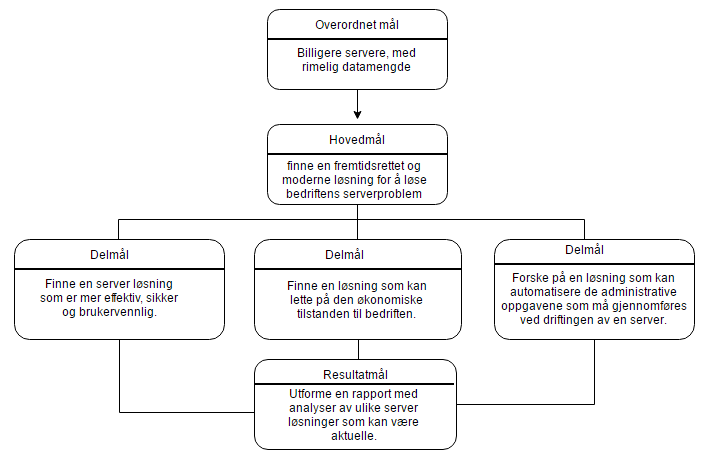
\includegraphics[width=6.5in]{Bilder/maal.PNG}
\caption{Prosjektets mål og resultatkrav}
\end{figure}

\section{Forutsetninger og rammer}

\paragraph{}Katoplast AS var åpne for at prosjektet og gruppen kunne ta fatt på oppgaven fra flere ulike vinkler, uten for mange avgrensninger og rammer som kunne eventuelt hindre sluttrapporten å oppnå beste kvalitet. Prosjekteierne ønsket ikke å begrense gruppen for mye og fokuserte hovedsakelig kun på noen små avgrensninger, som prosjektet måtte forholde seg til. Dette er svært positivt for gruppen ettersom det vil bli lettere å utforme analyser av ulike serverløsninger som kan være aktuelle for bedriften å velge. Flere muligheter vil bli dekket, og Katoplast vil kunne ha et større utvalg av løsninger når de til slutt skal velge den veien de ønsker å gå for. Katoplast var mest foukserte på sikkerhet, og var usikre når det gjaldt sky-løsninger. 

\section{Rapportstruktur}
\paragraph{} Prosjektet er delt opp i flere kapitler som tar for seg ulike områder for å skape en helhetlig rapport som er detaljert, men samtidig  enkel å forstå. Kapittel 1 av rapporten vår tar for seg introduksjonen av prosjektet. Her presenterer gruppen seg selv, oppdragsgiveren, hva oppdraget er og hva vi ønsker å oppnå og hvilke forutsetninger som er satt for prosjektet.

\paragraph{} Det neste kapittelet, kapittel 2, tar for seg teori og ulik fagstoff for prosjektet. Her beskrives vanskelig terminologi, og ulike konsepter som er viktig å forstå og vite hva er før en går videre med å lese prosjektet. Kapittel 2 er viktig for å skape et forståelig bilde av hele rapporten og de ulike analysene som er blitt gjort. Det vil finnes mange vanskelige begreper og uttrykk og teori kapittelet vil være til god hjelp for å forstå disse. I dette kapittelet beskrives de ulike delene ved servere og nettskyer, og de ulike tjenestene forklares.

\paragraph{} Det tredje kapittelet tar for seg metode. Altså hvilke metoder som ble benyttet for å finne frem til informasjon og hente ut informasjon. Den tar for seg de ulike metodene som gruppen benyttet, fra intervju til nettsøk til spørreundersøkelser. Den inkluderer også en situasjonsanalyse av bedriften for å få et bedre bilde av hvilken situasjon bedriften befinner seg i. Situasjonsanalysen er viktig for metode, ettersom den er viktig for innhentingen av informasjon for de senere analysene.

\paragraph{} Det fjerde kapittelet tar for seg de mange resultatene som gruppen har kommet til etter å ha gjennomført metodene, og med en situasjonsanalyse i bakhode. Her tar prosjektet for seg en arbeidskravsanalyse for å forstå hva som bør legges vekt på i analysene av de ulike løsningene, samt de mange resultatene som følge av forskningen som ble gjort på de ulike løsningene som gruppen har valgt å fokusere på. Her finner man resultatene av spørreundersøkelsen og et diagram som viser prisen på de ulike løsningene. 

\paragraph{} Kapittel 5 er diskusjonsdelen og diskuterer de ulike løsningene opp mot arbeidskravsanalysen og situasjonsanalysen som har blitt dannet. Diskusjons delen tar for seg de ulike løsningene for interne servere, sky tjenester og hybride løsninger som er viktige for Katoplast å vite. Dette er den viktigste delen av prosjektet ettersom den tar for seg hvordan de ulike løsningene kan påvirke Katoplast sin situasjon, og hvilken pris hver og en av de har.

\paragraph{} Avslutningsvis, så kommer konklusjonen som er det sjette og siste kapittelet. Konklusjonen tar for seg avslutningen på rapporten og vil komme med en anbefaling på hvilken løsning prosjektgruppen mener er den beste for bedriften Katoplast. Konklusjonen vil oppsummere hele prosjektet og prosjektgruppen vil ta et valg ut i fra den forskningen og de resultatene som gruppen har samlet sammen. 
\footnote{https://wiki.hiof.no/index.php/Bacheloroppgaven}
\chapter{Teori}
\paragraph{} Dette kapittelet vil gå dypere inn på den teoretiske delen rundt selve oppgaven. Her beskrives de grunnleggende elementene som benyttes i prosjektet, hva de betyr og hvordan de fungerer. I tillegg blir ulik terminologi som benyttes i rapporten forklart her og det er dermed nødvendig å lese og forstå denne delen før en fortsetter med å lese rapporten. Med dette ønsker gruppen å øke forståelsen til leseren og danne et bedre grunnlag for de som leser rapporten. Dette vil hjelpe med å velge den beste løsningen for bedriften.
\section{Grunnleggende elementer}
\paragraph{Hva er en server?} 
En server er et datamaskinprogram som forsørger forskjellige tjenester til forskjellige programmer og deres brukere. Datamaskinen serverprogrammet kjører på refereres til som en “server”. Servere deles ofte inn i forskjellige kategorier basert på hvordan de brukes, f.eks. en “Web Server” \footnote{http://whatis.techtarget.com/definition/server}

\paragraph{Hva er en nettsky?}  

En fremtidsrettet teknologi hvor data og informasjon lagres på servere som ligger på eksterne steder som er tilknyttet internett Nettskyen tillater brukere å lagre informasjon uten å behøve å selv drifte en egen server. Microsoft, Google, og Amazon. Nettskybasert databehandling tilbyr en rekke fordeler for fortetninger og brukere. Vi kan dele fordelene inn i 3 forskjellige grupperinger.\footnote{https://no.wikipedia.org/wiki/Nettskyen}.

\paragraph{Hva er en hybridløsning?} 

En hybrid-løsning i prosjektet handler om å finne en mulig vei for bedriften med blandede løsninger som kan være aktuelt å bruke. For eksempel, å bruke både interne servere som blir plassert hos bedriften og en liten cloud-løsning som befinner seg hos en annen leverandør.
Dette er noe som kan være aktuelt hvis bedriften ønsker å ha noe av dataene sine på huset.\footnote{http://www.dummies.com/programming/cloud-computing/hybrid-cloud/what-is-hybrid-cloud-computing/}

\paragraph{} Nettskyen, skyen eller cloud er en fellesbetegnelse på alt fra dataprosessering og datalagring til programvare på eksterne servere tilknyttet Internett. (En server er en programvare som tilbyr en eller flere tjenester over et datanettverk. Begrepet server, eller tjener på norsk er også ofte brukt på maskinvaren som programmet/programmene kjøres fra, så lenge maskinen har kapasiteten til å utføre oppgavene.

Vi kan også dele skytjenestene opp i forskjellige leveransemodeller. Da går det altså hovedsakelig ut på allmenn tilgjengelig {\small (Public Cloud)}, privat tilgjengelig {\small (Private Cloud)} og sist hybridsky {\small (Hybrid Cloud)};\par
\begin{description}[noitemsep]
\item[Public Cloud] En allmenn tilgjengelig sky betyr at skytjeneste er gjort tilgjengelig for alle kunder av leverandøren.
\item[Private Cloud] Privat tilgjengelig sky betyr at skytjenesten er gjort privat, og dedikert kun til en gruppe av kunder. Skytjenesten gjelder altså kun for virksomheten den er dedikert til. Som vi ser, her vil skyen typisk bli dedikert til den enkelte kunden eller den definerte kundegruppen. Denne løsningen åpner for en større grad av spesifikke tilpasninger.
\item[Hybrid Cloud] Hybrid sky er altså en blanding av tjenestene som kan leveres ovenfor. En god blanding av de begge.
\end{description}
\begin{figure}[H]
\centering
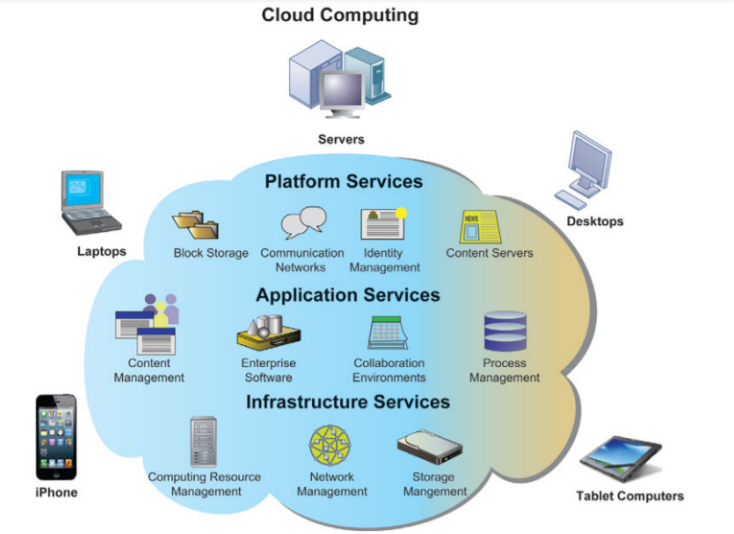
\includegraphics[width=6.5in]{Bilder/cc.PNG}
\caption{En visuell representasjon av hvordan Sky tjenester er satt opp.(Laudon \& Laudon, 2016, s.223)}
\end{figure}

Som vi kan lese ovenfor, tilbyr skybaserte løsninger en rekke forskjellige modeller. Disse modellene er veldig fleksible, brukervennlige og tilpasset behov. Under vil du finne ulike skytjenester som tilbys fra bedrifter som Microsoft, Amazon og Google:
\begin{description}
\item Microsoft Azure er en skytjeneste som er utviklet av Microsoft og som tilbyr brukere av tjenesten en rekke verktøy og programmer knyttet til lagring, utvikling og distribuering av informasjon og data.\footnote{https://azure.microsoft.com/nb-no/}

\item Amazon Web Services (AWS) er Amazon sitt svar på en skytjeneste. Med Amazon AWS har man tilgang til en rekke funksjoner, deriblant muligheten til å enkelt lagre store og små datamengder, levere ulikt innhold til brukere og kraftige maskiner som tar seg av mye av arbeidet.\footnote{https://aws.amazon.com/about-aws/}

\item Google Disk er en versjon av en Sky tjeneste forenklet så mye som mulig for å tilpasse så mange brukere som mulig. Med Google Disk har man tilgang til alle filene og mappene sine, uansett hvor man er, med et svært enkelt brukergrensesnitt og hvor mye av de administrative oppgavene blir tatt hånd om.\footnote{https://www.google.com/drive/}

\item Microsoft PowerShell er et komandolinjeskall for systemadministratorer. PowerShell fungerer i form av at systemadministrator skriver inn kommando for å styre operativsystemet til å utføre bestemte oppgaver. Det å arbeide i PowerShell kan få brukeren til å styre programmer og manipulerer elementer i systemets database. Når det er nevnt kreves det noe datakunnskaper for å utføre disse manipulasjonene. \footnote{http://www.datamaskin.biz/Systems/windows/212342.html}
\end{description}

\section{Server}
\paragraph{} En server er et datamaskinprogram som forsørger forskjellige tjenester til forskjellige programmer og deres brukere. Datamaskinen serverprogrammet kjører på refereres til som en “server”. Servere deles ofte inn i forskjellige kategorier basert på hvordan de brukes, f.eks. en “Web Server” \todo[author=Ole]{{\scriptsize Bruk heller enquotes}} 
\begin{figure}[H]
\centering
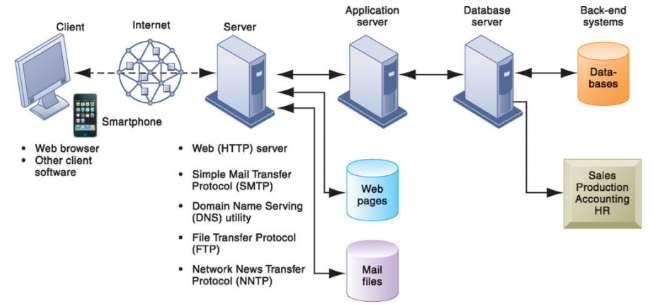
\includegraphics[width=6.5in]{Bilder/cc2.PNG}
\caption{En modell som viser en visuell forklaring på hvordan datamaskiner, Internet og servere henger sammen med andre systemer. (Laudon \& Laudon, 2016, s.305) }
%\todo[inline,author=Ole]{{\scriptsize Dere må ref'e til hvor dette bildet er tatt fra. Ved å linke til bibliografien deres. Dette må dere gjøre med ALLE bilder og grafikk dere har hentet fra andre kilder en dere selv. Dette gjør dere ved å bruke \textbackslash cite\{labeltype:refname\}}}
\end{figure}

\section{Terminologi}
\paragraph{} {\bfseries Interne servere:} Interne servere i en bedrift vil si at serveren står fysisk i lokalene til selskapet. Disse serveren vil altså lagre data, kjøre applikasjoner og holde på forskjellige API/ERP løsninger som selskapet benytter. \footnote{https://no.wikipedia.org/wiki/Server}
\footnote{http://whatis.techtarget.com/definition/server}

\paragraph{} {\bfseries ERP:} Enterprise resource planning (ERP) er en programvare som støtter flere av en bedrifts virksomgetsområder,  som produksjon, lager, salg , innkjøp og økonomi.  Målet med ERP er å håndtere virksomgetens informasjon.
\footnote{https://www.oracle.com/applications/erp/what-is-erp.html}

\paragraph{} {\bfseries Operativsystem:} Et operativsystem (OS) er den grunnleggende programvaren på en datamaskin, og det som tildeler de forskjellige ressursene i datamaskinen til andre programmer.
\footnote{https://no.wikipedia.org/wiki/Operativsystem}

\paragraph{} {\bfseries PaaS(Platform as a service):}  Plattform som en tjeneste eller applikasjonsplattform som en tjeneste (aPaaS) er en kategori av cloud 
computing-tjenester som gir en plattform som gjør det mulig for kunder å utvikle, kjøre og administrere applikasjoner 
uten kompleksiteten i å bygge og vedlikeholde infrastrukturen som vanligvis er knyttet til å utvikle Og lanserer en app.
\footnote{https://en.wikipedia.org/wiki/Platform\_as\_a\_service}

\paragraph{} {\bfseries IaaS(Infrastructure as a Service):} Infrastruktur som en tjeneste er en form for cloud computing som gir databehandlings ressurser over Internett.
\footnote{http://searchcloudcomputing.techtarget.com/definition/Infrastructure-as-a-Service-IaaS}

\paragraph{} {\bfseries SaaS(Software as a Service):} Programvare som en tjeneste er en programvaredistribusjonsmodell 
der en tredjepartsleverandør er vert for programmer og gjør dem tilgjengelige for kunder over Internett.
\footnote{http://searchcloudcomputing.techtarget.com/definition/Software-as-a-Service}

\paragraph{} {\bfseries Data:} Informasjon, brukes for grunnlag av begrynnelse, diskusjon eller beregninger. 
\footnote{https://www.merriam-webster.com/dictionary/data}

\paragraph{} {\bfseries API:} Application Programming Interface, er et programfunksjon som lar brukeren koble sammen flere programmer.  Man kan da utveksle informasjon på tvers av programmene. 
\footnote{}
\paragraph{} {\bfseries Programvare:} Programvare (engelsk: software) er en fellesbetegnelse på dataprogrammer. Alt som er digitalt i dag har en form for programvare. 
\footnote{http://www.computerhope.com/jargon/s/software.htm}

\paragraph{} {\bfseries Maskinvare:} Maskinvare er de fysiske delene en server/datamaskin består av.
\footnote{http://www.computerhope.com/jargon/h/hardware.htm}
\footnote{http://www.computerhope.com/issues/ch000039.htm}

\paragraph{} {\bfseries Skytjenste (Cloud):} En Skytjeneste (Cloud) er et sett med applikasjoner, tjenester, lagring og maskinvare som opprettholdes og driftes av en tredje-part, som tillater andre bedrifter og organisasjoner å enkelt kunne lagre data og informasjon, uten å måtte bry seg om det tunge, administrative arbeidet som må gjøres for å drifte en slik løsning. Skytjenestene tillater brukere å lagre informasjon og data på en server som befinner seg på et eksternt sted på internett for å gjøre det så enkelt som mulig for brukeren.
\footnote{https://www.datatilsynet.no/Teknologi/Skytjenester---Cloud-Computing/Hva-er-nettskytjenester/}
\footnote{https://www.anskaffelser.no/it/temaer-it/skytjenester-cloud}

\paragraph{} {\bfseries Hybrid Cloud:} En "Hybrid Cloud" eller en hybrid skytjeneste, er en form for Skytjeneste som kombinerer og blander tjenestene og egenskapene fra de grunnleggende formene for nettskyer, Public og Private cloud og tilbyr brukerne å benytte seg av en blanding av disse for å oppnå et enhetlig, sikkert og automatisert lagrings system for både viktig og mindre viktig data og informasjon innenfor bedriften.
\footnote{https://www.microsoft.com/nb-no/cloud-platform/hybrid-cloud}

\paragraph{} {\bfseries SSD:} Solid State Drive (SSD) er en nyere form for harddisk (maskinvare) som benyttes som et lagringsmedium hvor søketiden og lagringen foregår med høyere hastighet enn med en vanlig harddisk. Som følge av den kjappere lagringen som en SSD kan gjennomføre, koster også disse harddiskene mer enn de vanlige harddiskene.
\footnote{https://www.komplett.no/category/10088/datautstyr/lagring/harddisker/ssd}
\footnote{http://uk.pcmag.com/storage-devices-reviews/8061/feature/ssd-vs-hdd-whats-the-difference}

\paragraph{} {\bfseries HDD:} Hard Disk Drive (HDD) er den tradisjonelle formen for en harddisk og er et lagringsmedium som er tilstrekkelig brukt i verden. Slike tradisjonelle harddisker har ofte en rekke ulemper ved seg, blant annet at de er sårbare og ikke minst tregere med å gjennomføre lagring enn nyere harddisker.
\footnote{http://uk.pcmag.com/storage-devices-reviews/8061/feature/ssd-vs-hdd-whats-the-difference}


\paragraph{} {\bfseries iSCSI:} Internet Small Computer Systems Interface (iSCSI) er en internet protokoll som står for den lagringen som gjennomføres over internett. iSCSI håndterer lagringen av data over internett, hvor det ikke er noen begrensning på avstander. Store organisasjoner benytter seg av denne protokollen hvor de tar imot informasjon og data fra andre brukere og lagrer disse i store datasentre. Kundene kan dermed gjennomføre lagring uten behov for fysiske harddisker.
\footnote{https://no.wikipedia.org/wiki/ISCSI}

\paragraph{} {\bfseries DDOS-angrep:} Et DDOS-angrep (distribuert tjenestenekt) er en form for Internett angrep hvor maskinene til et offer angripes og hvor brukeren, som blir angrepet, hindres i å gjennomføre handlinger eller få tilgang til informasjon. Dette kjennetegnes ofte ved man mister Internet tilgang. Dette kan føre til stor nedetid og koste dyrt for de som angripes.
\footnote{http://www.digitalattackmap.com/understanding-ddos/}
\footnote{https://no.wikipedia.org/wiki/Tjenestenektangrep}

\paragraph{} {\bfseries Ulovlig Hacking:} Ulovlig Hacking er en form for datakriminalitet hvor en person benytter sine ferdigheter, programmer og løsninger for å bryte seg inn og ulovlig hente informasjon eller manipulere data hos andre personer eller bedrifter. Dette kan føre til store konsekvenser for de som blir utsatt hvor sensitive opplysninger kan bli lekket. 
\footnote{https://snl.no/hacker}

\paragraph{} {\bfseries Nano Server:} Nano Server er et helt nytt og fremtidig konsept som er utviklet av Microsoft og som gir deg muligheten til å fjernstyre operativsystemene til en windows server og som er optimalisert for skytjenester. Fordelen med dette er at den tar opp svært lite plass, er merkbart raskere og behøver mindre oppdateringer enn de tradisjonelle serverne.
\footnote{https://www.pluralsight.com/blog/it-ops/microsoft-nano-server-announced}
\footnote{https://technet.microsoft.com/en-us/windows-server-docs/get-started/getting-started-with-nano-server}

\paragraph{} {\bfseries OpenStack:} OpenStack er programvare som benyttes av leverandører av nettskyer hvor alle ressursene knyttet til programvaren er frie og åpne til allmennheten slik at de kan benyttes og endres på akkurat slik man ønsker. Dette tillater for nye ideer og metoder for nettskyer.
\footnote{https://www.openstack.org/}

\paragraph{} {\bfseries OpenSource:} Programvare som har OpenSource-lisens er programvare som tillater andre personer å endre, manipulere og distribuere programvaren akkurat som de ønsker uten at dette skal få noen konsekvenser. Dette åpner for store muligheter for både brukere og utviklere.
\footnote{https://opensource.com/resources/what-open-source}

\paragraph{} {\bfseries Virtuell maskiner:} En virtuell maskin er en programvare-simulering av en komplett datamaskin som utfører programmer på samme måte som en fysisk datamaskin. Med en slik fysisk maskin kan man kjøre simulering av flere maskiner, også med ulike operativsystemer. Hvis en benytter Windows 7 som hovedoperativsystem, men er avhengig av en virtuell maskin med Windows 10 på grunn av et program man er avhengig av i jobbsammenheng- kan man bare bytte om på operativsystemet sitt ved hjelp av en slik maskin. \footnote{https://it.uib.no/Virtuell\_maskin}

\chapter{Metode}
\paragraph{}I kapittel 3 dreier det seg om metode. Med metode menes hvilke arbeidsmåter som er tatt i bruk for innhentingen av informasjon. I dette tilfellet inkluderer dette nettsøk, intervju og en spørreundersøkelse. Metode beskriver hva gruppen gjorde for å finne den informasjonen som blir benyttet for å skape en troverdig rapport.
\section{Innhenting av informasjon}
\paragraph{} \gruppen arbeidet med oppgaven på en rekke ulike måter for å finne informasjon og data for løsningene og analysene. Innsamlingen av informasjon foregikk på flere måter, for det første så arrangerte gruppen 2 møter med daglig leder for Katoplast for å innhente så mye informasjon som mulig før gruppen gikk i gang med prosjektet. Under disse møtene med Katoplast, dokumenterte gruppen det viktigste av informasjon, samt også hva det er bedriften ser etter i rapporten og de løsningene rapporten skal fremstille som konklusjon.

\paragraph{} I tillegg til å gjennomføre møter med Katoplast, var det også betydelig å gjennomføre flere, grundige søk på internett og i bøker for å finne de mest optimale løsningene og det viktigste av informasjon som kreves for å skrive gode analyser. Innhentingen av informasjon ble delt i 4, hvor hvert gruppemedlem fikk et tema de skulle fokusere på når de skulle hente ut informasjon. Informasjonsinnhentingen krevde samtidig at kildene som ble gjennomsøkt var troverdige og at disse ble analysert og sammenlignet med andre kilder for å finne korrekt og troverdig informasjon. 

\paragraph{} En rekke informasjon lå i tidligere dokumenter fra faget "Webutvikling" hvor gruppen allerede hadde notert troverdig og verdifull informasjon om servere og Sky løsninger. I disse dokumentene var det også rikelig med informasjon rundt terminologi og hvordan internett vil utvikle seg fremover. Dette er informasjon som kan være vesentlig for prosjektet og analysene å ha med, og dermed ble denne informasjonen også inkludert i prosjektet.

\paragraph{} I tillegg til dette, valgte gruppen å sende et dokument med en rekke spørsmål til daglig leder av Katoplast, Trond Kjellin, slik at han kunne svare på noen få spørsmål som gruppen lurte på. Dette var en rekke spørsmål som ville hjelpe gruppen med å rangere  hvilke funksjoner og deler ved løsningene som skulle velges, og hvilke deler ved analysene det skulle legges mer vekt på enn andre. Samtidig var disse spørsmålene også vesentlige for at gruppen kunne utvikle en situasjonsanalyse av den nåværende situasjonen og problemene som bedriften opplever. 

\section{Intervju}
\paragraph{} Gruppen oppsøkte Katoplast via e-post og ønsket å sette opp et intervju. 10.02.2017 hadde prosjektgruppen det første møte med bedriften. Gruppen hadde en velkomstrunde i bedriften og fikk kartlagt hvordan bedriften jobber daglig. Det første møte med bedriften gikk ut på å finne ut av hva gruppen kunne bistå med for Katoplast. Etter endt møte sto prosjektgruppen igjen med problemstillinger som ERP, administrative oppgaver og servere. Det første intervjuet ga gruppen et bredt spekter av problemer som gruppen kunne ta for seg. Gruppen valgte å fokusere på å hjelpe bedriften med deres server problemer for å kutte ned på prosjektet. Dette var viktig med tanke på tidsrommet og hvilke ressurser gruppen hadde tilgang til.

\paragraph{} På det neste møte med daglig leder Kjellin, var det vesentlig for gruppen å kartlegge Katoplast sin server situasjon i dag, hva slags problemer de opplever, både interne og eksterne, og ikke minst finne ut av hva Katoplast ønsker å oppnå med prosjektet. Dette intervjuet var avgjørende for at gruppen kunne begrense arbeidet til mindre løsninger, fremfor å skrive en bred analyse om mange løsninger.

\section{Nettsøk}
\paragraph{} Som nevnt tidligere, så delte gruppen  opp nettsøket i 4 deler; Interne servere, eksterne servere, Cloud og Hybrid-løsning. Hvert gruppemedlem fikk tildelt hver sin del av disse 4 delene, og internett søket ble satt i gang når medlemmene var klare.

\paragraph{} For interne servere gjennomførte prosjektgruppen en rekke søk på nettet hvor gruppen la vekt på norske leverandører av servere. Det var nødvendig å finne leverandører som hadde akseptable priser, og ikke minst god service slik at det ville være enklere å få ut informasjon.

\paragraph{} For Hybride-løsninger ble det først og fremst søkt gjennom hvilke leverandører som tilbyr en Hybrid Cloud, og hvilke av disse leverandørene som virker mest troverdige. Gruppen benyttet ulike nettsider for å finne den beste informasjonen. Gruppen gikk gjennom en rekke med anmeldelser og sammenligninger av ulike hybride løsninger og hvordan disse fungerte sammen. Den mest fundamentale ressursen for informasjon var leverandørenes egne nettsider og informasjon. Det var her gruppen fant beste kvalitet på informasjonen og ikke minst var det troverdig informasjon. 



\chapter{Resultat}
\paragraph{} Kapittel 4 handler om resultatene fra kapittel-3. Dette kapittelet tar for seg de resultatene som er kommet som følge av gruppens forskning. Her presenteres de ulike resultatene som er funnet samt en arbeidskravs- og en situasjonsanalyse som hjelper prosjektgruppen med å bedre kartlegge det som kreves for å fikse problemet til katoplast.

\section{Arbeidskravsanalyse} 
\paragraph{} Ut i fra informasjonen gruppen hadde tilegnet seg fra Katoplast, utarbeidet prosjektgruppen en arbeidskravsanalyse som skulle ta for seg de viktigste elementene ved en server løsning for å finne den beste løsningen for Katoplast. Gruppen tok for seg en rekke elementer som bedriften satte vekt på, og hvorvidt disse ulike elementene skulle spille inn på hvilke løsninger som skulle analyseres.

\paragraph{}\textbf{Arbeidskravsanalyse som gruppen kom frem til. }
\begin{figure}[H]
\centering
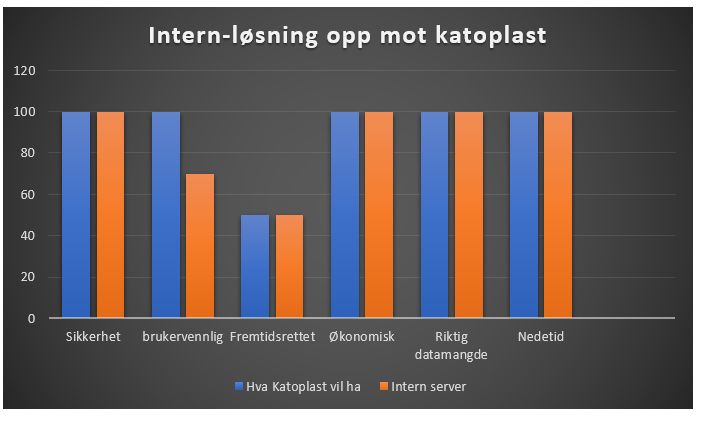
\includegraphics[width=5.5in]{Bilder/abc.PNG}
\caption{Arbeidskravsanalyse}
\end{figure}


\paragraph{Sikkerhet:} \hspace{-0.95em} Sikkerheten til katoplast er det mest fundamentale for bedriften. Bedriften holder på store mengder med sensitiv data som de ønsker å holde hemmelig. Generelt er bedriften avhengig av riktig data for at en normal arbeidsdag skal kunne gå som planlagt. Dersom noe av den sensitive dataen skulle komme på avveie kan bedriften i verste fall gå konkurs. Derfor er sikkerheten på serverløsningene noe av det viktigste og dermed også det gruppen la størst vekt på når de forskjellige løsningene ble analysert. Det er vesentlig at leverandørene tilbyr beskyttelse mot hackere og DDOS-angrep for å unngå nedetid og at sensitiv data ikke skal bli kompromittert. 
\footnote{https://nettvett.no/ddos-angrep/}

\paragraph{}{\bfseries Brukervennlighet:} \hspace{-0.95em}  Det er vesentlig for bedriften å kunne bruke serverne slik de skal brukes. I dag er det dagligleder som står for det meste av drifting og oppdatering av egen server. Dette er oppgaver som daglig leder ønsker å unngå. Det er essensielt at en serverløsning er komfortabel å benytte seg av og tillater enkle metoder for lagring og henting av informasjon og data. Det er også et stort pluss at løsningen tar seg av en rekke administrative oppgaver som ofte krever tid og arbeid når de må gjøres manuelt.  


\paragraph{}{\bfseries Framtidsrettet:} \hspace{-0.95em} Dette kravet tar for seg hvorvidt løsningen er framtidsrettet. Det er nødvendig å tenke om løsningene kan brukes igjennom flere år. Dette kan man tjene på økonomisk. Løsningen til Katoplast i dag er ikke like fremtidsrettet som andre løsninger. Interne servere har blitt brukt i lang tid og vil mest sannsynlig fortsette å brukes i lengre tid fremover, men det er likevel slik at en bør ha et fremtidsrettet syn når det kommer til løsningene. Dette kan lette på det økonomiske trykket og tidspresset som preger katoplast. I midlertid, ønsker ikke bedriften å sette dette kravet for langt oppe på listen og vil nøye seg med en mindre fremtidsrettet løsningen.

\paragraph{}{\bfseries Økonomisk:} \hspace{-0.95em} Økonomisk planlegging og styring er avgjørende i en bedrift. Derfor har gruppen valgt å legge økonomi som et arbeidskrav for løsningen. Det er vesentlig at de ulike serverløsningene som presenteres og analyseres er rimelige når det gjelder pris. Det er vesentlig at kvaliteten på løsningene er høyt, men samtidig hjelper det stort at løsningen ikke er for kostbare. Bedriften er en relativ liten bedrift og har ikke utallige med krav til for avanserte og dyre løsninger.

\paragraph{}{\bfseries Datamengde:} \hspace{-0.95em} Datamengden til bedriften ligger i dag på 500GB. Dette er data de har samlet siden 1972. For at prosjektet skal kunne finne den beste løsningen må man tenke igjennom dataforbruket til bedriften. Ved å finne den riktige datamengden kan dette lette på det økonomiske trykket for bedriften, og samtidig gjøre arbeidet for å finne en løsning lettere for gruppen. 

\paragraph{}{\bfseries Nedetid:} \hspace{-0.95em} For Katoplast var det viktig at deres servere er oppe og kjører hele tiden. De ønsker en løsning hvor serverne har overbevisende sikkerhet til å motstå feil eller andre problemer som kan eventuelt føre til nedetid. Dersom serverne skulle gå ned i lengre tid kan følgene bli katastrofale for katoplast. Bedriften har veldig sjeldent nedetid, derfor er det avgjørende at løsningen som gruppen kommer frem til kan vedlikeholdet dette.

\section{Situasjonsanalyse (SWOT-Analyse)}
\paragraph{} Før gruppen satte i gang arbeidet med å analysere ulike muligheter og løsninger, var det betydelig å ha en oversikt over hvilken situasjon bedriften befinner seg i nå og hva det er som er nødvendig å tenke på når gruppen søker etter informasjon for analysene. For å sikre prosjektet mot feilaktig informasjon, samt for å forstå hva det er Katoplast behøver utarbeide gruppen en detaljert situasjonsanalyse som tar for seg hvordan situasjonen i bedriften er fra i dag og hvordan den kan forbedres
\paragraph{} Med en slik Situasjonsanalyse vil gruppen ha bedre oversikt over situasjonen til bedriften, hvilke felter som kan påvirke løsningene og hvilke veier det er best å gå for å avklare problemer i katoplast sin situasjon i dag og finne den beste løsningen for bedriften. En oversiktlig analyse av situasjonen til katoplast i dag vil gjøre det lettere for gruppen å vurdere hvilke problemer som bør rettes opp i når de nye løsningene analyseres.

% jeg har laget en mal på en tabell (hvor jeg bruker longtable og booktabs for fremheve hvordan dere kan gå frem når dere bygger skikkelige tabeller. Alt nedenfor er kompilerbart i latex på en god måte.
% For å forstå dette bedre (ikke nå, det tar tid) så kan dere lese booktabs og longtable sine package documentation over på;
% http://ctan.uib.no/macros/latex/contrib/booktabs/booktabs.pdf
% http://mirrors.ctan.org/macros/latex/required/tools/longtable.pdf
%
% For nå, kan dere fylle inn resten av tabellen: (jeg har ikke tid.).
%
% ---Ole

%\paragraph{} %Flytt disse over i tabellen under:
%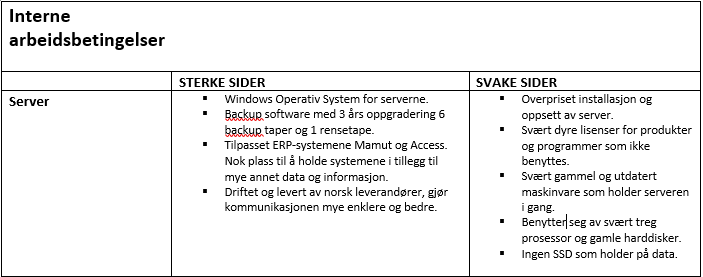
\includegraphics[width=\textwidth]{Bilder/s1.PNG}
%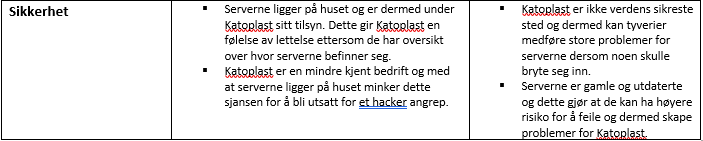
\includegraphics[width=\textwidth]{Bilder/s3.PNG}
%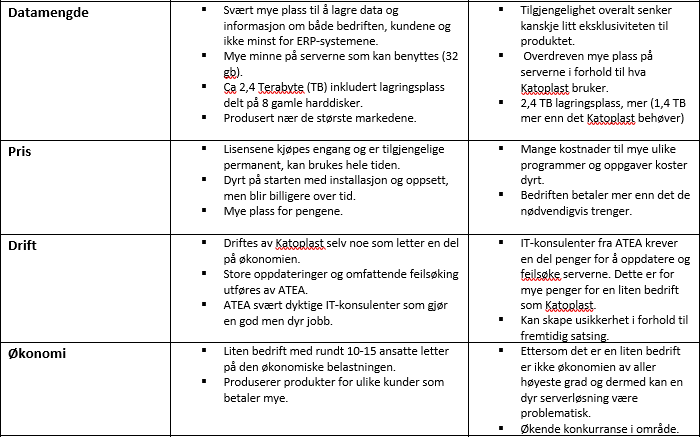
\includegraphics[width=\textwidth]{Bilder/s2.PNG}
%\paragraph{}
%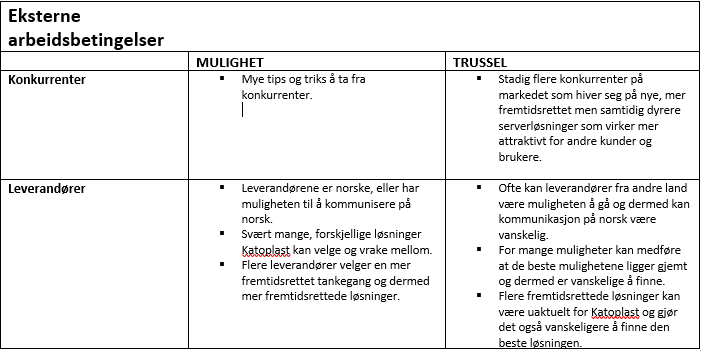
\includegraphics[width=\textwidth]{Bilder/s4.PNG}

% h(ere)t(op) bestemmer hvordan tabellen legger seg (!) betyr den skal forsøke å "force" det.
\begin{longtable}[!ht]{lp{0.4\textwidth}p{0.3\textwidth}} \toprule
	\multicolumn{3}{l}{{\large \textbf{Interne arbeidsbetingelser}}} \\ \midrule
    & \multicolumn{1}{c}{\textbf{Sterke sider}} & \multicolumn{1}{c}{\textbf{Svake sider}} \\ \midrule
    
    \textbf{Server} 
    & % col2 Dette er andre kolonne hvor det står om sterke sider:
    {\scriptsize 
    	\pbox{0.4\textwidth}{%
    	{\tiny \ding{228}} Windows operativsystem for servere. \\ 
    	{\tiny \ding{228}} Backup-software med 3 års oppgradering, 6 backup-taper og 1 rensetape- \\
        {\tiny \ding{228}} Tilpasset ERP-systemene Mamut og Access. \\ 
    	{\tiny \ding{228}} Nok plass til å holde systemene i tillegg til annen data og informasjon. \\
    	{\tiny \ding{228}} Driftet og levert av norske leverandører gjør kommunikasjonen enklere.}} 
    & % col3 Dette er tredje kolonne hvor det står om svake sider:
    {\scriptsize 
    	\pbox{0.3\textwidth}{%
    	{\tiny \ding{228}} Overpriset installasjon og oppsett av server. \\
    	{\tiny \ding{228}} Svært dyre lisenser for programmer som ikke er benyttet. \\
        {\tiny \ding{228}} Svært gammel og utdatert maskinvare som holder serveren i gang. \\
        {\tiny \ding{228}} Benytter seg av svært treg prosessor og gamle harddisker. \\
        {\tiny \ding{228}} Ingen SSD som holder på data.}
    } \\ \cmidrule(l{-0.6in}r){2-3}
    
    \textbf{Sikkerhet} % Nytt tema 
    & % col2 Slik fortsetter det nedover:
    {\scriptsize % setter størrelsen på skriften i denne cellen.
    	\pbox{0.3\textwidth}{% gjør det mulig å bruke linjeskift: \\ inni celler
    	{\tiny \ding{228}} Serverne ligger på huset og er dermed under Katoplasts tilsyn. Dette gir Katoplast følelsen av letterlse ettersom de har oversikt over hvor serverne befinner seg.\\
    	{\tiny \ding{228}} Katoplast er en mindre kjent bedrift og med at serverne ligger på huset minker dette sjangsen for å bli utsatt for et hacker-angrep.
        }
    }
    & % col3 
    {\scriptsize 
    	\pbox{0.3\textwidth}{%
    	{\tiny \ding{228}} Katoplast er ikke verdens sikreste sted og dermed kan tyverier medføre kritiske skader på serverne dersom noen skulle bryte seg inn. \\
    	{\tiny \ding{228}} Serverne er gamle og utdaterte og dette gjør at de kan ha høyere risiko for å feile og dermed skape problemer for Katoplast. 
        }
    } \\ \cmidrule(l{-0.6in}r){2-3}
    
    \textbf{Datamengde}     
    & % col2
    {\scriptsize 
    	\pbox{0.3\textwidth}{%
    	{\tiny \ding{228}} 	Betydelig mer plass til å lagre data og informasjon om både bedriften, kundene og ikke minst for ERP-systemene. \\
    	{\tiny \ding{228}}  Mye minne på serverne som kan benyttes (32 gb).\\
        {\tiny \ding{228}}  	Ca 2,4 Terabyte (TB) inkludert lagringsplass delt på 8 gamle harddisker. \\
        {\tiny \ding{228}} 	Produsert nær de største markedene.  \\
        }
    }
    & % col3 
    {\scriptsize 
    	\pbox{0.3\textwidth}{%
    	{\tiny \ding{228}}	Tilgjengelighet overalt senker eksklusiviteten til produktet.   \\
    	{\tiny \ding{228}} Overdreven mye plass på serverne i forhold til hva Katoplast bruker. \\
        {\tiny \ding{228}} 	2,4 TB lagringsplass, mer (1,4 TB mer enn det Katoplast behøver)  \\
        }
    } \\ \cmidrule(l{-0.6in}r){2-3}
    
    \textbf{Pris}     
    & % col2
    {\scriptsize 
    	\pbox{0.3\textwidth}{%
    	{\tiny \ding{228}}	Lisensene kjøpes engang og er tilgjengelige permanent, kan brukes hele tiden.  \\
    	{\tiny \ding{228}}  	Dyrt på starten med installasjon og oppsett, men blir billigere over tid.\\
        {\tiny \ding{228}} 	Mye plass for pengene. \\
        }
    }
    & % col3 
    {\scriptsize 
    	\pbox{0.3\textwidth}{%
    	{\tiny \ding{228}}  	Mange kostnader til flere ulike programmer og oppgaver koster dyrt. \\
    	{\tiny \ding{228}}	Bedriften betaler mer enn det de nødvendigvis trenger.   \\
        }
    } \\ \cmidrule(l{-0.6in}r){2-3}
    \textbf{Drift}     
    & % col2
    {\scriptsize 
    	\pbox{0.3\textwidth}{%
    	{\tiny \ding{228}} 	Driftes av Katoplast selv noe som letter på økonomien. \\
    	{\tiny \ding{228}} 	Store oppdateringer og omfattende feilsøking utføres av ATEA.  \\
        {\tiny \ding{228}} 	ATEA svært dyktige IT-konsulenter som gjør en god men dyr jobb.  \\
        }
    }
    & % col3 
    {\scriptsize 
    	\pbox{0.3\textwidth}{%
    	{\tiny \ding{228}} 	IT-konsulenter fra ATEA krever store summer for å oppdatere og feilsøke serverne. Dette er for store summer for en liten bedrift som Katoplast.  \\
    	{\tiny \ding{228}} 	Kan skape usikkerhet i forhold til fremtidig satsing.  \\
        }
    } \\ \cmidrule(l{-0.6in}r){2-3}
    \textbf{Økonomi}     
    & % col2
    {\scriptsize 
    	\pbox{0.3\textwidth}{%
    	{\tiny \ding{228}} 	Liten bedrift med rundt 10-15 ansatte letter på den økonomiske belastningen. \\
    	{\tiny \ding{228}} 	Produserer produkter for ulike kunder som betaler mye.  \\ 
        }
    }
    & % col3 
    {\scriptsize 
    	\pbox{0.3\textwidth}{%
    	{\tiny \ding{228}} 	Ettersom det er en liten bedrift er ikke økonomien av aller høyeste grad og dermed kan en dyr serverløsning bli problematisk. \\
    	{\tiny \ding{228}} 	Økende konkurranse i område \\
        }
    } \\ \addlinespace[2mm]\midrule[\heavyrulewidth]\addlinespace[1mm]
    \multicolumn{3}{l}{{\large \textbf{Externe arbeidsbetingelser}}} \\ \midrule
    & \multicolumn{1}{c}{\textbf{Mulighet}} & \multicolumn{1}{c}{\textbf{Trussel}} \\ \midrule
    \textbf{Konkurrenter}     
    & % col2 Til vi kommer hit, hvor nMulighet begynner:
    {\scriptsize 
    	\pbox{0.3\textwidth}{%
    	{\tiny \ding{228}}	Tips og triks å ta fra konkurrenter.   \\
        }
    }
    & % col3 Og her er Trussel:
    {\scriptsize 
    	\pbox{0.3\textwidth}{%
    	{\tiny \ding{228}} 	Stadig flere konkurrenter på markedet som hiver seg på nye, mer fremtidsrettet men samtidig dyrere serverløsninger som virker mer attraktivt for andre kunder og brukere.    \\
        }
    } \\ \cmidrule(l{-0.6in}r){2-3}
    \textbf{Leverandører}     
    & % col2
    {\scriptsize 
    	\pbox{0.3\textwidth}{%
    	{\tiny \ding{228}} 	Leverandørene er norske, eller har muligheten til å kommunisere på norsk. \\
    	{\tiny \ding{228}} 	Svært mange, forskjellige løsninger Katoplast kan velge og vrake mellom.  \\
        {\tiny \ding{228}} 	Flere leverandører velger en mer fremtidsrettet tankegang og dermed mer fremtidsrettede løsninger. \\
        }
    }
    & % col3 
    {\scriptsize 
    	\pbox{0.3\textwidth}{%
    	{\tiny \ding{228}} 	Ofte kan leverandører fra andre land være muligheten å gå og dermed kan kommunikasjon på norsk bli innviklet.   \\
    	{\tiny \ding{228}} 	For mange muligheter kan medføre at de beste mulighetene ligger gjemt og dermed er kompliserte å finne.  \\
        {\tiny \ding{228}}	Flere fremtidsrettede løsninger er uaktuelt for Katoplast og gjør det også vanskeligere å finne den beste løsningen.   \\
        }
    } \\ \cmidrule(l{-0.6in}r){2-3}
\end{longtable}

\section{Spørreundersøkelse}
\paragraph{}For å kartlegge Katoplast sin situasjon i dag, og samtidig også få en oversikt over hvordan Katoplast ønsker at det skal gå for løsningene i fremtiden valgte gruppen å lage en spørreundersøkelse for å kartlegge nettopp dette. Med spørreundersøkelsen ønsket gruppen å finne ut av hvordan daglig lederen rangerer bedriften sin situasjon i dag, og hva slags funksjoner og komponenter ved en server de ønsker skal være med.

\paragraph{} Med hensyn til Katoplast sine kravspesifikasjoner og deres ønsker utarbeidet gruppen en spørreundersøkelse som skulle svare på det gruppen lurte på, og samtidig det gruppen trengte for å kunne gå videre med å finne en passende løsning.

\paragraph{}Undersøkelsen tok for seg en rekke arbeidskrav hvor Katoplast rangerte hvert arbeidskrav på en skala fra 1-10. Gjennom den tilbakemeldingen som ble gitt, valgte gruppen å lage en arbeidskravsanalyse som skulle ta for seg de ulike kravene som bedriften har stilt for prosjektet. Analysen vil gå grundig gjennom de ulikene kravene som er fastsatt for å støtte gruppen i arbeidet med de ulike analysene av løsningene og ikke minst hjelpe gruppen med å finne den riktige løsningen som vil passe for Katoplast. Resultatene på spørreundersøkelsen er som vist på figur 4.1. 

\paragraph{} En arbeidskravsanalyse tar for seg de grunnleggende elementene som er mest fundamental for å løse bedriftens server problem. For å finne best mulig løsningene må arbeidskravene bli sammenlignet opp mot de forskjellige serverløsningene som er mest relevante for en riktig serverløsning.

\paragraph{}I denne analysen er det plukket ut de viktigste elementene for hvordan Katoplast kan finne en serverløsning som passer de best. De blå kolonnene forteller hvor katoplast ligger i dag, og de oransje forteller hva slags krav katoplast ønsker at deres nye server skal legge vekt på.

\begin{figure}[h] % liten h, ikke stor H  ---Ole
\centering
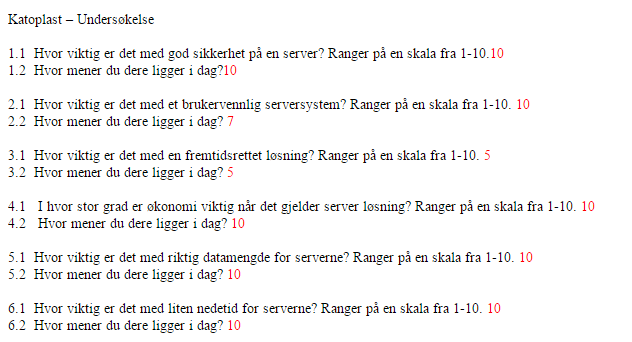
\includegraphics[width=6.5in]{Bilder/sporre.png}
\caption{Spørreundersøkelse}
\end{figure}

\section{Skytjenester}
\subsection{Forbehold} 
\paragraph{} Under blir en rekke sky løsninger presentert som er aktuelle for bedriften Katoplast og som kan eventuelt løse server problemet til Katoplast dersom de skulle ønske å gå for en av disse løsningene. Gruppen er klar over at bedriften ikke ønsker seg en skyløsning, men samtidig forsøker prosjektgruppen å gi Katoplast et nytt syn på skytjenester gjennom de resultatene og den forskningen som har blitt gjort.
\subsection{Technet}
180 000 IT-brukere i 23 land og 6 verdensdeler får skytjenester levert fra Technet sitt datasenter. De 4 største grunnene til å velge komplett skytjenester fra Technet er: 
\begin{enumerate}[noitemsep]
\item Bedriften velger selv applikasjonene de ønsker å bruke, bedriften kan benytte sine fagapplikasjoner i Technet sin skytjeneste. 
\footnote{http://www.xn--skylsninger-jgb.no/skytjenester/}

\item Bedriften kan jobbe hvor som helst. Det vil si alt som behøves er internettforbindelse og en nettleser. Da kan man jobbe fra hele verden.

\item Det kan jobbes på ulike enheter. Det vil si uansett hvilken enhet bedriften bruker, om det er nettbrett, telefon eller datamaskin så vil man ha full tilgang til alle applikasjoner og filer.

\item Hele ansvaret ligger hos Technet. De tar for seg ansvaret for sikkerheten, oppdateringer og at alt fungerer som det skal. 
\end{enumerate}

\paragraph{} Ulike bedrifter har ulike behov. Technet hjelper til med å effektivisere IT-driften i sine skytjenester ut fra bedriftens situasjon i dag og dens fremtidige målsetninger. Technet tilbyr ulike nivåer av skytjenester. Alt fra driftsstøtte og hosting, til sentralisert IT-drift og håndtering av komplette IT-systemer leveres i Technet sin skytjeneste.

\paragraph{} Katoplast kan benytte alle sine fagapplikasjoner i Technet sine skytjenester. Super Office, Visma, Autocad, Mamut, Handyman, Evatic, Solidworks, DI systemer, Maestro, Sticos, PAT, Adobe og Extensor er eksempler på løsninger Technet sine kunder benytter i skytjenesten i dag. \footnote{http://www.technet.no/skytjenester/skytjenester/hvorfor-skytjenester.aspx}

\paragraph{}Lokal IT-drift stiller krav til fysisk nærvær av intern eller ekstern kompetanse. Hvordan håndteres oppgraderinger, virusangrep, backup eller ekstraordinære hendelser etter arbeidstid? Technet kan gjennom skytjenesten tilby profesjonell support døgnet rundt og brukerstøtte direkte på skjermen. I dag er ofte sikkerheten delegert ned til hver datamaskin, som igjen medfører at den største sikkerhetsrisikoen ligger hos den enkelte medarbeider. En skytjeneste gjør det enklere å holde riktig sikkerhetsnivå mot uønsket innlogging, datavirus, sikkert samband, automatisk backup og mot risikoen for å miste data ved brann eller tyveri.

\subsection{Microsoft Azure}
\begin{figure}[H]
\centering

\includegraphics[width=4.2in]{Bilder/azure.png}
\caption{Logoen til Microsoft Azure (Msazurelogo,2015)}
\end{figure}

\paragraph{} Microsoft Azure er en nettsky-basert databehandlings tjeneste lagd av Microsoft. Azure er til for å bygge, utplassere og administrere applikasjoner og tjenester igjennom et globalt nettverk av microsofts egne data-senter. Azure tilbyr blant annet PaaS, IaaS og SaaS tjenester for sine kunder. 
\footnote{https://azure.microsoft.com/nb-no/overview/what-is-iaas/}
\footnote{http://robertgreiner.com/2014/03/windows-azure-iaas-paas-saas-overview/}

\paragraph{} Microsoft sin skyløsning tilbyr en helt egen måte å gjenopprette data på kalt "Site Recovery". Azure tillater brukerne å danne egne gjenopprettingsplaner. Dette er planer som tillater brukerne å planlegge for nødssituasjoner og ikke minst forebygge problemer med data og informasjon. I tillegg tilbyr Azure også automatisk beskyttelse av de virtuelle maskinene som bedriften benytter. Tjenesten er laget for å kunne gjenopprette selv de mest komplekse systemene innenfor en bedrift.
\footnote{https://azure.microsoft.com/nb-no/services/site-recovery/}

\subsection{Amazon Web Services}
\begin{figure}[H]
\centering

\includegraphics[width=4.2in]{Bilder/AWS.png}
\caption{Logoen til Amazon Web Services (Amazon Web Services, 2016)}
\end{figure}
\paragraph{}Amazon Web Services eller AWS er datterselskapet til den kjente Amazon.com. AWS tilbyr en on-demand platform for skytjenester. Fra og med 2016 tilbyr AWS mer enn 70 forskjellige tjenester. Dette inkluderer altså lagring, databaser, analysering, applikasjonstjenester, utplassering, ledelse, utviklerverktøy og networking. Disse tjeneste operer fra 16 forskjellige regioner spredt rundt i verden.
\footnote{ https://aws.amazon.com/application-hosting/benefits/ }
\footnote{ https://npifinancial.com/blog/pros-and-cons-digging-into-amazon-web-services/ }
\footnote{ https://npifinancial.com/blog/pros-and-cons-digging-into-amazon-web-services/ }

\paragraph{}Amazon Elastic Compute Cloud, bedre kjent som Amazon EC2 gir brukerne muligheten til å leie virtuelle datamaskiner hvor brukeren kan kjøre deres egne applikasjoner. EC2 oppmuntrer skalerbar utplassering, dette vil altså si at brukeren kan bruke Amazon sine web-tjenester til å starte et Amazon Machine Image ("AMI") til å konfigurere en virtuell maskin, som inneholder alt ønskelig software. Ved bruk av EC2 betaler du kun for timene du bruker, derav "Elastic". EC2 tilbyr også brukerne tilgang til de 16 forskjellige regionene, dette igjen tillater optimalisering av ventetid ("latency") og et høyt nivå overflødighet.
\footnote{http://docs.aws.amazon.com/AWSEC2/latest/UserGuide/concepts.html}
\footnote{https://aws.amazon.com/ec2/}


\paragraph{}Amazon Simple Storage Service, eller S3 gir brukeren mulighet til å lagre data igjennom web-tjenester. I følge til Amazon er målet med S3 sitt design å skaffe skalering, høy tilgjengelighet og lav ventetid.
\footnote{ https://aws.amazon.com/s3/pricing/ }
\footnote{ https://aws.amazon.com/s3/ }
\footnote{http://docs.aws.amazon.com/AWSEC2/latest/UserGuide/concepts.html}
\paragraph{}Amazon AWS lanserte i 2006, og nå 11 år senere er det i god stand, og høyt rangert som en ren nettsky-basert løsning.


\section{PC Hjelp AS - Intern løsning}
\paragraph{}PC Hjelp AS har gitt gruppen et tilbud. Når man benytter seg av interne servere på huset vil man kunne ha full kontroll over sine egne servere. Man trenger ikke å forholde seg til noen andre, man drifter det meste selv, eller gjennom et IT-team. Serverne blir bygget etter selskapets behov og vil kunne oppgraderes hvis det skulle vært ønsket.
\footnote{http://www.dwuser.com/education/content/why-you-need-a-testing-server-and-how-to-do-it/}



\paragraph{} Når man leter etter en serverløsning som er intern er man avhengig av hardware, software og konsulentarbeid. De forskjellige løsningene prosjektet vil fremstille for Katoplast vil være avhengig av det Katoplast trenger.  Det er essensielt at de løsningene som presenteres ikke har noen svakheter innen hardware eller software opp imot behovet til katoplast. Når det kommer til konsulentjobben kommer den til å bli betalt ut fra timene de trenger for å gjøre jobben gjort, altså ikke for spesifikke egenskaper som er mer relevant for software og hardware. Vesentlig for vurderingen av tilbudet er å vurdere erfaringene til konsulentene i fagfeltet. 
\footnote{http://www.dwuser.com/education/content/why-you-need-a-testing-server-and-how-to-do-it/}
\footnote{http://whatismyipaddress.com/localhost}
\footnote{http://www.episerver.com/learn/resources/blog/udaiappa-ramachandran/the-pros-and-cons-of-cloud-storage/}

\paragraph{} PC Hjelp AS ga prosjektet et tilbud på software, hardware og konsulentarbeidet rundt servere. Disse er tilpasset behovene til Katoplast.
\subsection{Tilbudsinformasjon}
\begin{description}
\item Hardware: Lenovo ThinkServer, 1 x Xeon E3-1225v5, 1x16GB 2x 1TB 3,5* SATA Slim DVD-RW 250W. Pris: 10072,00 kr.
\item Software: Microsoft Windows Server 2012. 
\item Pris: 7192,00 kr
\item Konsulentarbeid: Timespris konsulent Lars Berge. 
\item Pris: 790,00 kr pr. time
\end{description}
  
 
\section{Hybrid Cloud Løsninger}
\subsection{Forbehold}
\paragraph{} Løsningene under tilhører kategorien Hybride Cloud Løsninger. Dette er løsninger som tar for seg den komplekse strukturen og arkitekturen til en hybrid cloud hvor lagringsystemet deles i 2, en public og en private cloud (Figur 4.3). En slik løsning vil Katoplast oppleve en økning i muligheter for lagring og deling av informasjon og ikke minst oppleve en ny form for sikkerhet når det gjelder backup av filer og annen data. I tillegg vil de fleste leverandørene av en Hybrid Cloud være åpne til å gi full støtte til Katoplast med deres installasjon og oppsett av en slik, fremtidsrettet serverløsning. 

\addcontentsline{toc}{section}{Hybrid Cloud Figur}
\section*{}
\begin{figure}[H]
\centering

\includegraphics[width=6.5in]{Bilder/Hybrid-cloud.jpg}
\caption{Forenklet figur av en Hybrid Cloud. (Roadmap, 2016)}
\end{figure}

\paragraph{} Hver av disse løsningene har sine fordeler og ulemper som gjør dem både unike og samtidig skiller dem fra hverandre. Deres priser er svært varierende og gruppen har tatt i betraktning de spesifikasjonene og ønskene Katoplast har satt for prosjektet i jakten på å finne den beste løsningen. Flere av løsningene som ble diskutert i gruppen ble utelukket etter en grundig vurdering av pris, tilgjengelighet og sikkerhet. Blant annet ekskluderte gruppen Amazon Web Services (AWS) fra dette prosjektet som følge av de alt for høye kostnadene når det gjelder kjøp og installasjon av en hybrid cloud.

\subsection{Microsoft Azure StorSimple}
\paragraph{} Et av verdens største organisasjon innenfor IT har tatt et stort steg innenfor en fremtidsrettet løsning for bedrifter når det gjelder lagring av informasjon og data. Microsoft sin forskning og dyktige arbeidere har utviklet sin egen løsning for en Hybrid cloud for å skape noe unikt, men samtidig også skape noe som kan benyttes av både store og små bedrifter og ikke minst privatpersoner. Microsoft tilbyr flere, forskjellige former av en Hybrid Cloud og er villige til å tilpasse nettskyen for bedriften akkurat slik de ønsker å ha det. Med deres forskjellige tilbud kan dette bli noe som vil være av interesse for Katoplast. Microsoft Azure StorSimple er den nye formen for hybrid sky som tilbyr bedrifter en helt ny form for lagring av data.
\footnote{https://azure.microsoft.com/nb-no/services/storsimple/}

\addcontentsline{toc}{section}{Microsoft StorSimple}
\section*{}
\begin{figure}[H]
\centering
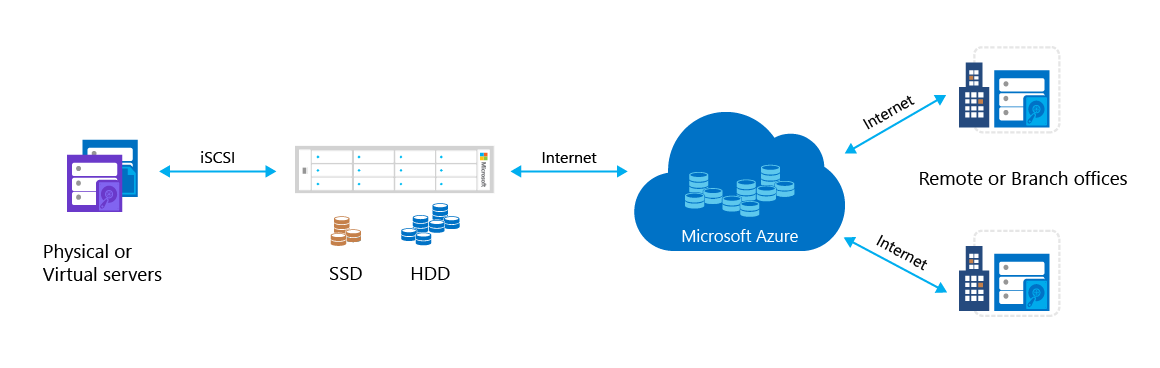
\includegraphics[width=6.5in]{Bilder/storsimple.png}
\caption{StorSimple infrastruktur (StorSimple, 2017)}
\end{figure}

\paragraph{} Med betraktning på Katoplast sine svar på undersøkelsen, har gruppen undersøkt nøye hvilke fordeler som følger med StorSimple. Et av Katoplast sine ønsker var å minke eller automatisere de manuelle, administrative oppgavene som måtte gjennomføres. StorSimple tilbyr nettopp dette med deres automatiserte dataadministrasjon. Med en slik fordel vil Katoplast nå slippe å vedlikeholde store deler av en server, men derimot ha muligheten til å fokusere på andre oppgaver. StorSimple vil arkivere unødvendig data helt automatisk samtidig som den tar seg av vedlikehold av infrastrukturen. Det vil si at de administrative oppgavene som Katoplast arbeider med, blir gjort av StorSimple automatisk. 
\footnote{http://cdn2.hubspot.net/hub/65157/file-1187005090-pdf/StorSimple\_SolutionOverview07-9-14}
\footnote{https://azure.microsoft.com/nb-no/services/storsimple/}

\paragraph{} Et annet konsept med Microsoft sin hybride sky StorSimple er at den legger et stort fokus på backup lagring og nød gjenoppretting av filer og data. Dette er en vesentlig funksjon dersom Katoplast sine servere skulle møte på motgang, nedetid eller at data eventuelt skulle bli slettet eller bli korrupt av ulike årsaker. StorSimple gjør gjenopprettingen av data brukervennlig, og ikke minst tillater den å gjenopprette store datamengder slik at ingenting går tapt. Dermed vil det ikke være noe problem dersom serverne skulle miste informasjon ettersom bedriften vil ha mulighet til å hente tilbake disse. Når det gjelder gjenoppretting av data er dette ofte en smertefull og stressende prosess som må gjøres manuelt på interne servere. StorSimple vil ta seg av alt dette arbeidet og gjøre det så simpelt som mulig for brukerne av nettskyen.
\footnote{https://docs.microsoft.com/en-us/azure/storsimple/storsimple-manage-backup-policies}
\footnote{https://azure.microsoft.com/nb-no/solutions/hybrid-integration/}

\paragraph{} StorSimple er naturligvis et relativt nytt konsept som fortsatt er i utvikling og som vil få mange flere funksjoner i nær fremtid. videre, er det slik at prisene på StorSimple sine tjenester er svært varierende. Tjenesten tilbyr brukere å velge hvor stor lagringsplass de ønsker å kjøpe, om diskene skal være SSD eller HDD og samtidig tilbyr tjenesten ulike abonnement for å tilpasse tjenesten til flere. Basert på den informasjonen som gruppen har samlet fra Katoplast og deres ønsker, har prosjektgruppen funnet en løsning som kan være rimelig, men samtidig kostbar for Katoplast.
\footnote{https://azure.microsoft.com/en-us/pricing/}

\paragraph{} StorSimple deles inn i 2 deler, en fysisk og en virtuell del. Her vil bedrifter og brukere ha muligheten til å velge ulike servere og hvor mange av hver server de ønsker å kjøpe. Hver server har sine, unike fordeler. Modellene på serverne varierer og Microsoft introduserer hele tiden nye modeller. For nå tilbyr Microsoft 2 fysiske apparater, modell 8100 og modell 8600, og 3 virtuelle apparater, modell 8010, modell 8020 og modell 1200. 
\footnote{https://docs.microsoft.com/en-us/azure/storsimple/storsimple-technical-specifications-and-compliance}

\paragraph{} Microsoft tilbyr deres kunder flere måter å kjøpe deres sky tjenester på. Hver av disse metodene er tilpasset ulike kunder og er skapt for å gjøre deres skytjenester tilgjengelig for flere bedrifter og brukere. Et av alternativene siktet mot større bedrifter er en metode kalt "foretaksavtaler". Med en foretaksavtale vil store organisasjoner inngå en avtale med Microsoft om forskuddsbetaling av tjenestene de får.
\footnote{https://azure.microsoft.com/nb-no/pricing/purchase-options/}
\footnote{https://azure.microsoft.com/nb-no/pricing/enterprise-agreement/}

\paragraph{} En annen måte å kjøpe tjenestene på er gjennom Microsoft sitt eget "open-licensing program". Dette er en kjøps metode ment for små til middels-store bedrifter som ønsker å benytte seg av Microsoft sine sky tjenester. Dette er en metode som er simplifisert for bedrifter og som gir større kontroll og oversikt over investeringen. Samtidig tilbyr denne kjøpsmetoden også mindre bedrifter å få deres pris redusert over flere år.
\footnote{https://www.microsoft.com/en-us/licensing/licensing-programs/open-license.aspx}

\paragraph{} En tredje metode for kjøp av nettskyene til Microsoft er gjennom Microsoft partnere. Bedrifter vil ha muligheten til å kjøpe en Microsoft partner som hjelper bedriften med å implementere og opprettholde den beste løsningen for en nettsky. Disse er også kunnskapsrike konsulenter som kan hjelpe med kostnader og andre spørsmål som en bedrift har.
\footnote{https://azure.microsoft.com/nb-no/partners/directory/}

\paragraph{} Microsoft introduserer ofte nye konsepter som de ønsker å virkeliggjøre, og et av deres nye ideer, Nano Server, er fundamentalt for deres cloud og hybride løsninger som de tilbyr brukerne sine.
\footnote{https://www.pluralsight.com/blog/it-ops/microsoft-nano-server-announced}

\subsection{VMware vCloud Air}

\paragraph{} En annen rimelig Hybrid løsning for Katoplast er VMware vCloud Air Hybrid. Dette er VMware sitt svar på en hybrid nettsky hvor datalagring foregår både i skyen og lokalt.VMware gjør det lett for brukere av deres nettsky hvor de samme programvarene benyttes for å gjennomføre lagring og andre type prosesser for både den interne og eksterne nettskyen. I tillegg til dette tillater VMware at prosesser gjennomføres fortløpende uten nedetid, hvor bedriften vil ha mulighet til å legge inn alt av data og informasjon samtidig som de arbeider. Leverandøren tillater også brukere av nettskyen å planlegge tidspunkt hvor de ønsker å legge inn data eller manipulere data. Dette er en nyttig funksjon å ha dersom man ønsker å spare unødvendig arbeid når det gjelder å komme i gang med nettskyen, men at man heller planlegger når man ønsker å gjennomføre endringene. Slik vil nettskyen være forberedt på at det skjer endringer og dermed også unngå problemer.
\footnote{http://www.vmware.com/solutions/cloud-computing.html}
\footnote{http://www.vmware.com/products/cloud-foundation.html}

\addcontentsline{toc}{section}{VMware Hybrid Cloud}
\section*{}
\begin{figure}[H]
\centering
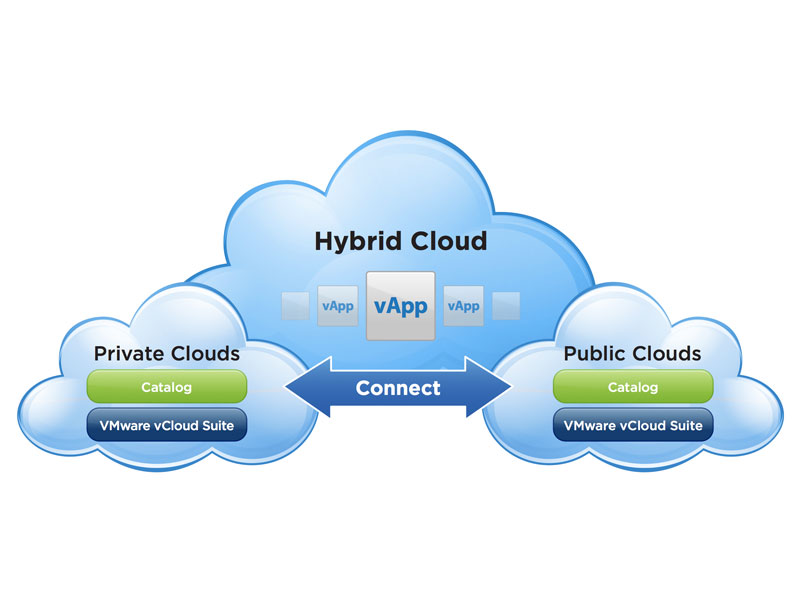
\includegraphics[width=5.5in]{Bilder/vmware.jpg}
\caption{VMware sin Hybride Sky Infrastruktur. Viser hvordan vCloud Suite er koblet opp mot skyene og hvordan disse er koblet sammen. (VMware, 2014)}
\end{figure}


\paragraph{} Videre, så følger VMware et simpelt og brukervennlig tankesett. De ønsker at deres tjenester skal kunne benyttes av så mange som mulig og samtidig være så enkle som mulig. Med tanke på dette har VMware utviklet egne funksjoner, verktøy og innebygde prosesser som deres kunder kan benytte seg av og som tar for seg de administrative oppgavene og andre tunge oppgaver. En fordel med dette er at VMware også støtter flere operativsystemer noe som er avgjørende for Katoplast som kjenner best til Windows Operativ System (OS). 
\footnote{http://www.vmware.com/products/vrealize-suite.html}

\paragraph{} I tillegg har VMware lagt et stort fokus på brukervennlighet når det gjelder deres sky tjenester. Som følge av dette introduserer VMware "vCloud Suite" som er en platform for administrasjon og kontroll av deres sky tjenester. Med vCloud Suite vil mange av de administrative oppgavene gjøres helt automatisk. Tjenesten gjør det også lett for bedrifter å oppgradere eller nedgradere deres hybride løsning bare ved noen få tastetrykk.
\footnote{http://www.vmware.com/products/vrealize-automation.html}
\footnote{http://www.vmware.com/products/vcloud-suite.html}

\paragraph{} Som Microsoft, tilbyr også VMware ulike kjøps metoder når det kommer til deres skyløsninger. I likhet med Microsoft deles også disse i 3 og hver av disse med deres egne fordeler og ulemper, basert på hva bedriften ønsker.
\footnote{https://vcloud.vmware.com/uk/service-offering/pricing-calculator}

\paragraph{} Et av kjøps alternativene som VMware tilbyr kalles "OnDemand" og tilbyr brukere å kun betale for den lagringsplassen de benytter seg av uten å skrive en kontrakt eller noen form for abonnement. For eksempel, dersom Katoplast skulle bruke opp 500gigabyte (gb) lagringsplass ut av 1 terabyte, vil Katoplast kun behøve å betale for de 500 gb de bruker og ikke for de hele 1 TB. Dette alternativet passer best for mindre bedrifter som ikke bruker stort mye plass og dermed kan spare penger på dette.
\footnote{https://vcloud.vmware.com/uk/service-offering/pricing-calculator/on-demand}

\paragraph{} Den andre metoden baserer seg på abonnement. Bedrifter har muligheten til å velge fra ulike abonnement som VMware tilbyr. Fordelen med dette er at man vil ha muligheten til å forutse prisene samt at man vil få tilgang til flere ressurser for å skape en kjappere og bedre server løsning. Et slikt alternativ vil passe for større bedrifter som vet hvor mye lagringsplass de benytter og ønsker tilgangen til flere ressurser for å forbedre deres servere.
\footnote{https://vcloud.vmware.com/uk/service-offering/pricing-calculator/subscription}

\paragraph{} "Horizon Air" er VMware sitt tredje kjøps alternativ og legger vekt på bedrifter som ønsker å benytte seg av virtuelle maskiner og applikasjoner. Velger man Horizon Air vil man inngå et abonnement med VMware hvor man vil ha muligheten til å kjøpe virtuelle maskiner, apper og samtidig ha muligheten til den beste formen av nød gjenoppretting av informasjon og data.
\footnote{http://www.vmware.com/cloud-services/desktop/horizon-cloud-on-premises.html}
\footnote{http://www.vmware.com/cloud-services/desktop/horizon-cloud-hosted.html}

\newpage
\section{Priser}
\paragraph{} Under vil du finne et linjediagram som viser prisene på de ulike bedriftene over flere år. Prisene er sortert på hvert år fra 2017 til utover 2025.
Dette gir bedriften en oversikt over server-budsjettet i fremtiden blant de forskjellige løsningene. 

\addcontentsline{toc}{section}{Microsoft StorSimple}
\section*{}
\begin{figure}[H]
\centering
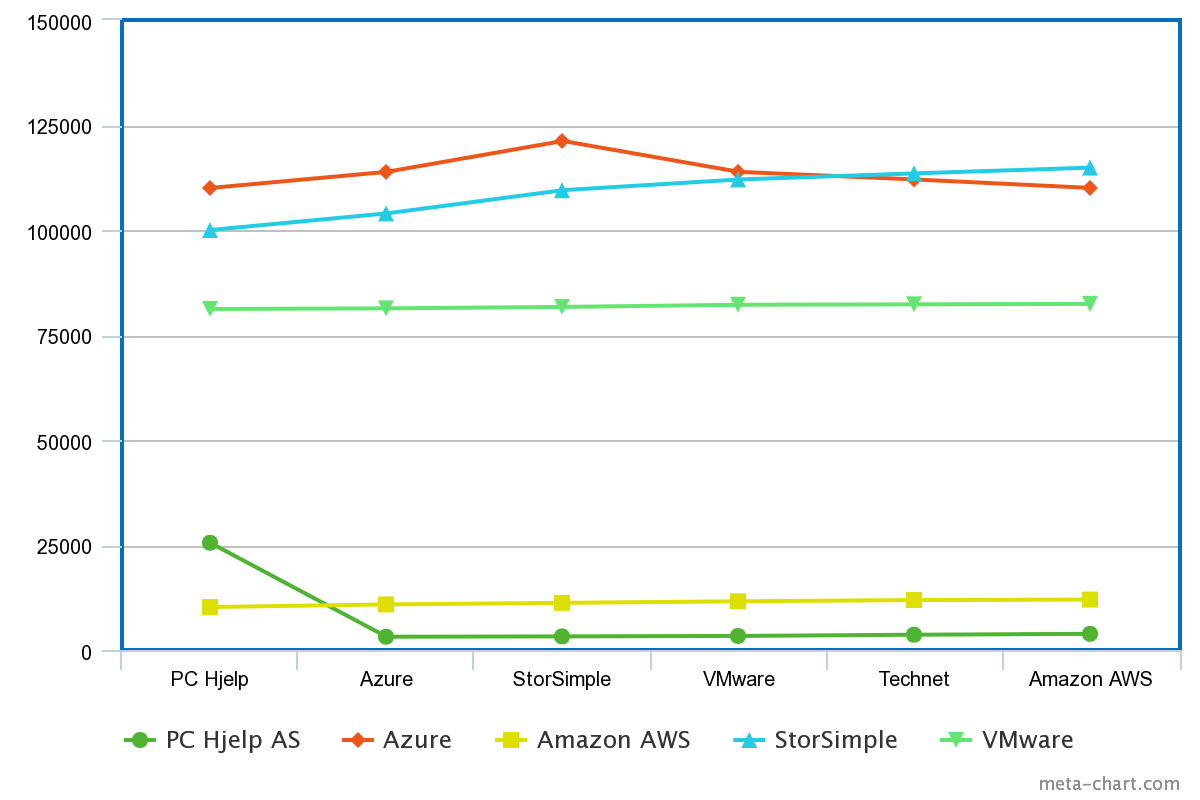
\includegraphics[width=5.5in]{Bilder/priser2.png}
\caption{Serverløsninger Priser}
\end{figure}
\chapter{Diskusjon}

\paragraph{}I dette kapittelet blir de ulike resultatene diskutert frem til en løsning. Dette kapittelet er en grundig undersøkelse, vurdering og forskning av alle løsninger. Her er målet å skape en objektiv diskusjon for å komme frem til en konkret og verdig løsning for problemet til Katoplast. 

\paragraph{}Ut i fra produktalternativene nevnt i punkt 4 ser vi at det finnes en rekke brukbare løsninger som kunne ha passet behovet til Katoplast. I disse produktalternativene finnes løsninger som skytjenester, Interne tjenester og hybrid tjenester. Ut ifra disse måtte prosjektet gjøre en vurdering av hvilke tjenester som skulle passe behovet til Katoplast best. 

\paragraph{} For at prosjektet skulle finne den beste løsningen til Katoplast valgte gruppen å lage en arbeidskravsanalyse opp i mot alle løsningene. I denne arbeidskravsanalysen tok prosjektet de samme arbeidskravene som gruppen hadde med i spørreundersøkelsen (3.1). Der ifra rangerer gruppen hvert av arbeidskravene fra en skala 1-100. Dette gjorde det lettere å kunne sammenligne med spørreundersøkelsen (3.1). Styrken med dette gjorde at gruppen kunne se hvilke løsning som ville treffe best etter behovet til Katoplast. Arbeidskravsanalysene som ble gjennomført ga en pekepinn på hvor prosjektet burde strekke seg.


\paragraph{} Tatt i betrakning er det noen arbeidskrav som veier opp mer enn andre. Når det kommer til sikkerhet, økonomi og nedetid er dette arbeidskrav som blir rangert høyere enn de andre arbeidskravene. Dette er de mest relevante arbeidskravene, og de har dermed størst betydning for prosjektets konklusjon.

\section{PC Hjelp AS}
\paragraph{} Det å finne en intern serverløsning for bedriften Katoplast var ikke den enkleste oppgaven. Leverandører av serverne var ikke åpne for å gi ut sine priser og løsninger. Etter mange samtaler med ulike leverandører over telefon og e-post, var det utfordrende å finne en løsning som var brukbar. PC Hjelp AS, arrangerte et møte med gruppen, hvor de presenterte sin løsning som kan være av interesse for Katoplast. 
\subsection{Fordeler}

\paragraph{} Interne servere kan ha kraftig sikkerhet dersom man er flinke til å oppdatere og vedlikeholde systemet. Tar man jevnlig backup og opprettholder backup-disken et annet sted enn der hvor serveren befinner seg, er det nesten umulig å miste data. Interne servere kan være kompliserte å drifte dersom man gjør dette selv. De fleste bedrifter benytter seg av IT-konsulenter for drift, men dette koster ofte en stor formue for få timers arbeid -derfor velger mange bedrifter heller å gjøre dette selv. Skulle noe av hardware gå i stykker er dette også utgifter som bedriften må betale.
\footnote{http://www.dwuser.com/education/content/why-you-need-a-testing-server-and-how-to-do-it/}


\paragraph{} Tilbudet prosjektet fikk tilsendt av PC Hjelpen AS var et langt mer pålitelig tilbud enn det Katoplast har fått tidligere. Hardware var langt mer skreddersydd og treffer langt bedre på de rammene Katoplast trenger. Den største fordelen med denne løsningen er at den letter på det økonomiske trykket som Katoplast opplever. Med en total pris på kun 25 530 kr blir kostnadene betraktelig mindre.

\paragraph{} I tilbudet som legges frem får Katoplast muligheten til å benytte seg av programvare og maskinvare som de allerede er kjent med. PC Hjelp tilbyr nemlig Windows Server 2012 som system. Med 2 x 1 terabyte harddisker får Katoplast mer enn nok lagringsplass til å lagre de verdifulle dataene de har, og samtidig ha nok plass til annen informasjon. Serveren som blir benyttet er Lenovo ThinkServer Xeon E3-1225v5. Dette er en kraftig maskin med 8 gigabyte RAM. Gruppen og PC Hjelpen AS ser ikke noe gevinst i å finne noe nyere software. Dette går kun utover budsjettet. 
\footnote{http://whatismyipaddress.com/localhost}

\paragraph{} Rundt konsulentarbeidet mener PC Hjelp as at de trenger mellom 4 til 7 timer for å implementere de nye serverene. PC Hjelpen tar 790kr i timen, noe som også er veldig rimelig opp mot vanlig konsulentarbeid. Arbeidet til konsulenten inkluderer klargjøring av ny datamaskin, installasjon av basis programmer og virusbeskyttelse. PC Hjelp AS ønsker også å ta en titt på situasjonen til Katoplast i dag for å kunne kartlegge server tilbudet mer effektivt. Dette er svært positivt med tanke på å finne den beste løsningen for Katoplast.

\paragraph{} 

\subsection{Ulemper}

\paragraph{} Ulempene med denne løsningen er at Katoplast først og fremst kommer til å fortsette å ha de administrative oppgavene som de gjerne ville slippe. De må da fortsette med drift og oppdateringer av serverne selv dersom de ikke ønsker å bruke innleide konsulenter. Et av ønskene til Katoplast var å unngå disse administrative oppgavene, men dette er problematisk å oppnå med en intern server som ikke gjør dette automatisk. \footnote{http://www.episerver.com/learn/resources/blog/udaiappa-ramachandran/the-pros-and-cons-of-cloud-storage/}

\paragraph{} En annen ulempe med løsningen er at den er lite fremtidsrettet. Det å ha servere på huset er en gammeldags metode som begynner å forsvinne. Flere og flere velger å gå for en mer fremtidsrettet løsning som en hybrid sky eller en vanlig sky tjeneste. Det er også slik at interne servere ofte opplever problemer med maskinvaren, noe som kan skape mer nedetid og feil som kan hemme arbeidet til bedriften. 

\section{Verdict}
\begin{figure}[H]
\centering
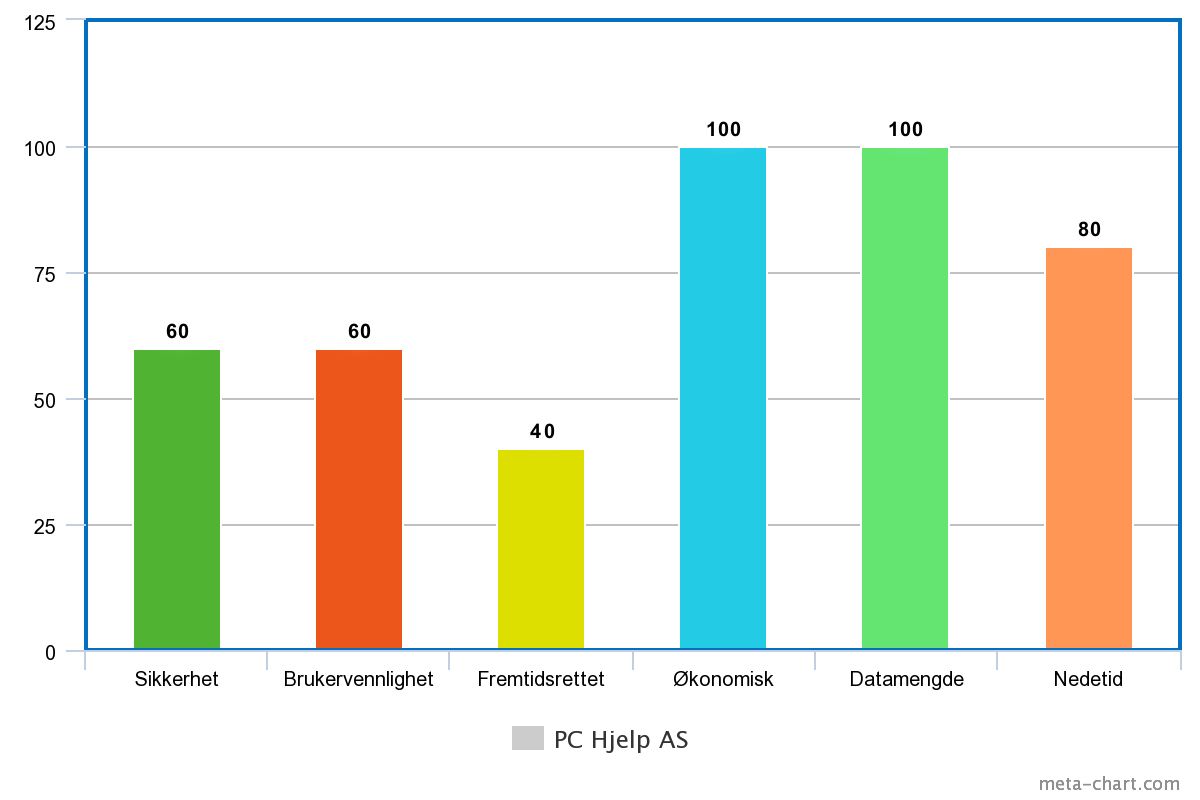
\includegraphics[width=6.5in]{Bilder/pchjelpchart.png}
\caption{Prosjektgruppens rangering av PC Hjelp sin løsning.}
\end{figure}

\section{Sky tjenester}

\subsection{Fordeler med Technet}
\paragraph{}Med sentraliserte IT-systemer i Technet sin skytjeneste, kan ny og krevende programvare settes i drift uten innkjøp av nye PCer og servere, eller behov for lokale oppgraderinger. Alle endringer skjer sentralt i Technet sin skytjeneste og den datakapasiteten som kreves blir produsert i en datasentral og bedriften kan planlegge når endringer skal skje og hvilke rettigheter brukerne skal tildeles i skytjenesten. Bedriften får en garantert oppetid på IT-løsningen, og har tilgang til egen IT-avdeling 24/7/365. Alle endringer skjer sentralt og den datakapasiteten som kreves blir produsert i en datasentral. 
\footnote{http://www.xn--skylsninger-jgb.no/skytjenester/}

\paragraph{} Nøkkelen til en problemfri IT-hverdag og et velfungerende IT-miljø, ligger i samspillet mellom hvert system, hver tjeneste og hver komponent. Brukerens IT-opplevelse avhenger av at alle komponentene, i en lang kjede, fungerer hver for seg og sammen med hverandre. Ved å ta et totalt ansvar kan Technet med sin skytjeneste sikre kvaliteten på komponentene som utgjør helheten. Resultatet er en skytjeneste som gir optimalisert IT-opplevelse for alle brukerne. Skulle et problem i skytjenesten oppstå har Technet ansvaret for alle potensielle feilkilder, enten dette gjelder nettverket, bredbåndslinjer, klienten eller applikasjonen. På den måten sikres i Technet sin skytjeneste effektiv feilsøking- og retting slik at man raskt kommer i gang med arbeidet igjen.


\subsection{Ulemper med Technet}
\paragraph{}Riktig skyløsning for bedriften er like siker som banken. Ulempen er den samme som fordelen- at du alltid er tilgjengelig. Dessuten finnes det så mange varianter av nettbrett og håndholdte enheter at det for en IT-avdeling kan være innviklet å sørge for ugjennomtrengelig sikkerhet. Ettersom bedriften må være avhengig av å måtte være koblet til internett, setter det også en avgrensing på dette. De fleste sky løsningene blir et mål for hackere. Dette setter enda større sikkerhetskrav til brukerne som har tilgang til enhetene. Det er lettere for en hacker å sende en falsk epost til en u-viten bruker på bedriften kontra å hacke technet sine servere. Den ene ulempen gruppen støtet på fra blant annet Technet og andre leverandører var at disse aktørene ønsket direkte kommunikasjon med Katoplast for å gi et pristilbud. Dette var noe som påvirket planleggingsfasen til prosjektgruppen.
\footnote{http://www.xn--skylsninger-jgb.no/om-skytjenester-fra-technet/}


\subsection{Fordeler med Azure}

\paragraph{}Det er mange positive sider med Azure løsningene til Microsoft. Skulle man trenge tilgang til dataene sine kan man lett få tak i disse ved bruk av en smart enhet. Det vil si at man kan ha tilgang på alle dataene sine når som helst, og hvor som helst uten begrensninger. Dette gjør det mulig for ansatte i bedrifter å kunne arbeide hvor som helst, til og med når de sitter hjemme. Man trenger altså ikke å sitte fysisk i lokalene til bedriften får å kunne utføre det arbeidet man er tilgitt. Med en slik fordel vil de ansatte ha muligheten til å arbeide mer effektivt, samtidig som de har mer tid dersom de ikke skulle klare å gjennomføre sine oppgaver på lokalene til bedriften. 
\footnote{https://azure.microsoft.com/nb-no/overview/what-is-azure/}

\paragraph{} En fordel med Azure er at den er brukervennlig. Det er Azure som tar seg av alt konsulentarbeid rundt serveren, og gir en essensiell og sikker måte å ta backup på. Ikke minst gir de muligheten til gjenoppretting med ekstern sikkerhetskopiering. Dette gjør at de sensitive opplysningene til en bedrift vil være helt sikre, selv om de skulle bli slettet eller filer skulle bli korrupte. Man har da muligheten til å gjenopprette slettede filer, eller tilbakestille arbeidet til en tid før det oppsto feil. Dette var en bekymring som Katoplast hadde, og som ønsket en løsning som tilbyr en sikker måte å gjenopprette data på.
\footnote{https://azure.microsoft.com/nb-no/services/site-recovery/}

\subsection{Ulemper med Azure}
\paragraph{} Det finnes i imidlertid en rekke ulemper med Azure. Sky løsninger er ofte et mål for hackere som ønsker å få tilgang til sensitive data og opplysninger. Microsoft som er et av verdens største organisasjoner er svært utsatt for slike angrep. Selv om Microsoft har sikkerhet av aller høyeste nivå, er det utfordrende å forebygge slike hacker angrep, og konsekvensene av angrepene er ofte store. Som følge av dette er det ofte slik at brukere og potensielle kunder holder seg til den gammeldagse metoden av å ha servere på huset. 
\footnote{https://www.scmagazineuk.com/microsoft-update-left-azure-linux-virtual-machines-open-to-hacking/article/575472/}

\paragraph{} En ulempe med Azure er at deres sky tjeneste befinner seg på et eksternt sted i verden som deres kunder ikke vet destinasjonen til. Et av Katoplast sine ønsker var at deres data og informasjon ikke skulle ligge hos en ekstern leverandør, ettersom de ikke ønsker at deres informasjon skal gå på avveie. Dette er en stor ulempe med Azure og med andre sky tjenester generelt, ettersom informasjonen lagres et annet sted en hos bedriften. Som følge av dette opplever Katoplast at deres informasjon ikke er sikker og kan i verste fall bli utnyttet av andre.
\footnote{http://www.biztechmagazine.com/article/2017/01/microsoft-warns-hacked-virtual-machines-are-very-real-threat}

\subsection{Azure Verdict}
\begin{figure}[H]
\centering
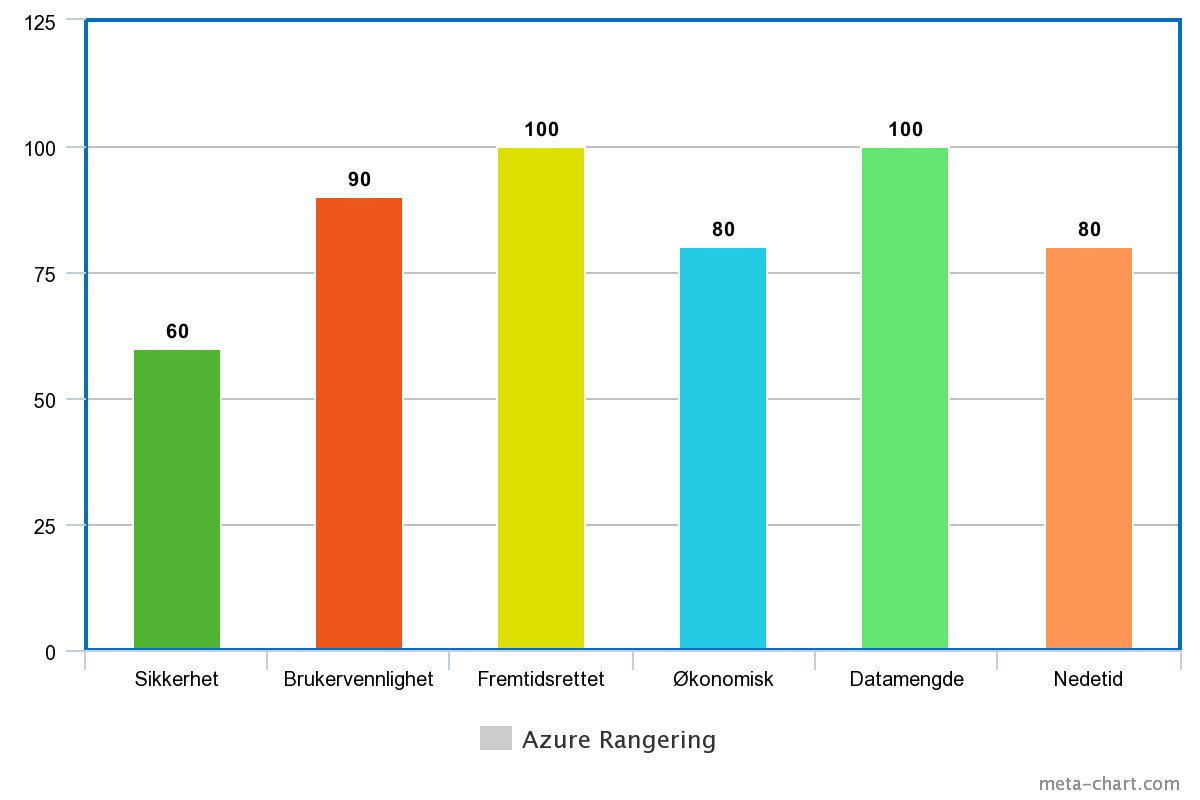
\includegraphics[width=6.5in]{Bilder/azurechart.png}
\caption{Prosjektgruppens rangering av Microsoft Azure.}
\end{figure}

\subsection{Fordeler med Amazon AWS}
\paragraph{} Det kan være en fordel å først og fremst beskrive hva Amazon sitt system tilbyr brukerne. Med Amazon Web Services ønsker Amazon å tilby en skytjeneste som er brukervennlig, fleksibel, kost-effektivt, pålitelig, skalerbar og sist men ikke minst sikker. Fordelen med AWS er at den tilbyr et hav av ulike tjenester og løsninger som brukere kan velge mellom. I tillegg tilbyr de fleksible betalingsmetoder hvor brukerne kun behøver å betale for det de bruker, ikke mer.
\footnote{https://aws.amazon.com/application-hosting/benefits/}

\paragraph{}Amazon AWS har en rekke fordeler. Som en ren skyløsning foregår ingenting internt, her blir det meste tatt hånd om. Derav er AWS veldig brukervennlig. De tilbyr også et bredt spekter av tjenester, som nevnt over, er det 70 forskjellige. De har også spredd rundt på jordkloden, i 16 forskjellige regioner. AWS er også ekstremt nøye på sikkerheten, og påstår at sikkerhet er deres høyeste prioritet. "We worked closely with the Amazon team to develop a security model, which we believe enables us to operate more securely in the public cloud than we can even in our data centers." (Alexander, 2015, AWS re:Invent)
\footnote{https://aws.amazon.com/security/}

\paragraph{} Også verdt å legge merke til, er at alle kontoer registrert i AWS blir lagt inn i en virtuell privat nettsky. Dette bidrar til å styrke sikkerheten rundt deres tjenester og ikke minst bidrar til å forebygge hacking og andre problemer. Det er også gunstig med AWS når selvstendige programvareskapere, slik som Microsoft, selger og inkluderer flere av sine egne produkter i systemet.
\footnote{https://aws.amazon.com/vpc/}

\subsection{Ulemper med Amazon AWS}
\paragraph{} Imidlertid, følger det en rekke ulemper med AWS. Serverene til AWS er alle virtuelle. Selv om klargjøringen er bedre, kan fortsatt ytelsen variere og det virtuelle vil ikke oppleves som like rent og stabilt som fysisk maskinvare. Læringskurven er samtidig bratt for større bedrifter. Dersom man har lite kunnskap innenfor å drifte eller benytte seg av virtuelle systemer, kan dette bli problematisk når man skal overføre arbeidet sitt fra fysiske maskiner til virtuelle systemer. 
\footnote{https://www.togglebox.com/blog/the-cons-of-working-with-amazon-web-services-aws/}
\footnote{https://npifinancial.com/blog/pros-and-cons-digging-into-amazon-web-services/}

\paragraph{} Det er også nødvendig å nevne, at flere små- og mellomstore bedrifter ikke får brukerstøtte og den veiledningen de trenger. Denne type nedprioriteringen er en omfattende ulempe, som kan føre til flere konsekvenser for en bedrift som ikke har den kunnskapen som kreves for drifting og oppsett av servere. Dette gjelder spesielt for Katoplast som, dersom de skulle bytte til en skyløsning, vil oppleve å måtte bruke tid og arbeid i å lære seg dette. Man vil naturligvis ha tilgang til brukerstøtte, men ikke i like stor grad som det andre leverandører tilbyr.
\footnote{https://www.liquidweb.com/blog/why-aws-is-bad-for-small-organizations-and-users/}


\paragraph{} Amazon sine tjenester har også opplevd avbrudd, hvor nedetiden har vart i flere timer. Dette er et problem som Katoplast ønsker å unngå, ettersom deres data og informasjon utgjør alt arbeid som utføres i bedriften. I Katoplast sitt tilfelle kan dette hemme arbeidet og kommunikasjonen innad bedriften og i verste fall føre til tap av penger.
\footnote{http://www.zdnet.com/article/how-amazon-web-services-crashed-and-rose-again/}
\footnote{http://www.geekwire.com/2017/amazon-explains-massive-aws-outage-says-employee-error-took-servers-offline-promises-changes/}

\subsection{Amazon AWS - Pris}
\paragraph{} Som nevnt i fordelene, tilbyr Amazon AWS en veldig fleksibel tjeneste, dette gjelder også prisen. Her betaler du for antall plass du bruker. Dette stiller jo til vesentlig fordel for et selskap som Katoplast som har tilgang til vesentlig mer plass enn de behøver. For kun 500GB arkivert over 40 år. Prisen til AWS avhenger av hvilken region du tilhører, hvis vi som eksempel velger London regionen, ser vi på en pris på rundt 0,0312 dollar pr GB, eller 0,3 NOK. Årlig koster dette cirka 12 000 NOK Som er en passende pris for løsningen. Dette er altså prisen på AWS S3, "simple storage service".
\footnote{https://npifinancial.com/blog/pros-and-cons-digging-into-amazon-web-services/}
\footnote{https://www.datastorageinc.com/blog/amazon-web-services-storage-pros-and-cons-for-document-management}

\section{StorSimple - Hybrid}
\subsection{Fordeler med StorSimple}
\paragraph{} StorSimple deles inn i 2 apparater hvor brukere kjøper et ønsket antall av virtuelle og fysiske apparater. Det finnes flere ulike modeller og hver av disse med deres egne fordeler. For Katoplast virket den beste løsningen å kjøpe en virtuell Modell 8010 server og en modell 8100 fysisk server for bedriften. Disse modellene utgjør til sammen litt over 1 Terabyte (TB) og utgjør mer enn nok lagringsplass for bedriften. Prisen på dette ligger på kr 11 834,25 månedlig kostnad, eller kr 142 011 årlig. Prisen er naturligvis varierende og Microsoft tillater flere kjøps alternativer for bedrifter.
\footnote{https://docs.microsoft.com/en-us/azure/storsimple/storsimple-technical-specifications-and-compliance}

\paragraph{} Det er en rekke ulike måter å gjennomføre et kjøp av en hybrid-tjeneste hos Microsoft. En fordel med Microsoft er at de tilbyr brukerne sine en rekke kjøps alternativer som kan lette litt på det økonomiske trykket som en bedrift kan oppleve. Med tanke på katoplast sin størrelse og hvilken økonomiske tilstand de er i, blir det beste valget å gå for Microsoft sitt "open-licensing program". Dette er et kjøps alternativ som Microsoft har utarbeidet med et sterkt fokus på små og mellom-store bedrifter. Mer detaljert, bedrifter med mellom 2 til 250 datamaskiner som ønsker å benytte seg av de tjenestene som Open Licensing Programmet tilbyr. 
\footnote{https://blogs.msdn.microsoft.com/mssmallbiz/2010/02/10/microsoft-open-license-basics-what-are-the-different-open-license-programs/}

\paragraph{} Innenfor Open Licensing Programmet tilbyr Microsoft en tjeneste for små bedrifter kalt "Open Value". Dette er et program anbefalt for små bedrifter. Løsningen tilbyr blant annet et fleksibelt brukergrensesnitt og kontroll over kjøpet og serverne som er bestilt. Kundene har muligheten til å overføre deres sensitive data og informasjon sakte, men sikkert over til Microsoft sin hybride plattform med den farten som er ønsket. Dette er avgjørende for å sikre en problemfri overføring fra interne servere til en hybrid løsning for Katoplast. Andre fordeler med Open Value inkluderer programvare oppgraderinger, hjelp med Microsoft lisenser, trening innenfor systemet og mer.
\footnote{https://www.microsoft.com/en-us/licensing/licensing-programs/open-license.aspx}

\paragraph{} I tillegg tilbyr Microsoft også online hjelp for bedrifter som skulle ønske eller trenge dette. Dette for å gjøre det lettere for mindre bedrifter som ikke har tilgang til dyre IT-konsulenter å forstå og sette opp deres server og abonnement. Med Microsoft sine dyktige og kunnskapsrike konsulenter, får Katoplast muligheten til å finne den beste avtalen for deres behov. 

\paragraph{} En sentral fordel med Microsoft sin Hybride Løsning er at det er enkelt å velge den datamengden man ønsker seg. Microsoft tillater brukerne å velge de serverne som skal ligge privat og de som skal ligge hos Microsoft. Brukerne får tilgang til en rekke modeller hvor de har muligheten til å velge akkurat hvor mange modeller de ønsker å ha og hvor hver av disse skal ligge. Man har muligheten til å velge akkurat de egenskapene man ønsker seg, uten at dette skal utgjøre noe problem. Datamengden er dermed akkurat slik brukerne ønsker det. 
\footnote{https://azure.microsoft.com/nb-no/pricing/calculator/}

\paragraph{} Løsningen er samtidig svært fremtidsrettet ettersom de hybride løsningene er en helt ny vei for Sky tjenestene. Microsoft fortsetter å sikte mot fremtiden og nylig har de introdusert sitt nye konsept "Nano Server" som hjelper til med å styrke infrastrukturen og sikkerheten til Microsoft sine servere og skyløsninger. Nano serverne danner samtidig en brukervennlig opplevelse når det kommer til kontrollering av servere.
\footnote{https://docs.microsoft.com/nb-no/azure/storsimple/storsimple-overview}

\paragraph{} Et kritisk mål for Katoplast var å få fjernet eller redusert store mengder av de administrative oppgavene som bedriften sliter med og som er svært tidkrevende. Nettopp dette har vært et betydelig fokus for Microsoft lenge, og med deres Windows PowerShell, får Katoplast løst deres problemer knyttet til administrative oppgaver. Med PowerShell blir mange av disse oppgavene automatisert, og Katoplast sparer massevis av tid og penger på å benytte seg av PowerShell. Bedriften har dermed muligheten til å legge sitt fokus på annet arbeid enn serverne.
\footnote{https://msdn.microsoft.com/en-us/powershell/mt173057.aspx}

\begin{figure}[H]
\centering
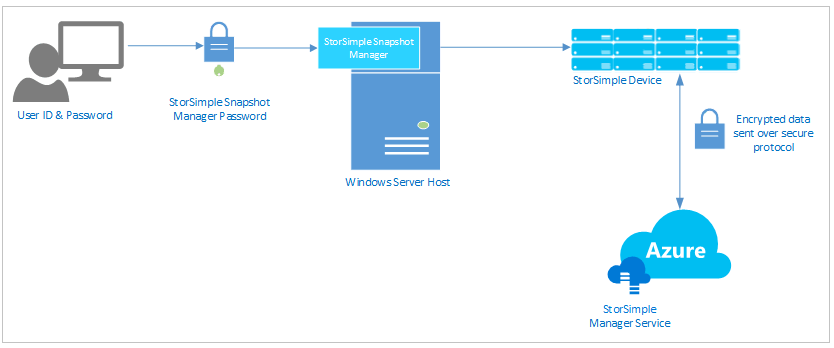
\includegraphics[width=6.5in]{Bilder/storsimple2.png}
\caption{Forenklet bilde av sikkerheten til StorSimple. (Dataencryption, 2016)}
\end{figure}

\paragraph{} Ofte er Microsoft og Sky tjenester koblet med svak sikkerhet. Mange brukere og kunder velger andre former for datalagring som følge av det faktum at Sky tjenester ikke er av den sikreste metoden å lagre data på. I midlertid, står en hybrid sky løsning for å løse dette. Med en slik tjeneste får Katoplast muligheten til å lagre sine sensitive data lokalt på huset, som kun de har tilgang til og som kun de har muligheten til å administrere. Med en slik mulighet blir mange av de bekymringene knyttet til sky lagring løst. Som Figur 5.1 viser så er StorSimple en svært beskyttet løsningen hvor det ikke bare kreves sterke og avanserte passord, men at data og informasjon først blir kryptert og skjult, før de sendes gjennom en sikret internett protokoll. Dette gjøres for å mest mulig sikre brukernes data fra angrep. 
\footnote{https://docs.microsoft.com/en-us/azure/storsimple/storsimple-security}

\subsection{Ulemper med StorSimple}
\paragraph{} StorSimple har mange funksjoner og tjenester ved seg som kan være til fordel for både små og store bedrifter. I midlertid, er ikke StorSimple et helt perfekt system og har en rekke ulemper ved seg. Med betraktning på Katoplast sine muligheter og begrensninger har gruppen kommet frem til en rekke ulemper som kan være interessant for Katoplast å vite og forstå.

\paragraph{} Først og fremst, et av de største ulempene med StorSimple, som med andre hybride løsninger, er at løsningen er dyr og utgjør en bemerkelsesverdig belastning for den økonomiske tilstanden til Katoplast. Med en prislapp på over 140 000 kr årlig, kan StorSimple utgjøre et problem for Katoplast sin økonomi. Selv om Microsoft har lagt et merkbart fokus for å muliggjøre sine løsninger for små bedrifter, er deres hybride skytjenester ikke av det billigste laget. Tjenestene er relative nye og er som følge av dette også kostbare. Det er mulig for Katoplast å få tilpasset løsningene og muligens få begrenset prisen. Foreløpig er prisen likevel høy.

\paragraph{} Den hybride løsningen til Microsoft fokuserer på å fikse mange av de bekymringene som brukere har knyttet til å lagre sensitiv data på et eksternt sted over internett. Likevel er det slik at Microsoft opplever mange former for datakriminalitet og de hybride løsningene kan oppleve å bli utsatt for slike angrep på lik linje med de vanlige sky løsningene. 
\footnote{http://www.eweek.com/cloud/microsoft-azure-flaw-exposed-rhel-virtual-machines-to-hacking-risk}

\paragraph{} En tredje ulempe med Microsoft er at de fra tid til annen opplever aggressive angrep fra enten hackere eller DDOS-angrep, som kan føre til at servere og ytelsen på Microsoft sine tjenester påvirkes. Som en konsekvens av dette kan tjenestene og serverne oppleve nedetid, og dette bør være en faktor som spiller inn dersom Katoplast skulle ønske å skifte over til Microsoft sin løsning. Likevel, er dette noe som skjer sjeldent og når det skjer så har det som oftest ikke alvorlige følger.
\footnote{http://www.networkworld.com/article/2224155/microsoft-subnet/microsoft-admits-to-being-hacked-too.html}

\subsection{StorSimple Verdict} 
\begin{figure}[H]
\centering
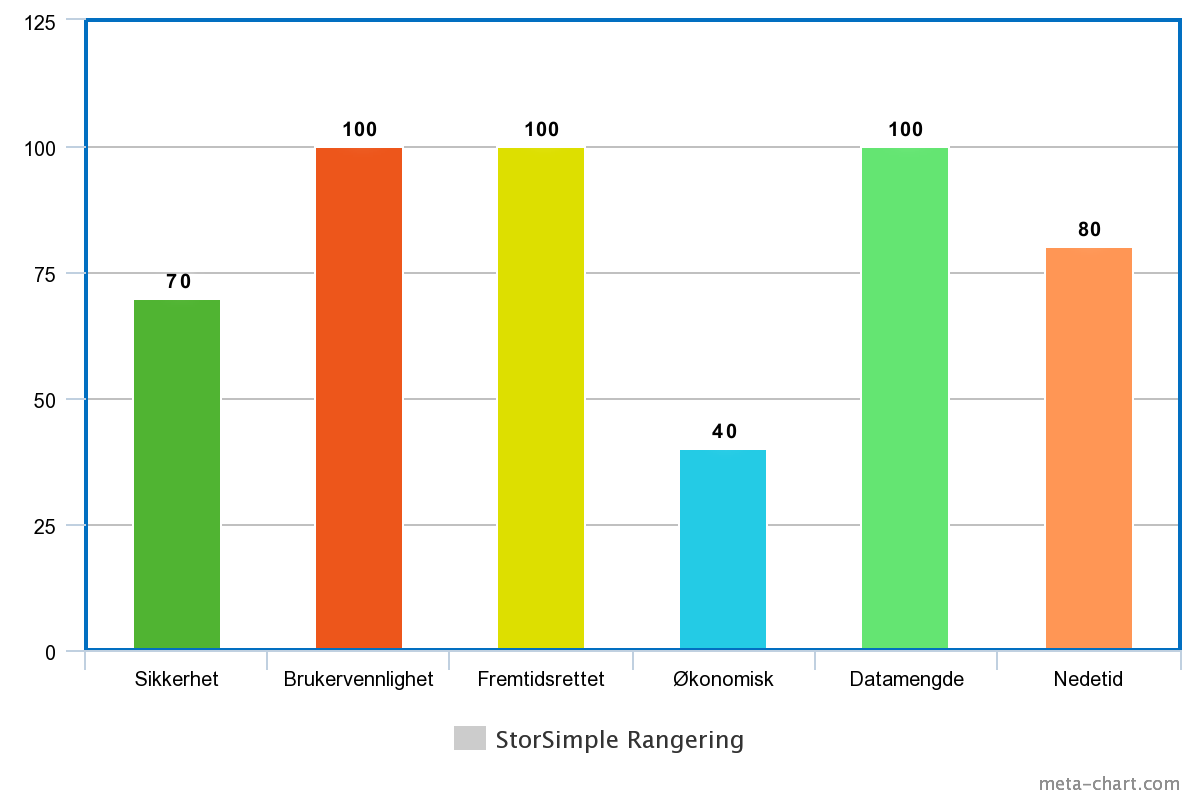
\includegraphics[width=6.5in]{Bilder/chart.png}
\caption{StorSimples rangering etter arbeidskravene.}
\end{figure}

\paragraph{} Dataene over tar i betraktning arbeidskravs analysen og gruppen rangerer StorSimple slik som figur 5.1 viser. Dette er gruppens vurdering av StorSimple ut i fra de kravene som er stilt og basert på resultatene og informasjonen som er samlet inn.

\section{VMware - Hybrid} 
\subsection{Fordeler med VMware}
\paragraph{} Som en av de senere organisasjonene til å introdusere Sky tjenester til omverdenen, har VMware fra tidligere etablert seg godt innenfor ytelse og pålitelighet. Med deres lange erfaring innenfor programvare utvikling som strekker seg helt fra 1998, har VMware håndtert overføring til å tilby skylagring av aller høyeste nivå på en positiv måte. Dette gjør VMware til en fordel når det gjelder fremtidig teknologi, ettersom de er raske med å etablere seg og har lang erfaring med programvareutvikling. 
\footnote{http://www.vmware.com/company.html}
\footnote{http://www.nytimes.com/2009/08/31/technology/business-computing/31virtual.html?pagewanted=2\&\_r=2\&partner=rss\&emc=rss}

\paragraph{} En vesentlig fordel med VMware er at de tilbyr brukerne sine å kontrollere alle tjenester gjennom deres  "vCloud Suite" platform. Dette gjør det lettere for brukere å administrere deres sky tjenester, samtidig som det gir forbedret kontroll over brukernes kjøp. Tjenesten assisterer også med å oppgradere programvare og verktøy, eller eventuelt nedgradere disse dersom en oppdatering skulle vise seg å være problematisk.
\footnote{http://www.vmware.com/products/vcloud-suite.html}

\paragraph{} VMware har, som tidligere nevnt, flere års erfaring med utvikling av programvare og applikasjoner. Med dette tilbyr de brukerne sine et bredt spekter av ressurser, funksjoner, verktøy og innebygde prosesser som hjelper med installasjon, oppsett og drifting av serverne, og ikke minst hjelpe kundene sine innenfor andre bruksområder. Samtidig, tar disse funksjonene seg også av de administrative oppgavene som Katoplast ofte føler tar en omfattende del av arbeidet når det gjelder deres servere. 
\footnote{http://www.vmware.com/products/vcloud-suite.html}

\paragraph{} Ikke minst, er disse programvarene en del av å opprettholde sikkerheten på den hybride løsningen. I motsetning til Microsoft så er ikke VMware i like stor grad under angrep av hackere. Dette gjør at VMware scorer høyere på sikkerhet enn det Microsoft gjør. I tillegg så er en hybrid løsning skapt for å sikre de sensitive opplysningene til en bedrift, ved at kun bedriften har tilgang til den private skyen.
\footnote{http://www.vmware.com/products.html}

\paragraph{} En positiv fordel med VMware sin løsning er at kundene som benytter seg av sitt kjøp, behøver kun å måtte betale for den dataen de benytter seg av og ikke noe mer. Dette er et omfattende steg mot en lettere økonomisk hverdag for katoplast når det gjelder servere. Med et slikt alternativ trenger ikke bedriften å bekymre seg for å måtte betale for ubrukte data. Katoplast betaler for 1,4 mer terabyte (TB) enn det de behøver, med deres nåværende løsning. Dette er overdrevent ettersom bedriften kun benytter seg av 500 gigabyte med lagringsplass!
\footnote{http://www.vmware.com/cloud-services/pricing-guide.html}

\begin{figure}[H]
\centering
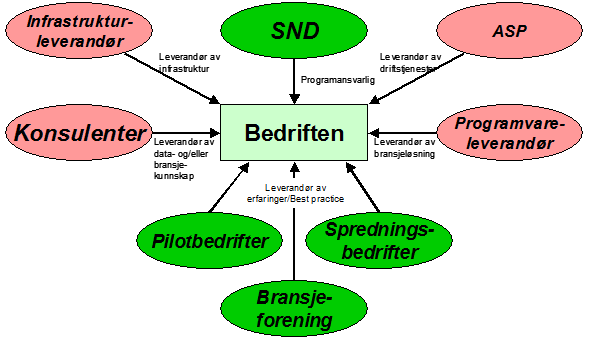
\includegraphics[width=6.5in]{Bilder/ss.png}
\caption{Nettverk av aktorer. (Christensen,2003, s.16)}
\end{figure}

\paragraph{} Som tidligere nevnt så tilbyr VMware ikke direkte sine løsninger til kunder, men gjør dette heller gjennom ulike partner nettverk, såkalte aktører. Hver av disse nettverkene bidrar med ressurser og verktøy til VMware, som hjelper med å danne de ulike løsningene som de tilbyr sine kunder. Samme opplegget kommer Katoplast til å oppleve når de må benytte seg av flere ulike aktører for deres server løsning. Fordelen med VMware og Microsoft er at disse aktørene deles heller i en, hvor leverandøren av løsningen også står ansvarlig for andre deler av prosessen. 
\footnote{http://www.tomsitpro.com/articles/hybrid-cloud-providers-comparison,2-841.html}
\footnote{https://www.vmware.com/partners.html}

\paragraph{} Figur 5.2 viser hvordan dette nettverket av aktører fungerer, og hvordan en bedrift får sine tjenester fra mange, ulike sider. VMware derimot inkluderer alle disse tjenestene i 1 pakke, hvor de samarbeider med ulike aktører, samt danner sine egne programmer. Dermed slipper Katoplast å måtte bekymre seg over å hyre inn egne konsulenter, programvare leverandører eller annet. De fleste hybride løsningene tilbyr dette i en helhetlig pakke som de gir til sine bedrifter, og med VMware sitt store partner nettverk er mulighetene enda større enn med andre løsninger.

\subsection{Ulemper med VMware}
\paragraph{} En ulempe med VMware er at deres forretningsmodell når det kommer til hybride løsninger er rotete. Dette gjør at kunder og brukere ofte ikke vet hva de egentlig betaler for og hva de egentlig får ut av de ulike alternativene som VMware tilbyr kundene sine. Dette kan påvirke installasjonen og oppdateringer av de hybride løsningene på en negativ måte. Det kan føre til at kunder benytter seg av feil programvare eller oppgraderer sine programmer uten å vite hva de egentlig gjør.
\footnote{http://marketrealist.com/2014/08/why-emc-vmware-and-pivotal-form-a-unique-business-model/}
\footnote{http://www.tomsitpro.com/articles/hybrid-cloud-providers-comparison,2-841.html}

\paragraph{} En annen ulempe med denne løsningen er at VMware ikke direkte er leverandøren av den hybride tjenesten. VMware er sponset av mange ulike nettverk som brukere må benytte seg av for å få tilgang til de hybride løsningene. Dette kan ofte føre til forvirring blant kunder om hvem de egentlig betaler til og hva de egentlig kjøper.
\footnote{https://www.vmware.com/partners/oem.html}

\paragraph{} Selv om VMware har lagt et betydelig fokus på brukervennlighet, føles det ikke alltid slik. Deres avanserte forretningsmodell og deres partner nettverk gjør det ikke lett for brukerne å forstå hvordan de skal gå frem med å kjøpe tjenestene og hvordan tjenestene helt fungerer. Spesielt når det gjelder kunder som ikke er eksperter innenfor IT-område. Selv om, mange av deres tjenester og produkter har et simplet brukergrensesnitt, påvirkes dette negativt av forretningsmodellen til VMware.

\paragraph{} Som med tidligere Hybride løsninger så er også VMware en relativt dyr løsning for en bedrift som Katoplast. Med en prislapp på litt over 81000 kr årlig, så er løsningen kostbar. Fordelene som følger med er enestående for bedriften, men overskygges av den høye prislappen.
\footnote{https://www.vmware.com/partners/partner-learning.html}

\subsection{VMware Verdict}
\begin{figure}[H]
\centering
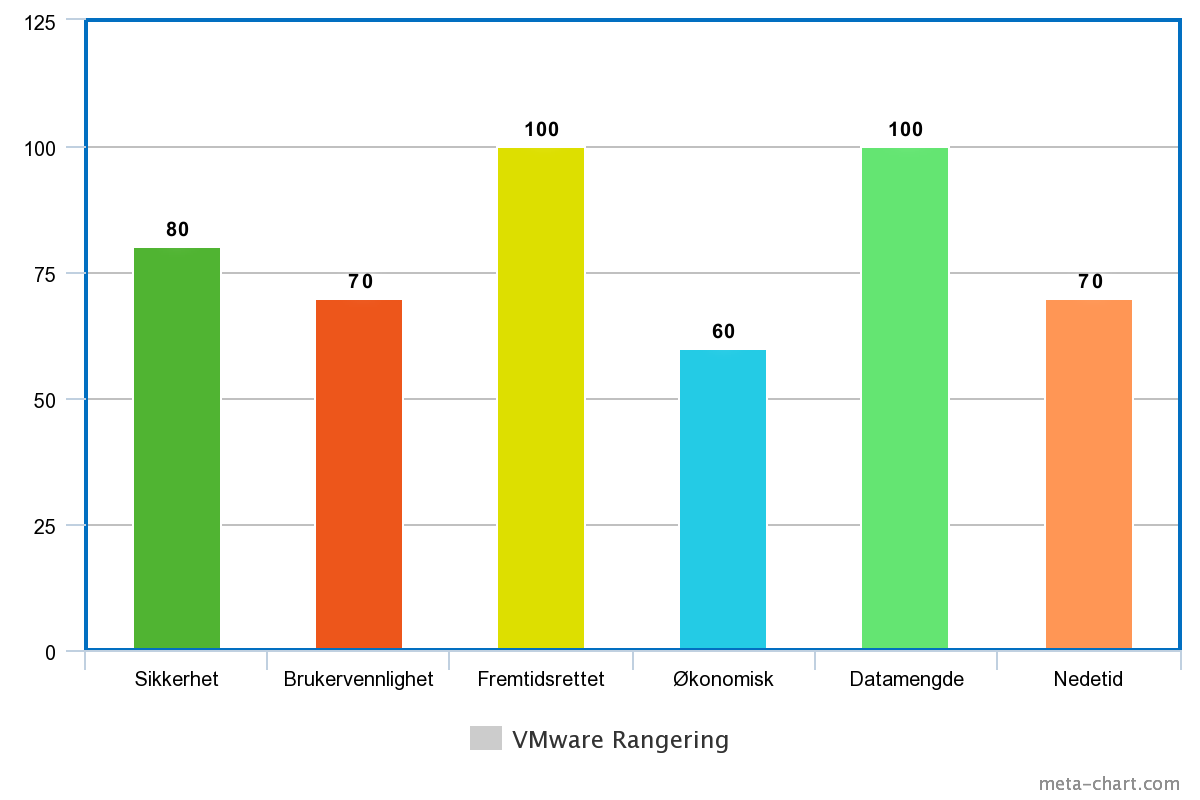
\includegraphics[width=6.5in]{Bilder/chart2.png}
\caption{VMware rangering etter arbeidskravene.}
\end{figure}

\paragraph{} Figure 5.2 viser hvordan prosjektgruppen rangerer VMware sin hybride løsning ut i fra de ulike arbeidskravene som har blitt stilt og ut i fra situasjonsanalysen som ble laget. Gruppen ønsker at Katoplast skal oppleve en helt ny hverdag med de nye hybride løsningene, hvor bedriften slipper å bekymre seg om sikkerheten og de administrative arbeidsoppgavene som må gjøres. VMware sin løsning er økonomisk sett billigere enn andre hybride løsninger.  Med en prislapp på cirka 81 000 kr årlig er løsningen fortsatt dyr, men mange hakk billigere enn andre løsninger. Det positive med VMware sin løsning derimot, er at den tar et godt steg inn i den hybride trenden som preger nye server løsninger. Dersom Katoplast skulle ønske å benytte seg av hybride løsninger er VMware sin løsning det beste startpunktet. 

\chapter{Konklusjon}
\paragraph{} Konklusjonen er det siste kapittelet i rapporten, og kapittelet oppsummerer det prosjektgruppen har funnet ut av gjennom analysene og forskningen som er blitt gjennomført. Konklusjonen vil også presentere en anbefaling for en løsning til bedriften som de kan få nytte av. 

\section{Anbefaling}
\paragraph{} Prosjektet har tatt for seg ulike serverløsninger for både interne, eksterne og hybride servere -og har analysert muligheter innenfor hver av disse områdene. Med et fokus på kravspesifikasjonene og avgrensningene som bedriften la ned, har prosjektgruppen klart å analysere og rapportere om ulike løsninger som kan løse Katoplast sitt server problem. Det er imidlertid slik at ikke alle disse løsningene er perfekte, og hver og en av disse har sine fordeler og ulemper som kan være interessante for Katoplast å forstå.

\paragraph{} Med tanke på økonomien vil Katoplast få betraktelig mindre kostnader når det gjelder kjøp og drifting av serverne. PC Hjelp AS tilbyr en server for 10 072 kr og konsulent arbeid for 3 160 kr. I motsetning til Borg Svakstrøm som tilbød serverne sine for 84 900 kr samt installasjon og oppsett av serverne på 7 dager for 41 000 kr. Dette er en merkbar forskjell på prisene. Dersom Katoplast ikke ønsker å fjerne sine gamle servere, foreslår prosjektgruppen at Katoplast heller beholder de gamle serverne sine -og benytter disse som backup servere, mens de nye serverne fra PC Hjelp AS benyttes som standard servere.

\paragraph{} Etter en grundig evaluering av alle løsningene, en evaluering av katoplast sin nåværende situasjon, deres ønsker og de arbeidskravene som er stilt for prosjektet så har gruppens valg falt på PC Hjelp AS. PC Hjelp AS tilbyr gruppen en svært rimelig løsning som er billig, effektiv og som møter ønskene til katoplast. Dette er en intern server som PC Hjelpen tilbyr med cirka 2TB lagringsplass. Operativ Systemet er Windows, som er nettopp det Katoplast ønsket. I tillegg til dette tilbyr PC Hjelp AS konsulent-arbeid for oppsett av serveren. Dette vil ta mellom 1-2 dager og vil koste Katoplast 3 160 kr. Valget til gruppen falt på denne løsningen ettersom den var svært rimelig for økonomien, samtidig som at det er en intern server noe Katoplast hadde som et sterkt ønske. 

%%===========Attachments==============

\begin{thebibliography}{999}

\bibitem{1} Christensen, Bo Hjort.(2003). \textit{Effektiv anvendelse av IKT : elektronisk forretningsdrift}. Oslo : SND, BIT-programmet.

\bibitem{} Sanders, James. (2014). Hybrid cloud: What it is, why it matters. \textit{ZDnet}. Hentet fra: http://www.zdnet.com/article/hybrid-cloud-what-it-is-why-it-matters/

\bibitem{} Kirsch, Brian. (2015). 6 Hybrid Cloud Providers Compared. \textit{Tom's IT Pro}. Hentet fra: http://www.tomsitpro.com/articles/hybrid-cloud-providers-comparison,2-841.html

\bibitem{} Warner, Tim. (2015). Microsoft Nano Server: Everything you need to know. \textit{Pluralsight}. Hentet fra: https://www.pluralsight.com/blog/it-ops/microsoft-nano-server-announced. 

\bibitem{} Laudon, Kenneth C., \& Laudon, Jane P.(2016). \textit{Management Information Systems, Managing the Digital Firm}.Pearson Education.

\bibitem{} Winslow, Dana. (2016). \textit{Why You Need a Local Testing Server (and How To Do It)}. Hentet fra: http://www.dwuser.com/education/content/why-you-need-a-testing-server-and-how-to-do-it/

\bibitem{} Ramachandran, Udaiappa. (2013). \textit{The Pros and Cons of Cloud Storage}.
Hentet fra: http://www.episerver.com/learn/resources/blog/udaiappa-ramachandran/the-pros-and-cons-of-cloud-storage/

\bibitem{} Davis, Kevin. (2014). \textit{Pros and Cons: Digging into Amazon Web Services}
Hentet fra: https://npifinancial.com/blog/pros-and-cons-digging-into-amazon-web-services/

\bibitem{} Vaughan-Nichols, Steven J. (2015). \textit{How Amazon Web Services crashed and rose again}
Hentet fra: http://www.zdnet.com/article/how-amazon-web-services-crashed-and-rose-again/

\bibitem{} Hambrick, Scott. (2015). \textit{Amazon Web Services Storage: Pros and Cons for Document Management}
Hentet fra: https://www.datastorageinc.com/blog/amazon-web-services-storage-pros-and-cons-for-document-management

\bibitem{} Hernandez, Pedro. (2016). \textit{Microsoft Azure Flaw Exposed RHEL Virtual Machines to Hacking Risk}
Hentet fra: http://www.networkworld.com/article/2224155/microsoft-subnet/microsoft-admits-to-being-hacked-too.html

\bibitem{} Smith, Ms. (2013, 25.04). Microsoft admits to being hacked too. \textit{Networkworld}
Hentet fra: http://www.networkworld.com/article/2224155/microsoft-subnet/microsoft-admits-to-being-hacked-too.html

\bibitem{} Shields, Anna. (2014). \textit{Why EMC, VMware, and Pivotal form a unique business model}
Hentet fra: http://marketrealist.com/2014/08/why-emc-vmware-and-pivotal-form-a-unique-business-model/

\bibitem{} Goldstein, Phil. (2017). Microsoft Warns that Virtual Machines Could Be Turned into Botnets. \textit{Biztechmagazine}. 
Hentet fra: http://www.biztechmagazine.com/article/2017/01/microsoft-warns-hacked-virtual-machines-are-very-real-threat

\bibitem{} Millman, Rene. (2016). Microsoft update left Azure Linux virtual machines open to hacking. \textit{SC Magazine UK}. 
Hentet fra: https://www.scmagazineuk.com/microsoft-update-left-azure-linux-virtual-machines-open-to-hacking/article/575472/

\bibitem{} Davis, Kevin. (2014). \textit{Pros and Cons: Digging into Amazon Web Services}. 
Hentet fra: https://npifinancial.com/blog/pros-and-cons-digging-into-amazon-web-services/

\paragraph{}\textbf{Bilder:}

\bibitem{}Msazurelogo. Hentet fra https://www.cristie.com/move/clonemanager-in-microsoft-azure/

\bibitem{} Amazon Web Services Immersion Day. Hentet fra https://bruintech.ucla.edu/events/2016-06-16/amazon-web-services-immersion-day

\bibitem{}Roadmap. Hentet fra http://www.cbronline.com/news/cloud/google-reveals-hybrid-cloud-plans-with-openstack-4863087/

\bibitem{} StorSimple. 
Hentet fra: https://azurecomcdn.azureedge.net/cvt-5d7b29713a4471c09f76f0526e9a341f048cd34f90636a43a421f075efb78f10/images/page/services/storsimple/diagram.png

\bibitem{}VMware. Hentet fra http://www.stablenet.net/solutions/cloud-computing/hybrid-cloud/

\bibitem{}Dataencryption. Hentet fra https://docs.microsoft.com/en-us/azure/storsimple/storsimple-security

\bibitem{}Hybrid Cloud. Hentet fra http://www.zdnet.com/article/vmwares-vision-and-roadmap-for-hybrid-cloud/
\end{thebibliography}
\include{Vedlegg/ordre}
\appendix

\chapter{Vedlegg 1}
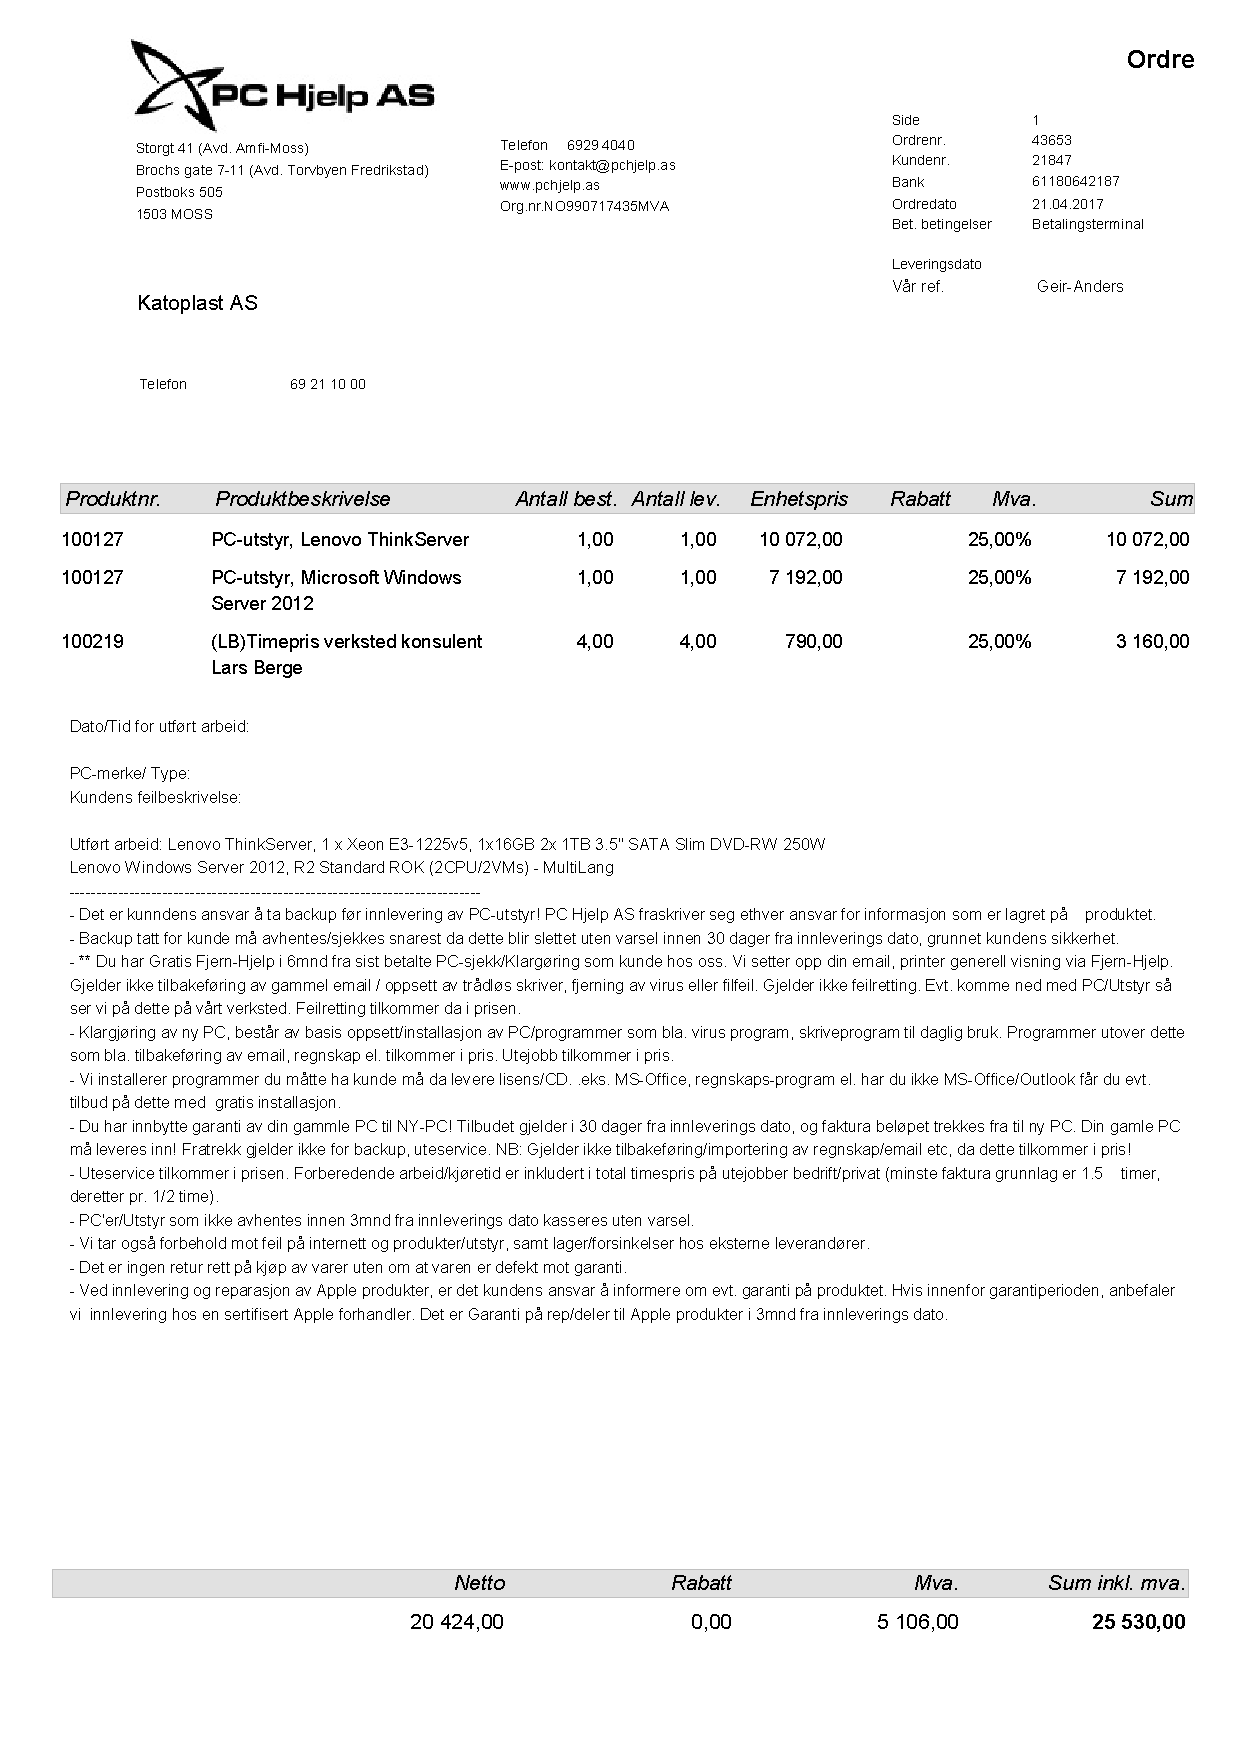
\includepdf[scale=0.9999]{ordre.PDF}

\chapter{Vedlegg 2}
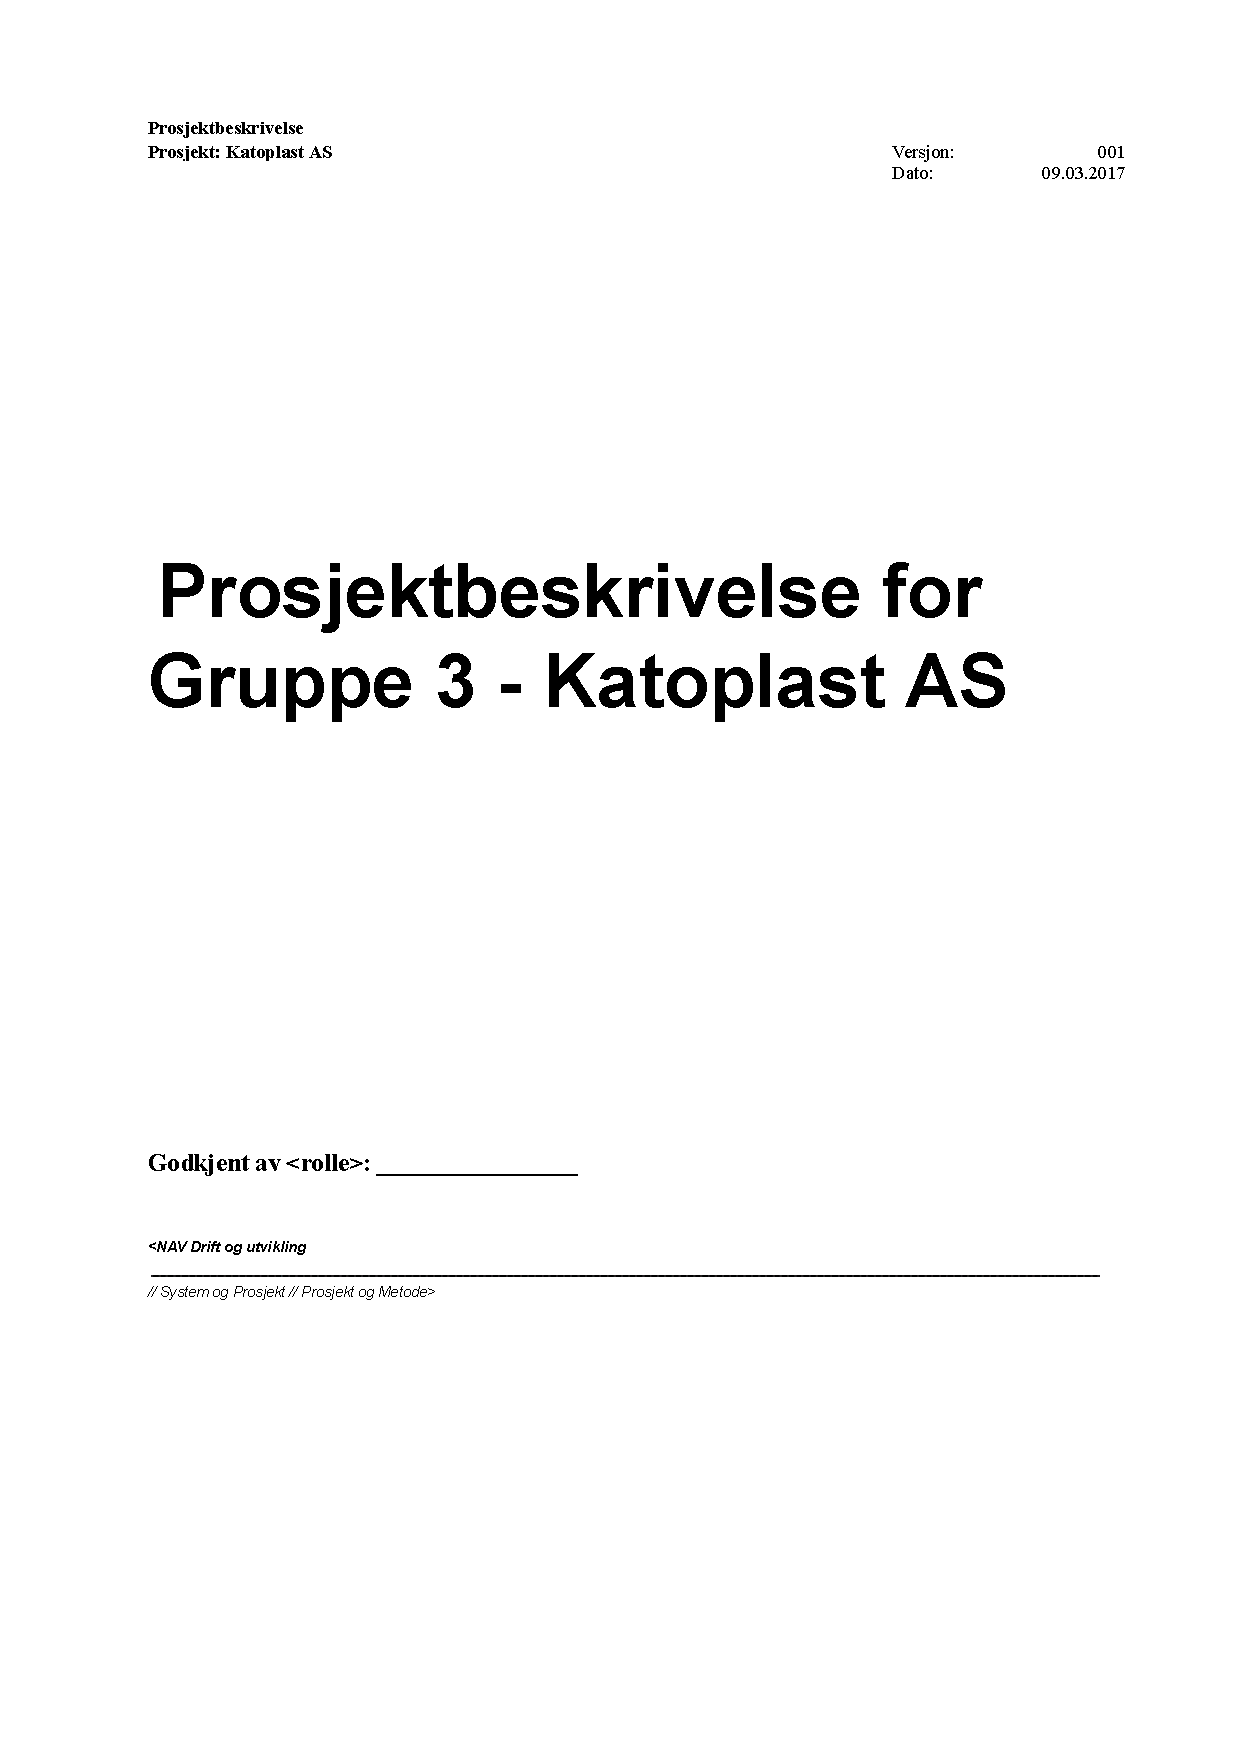
\includepdf[pages=1-14, scale=0.9999]{forprosjektrapport.pdf}

\chapter{Vedlegg 3}
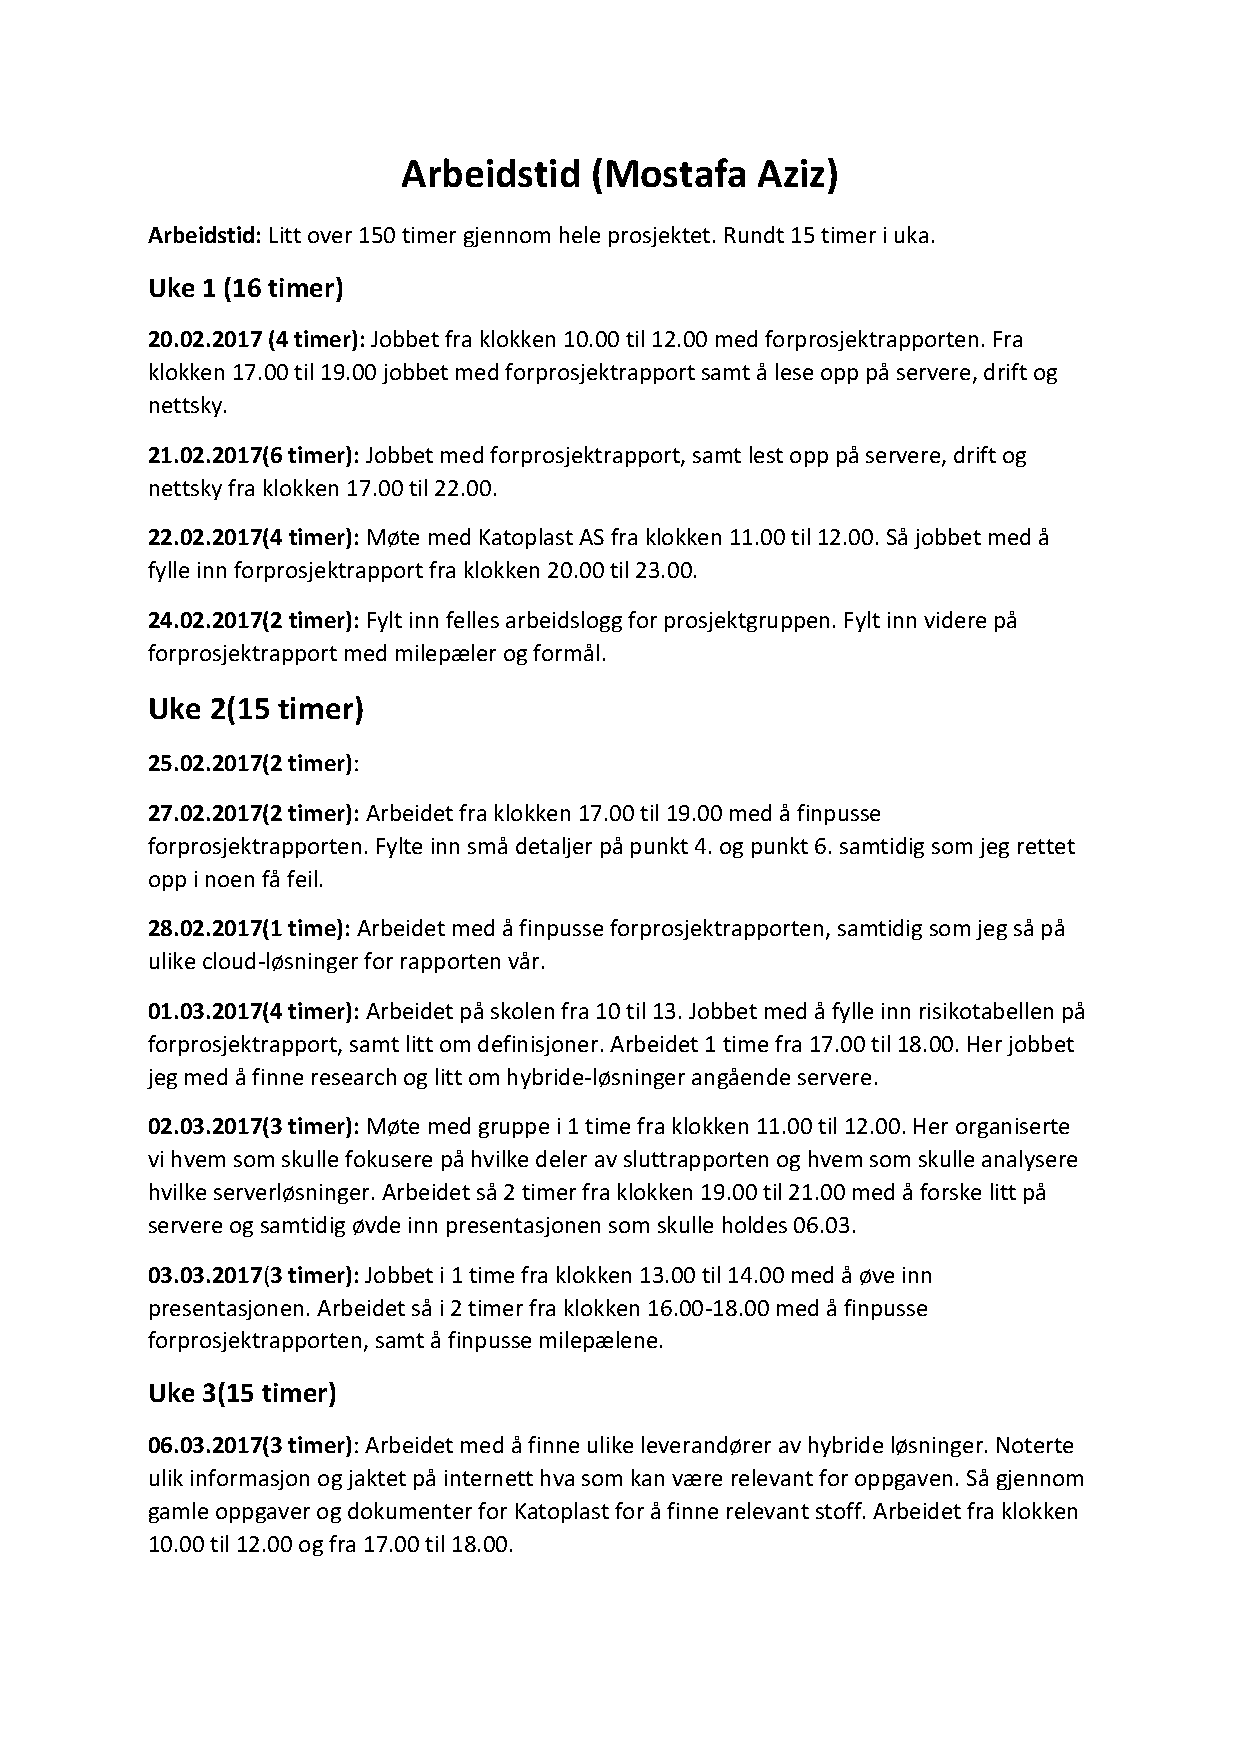
\includepdf[pages=1-5, scale=0.9999]{mostarbeid.pdf}
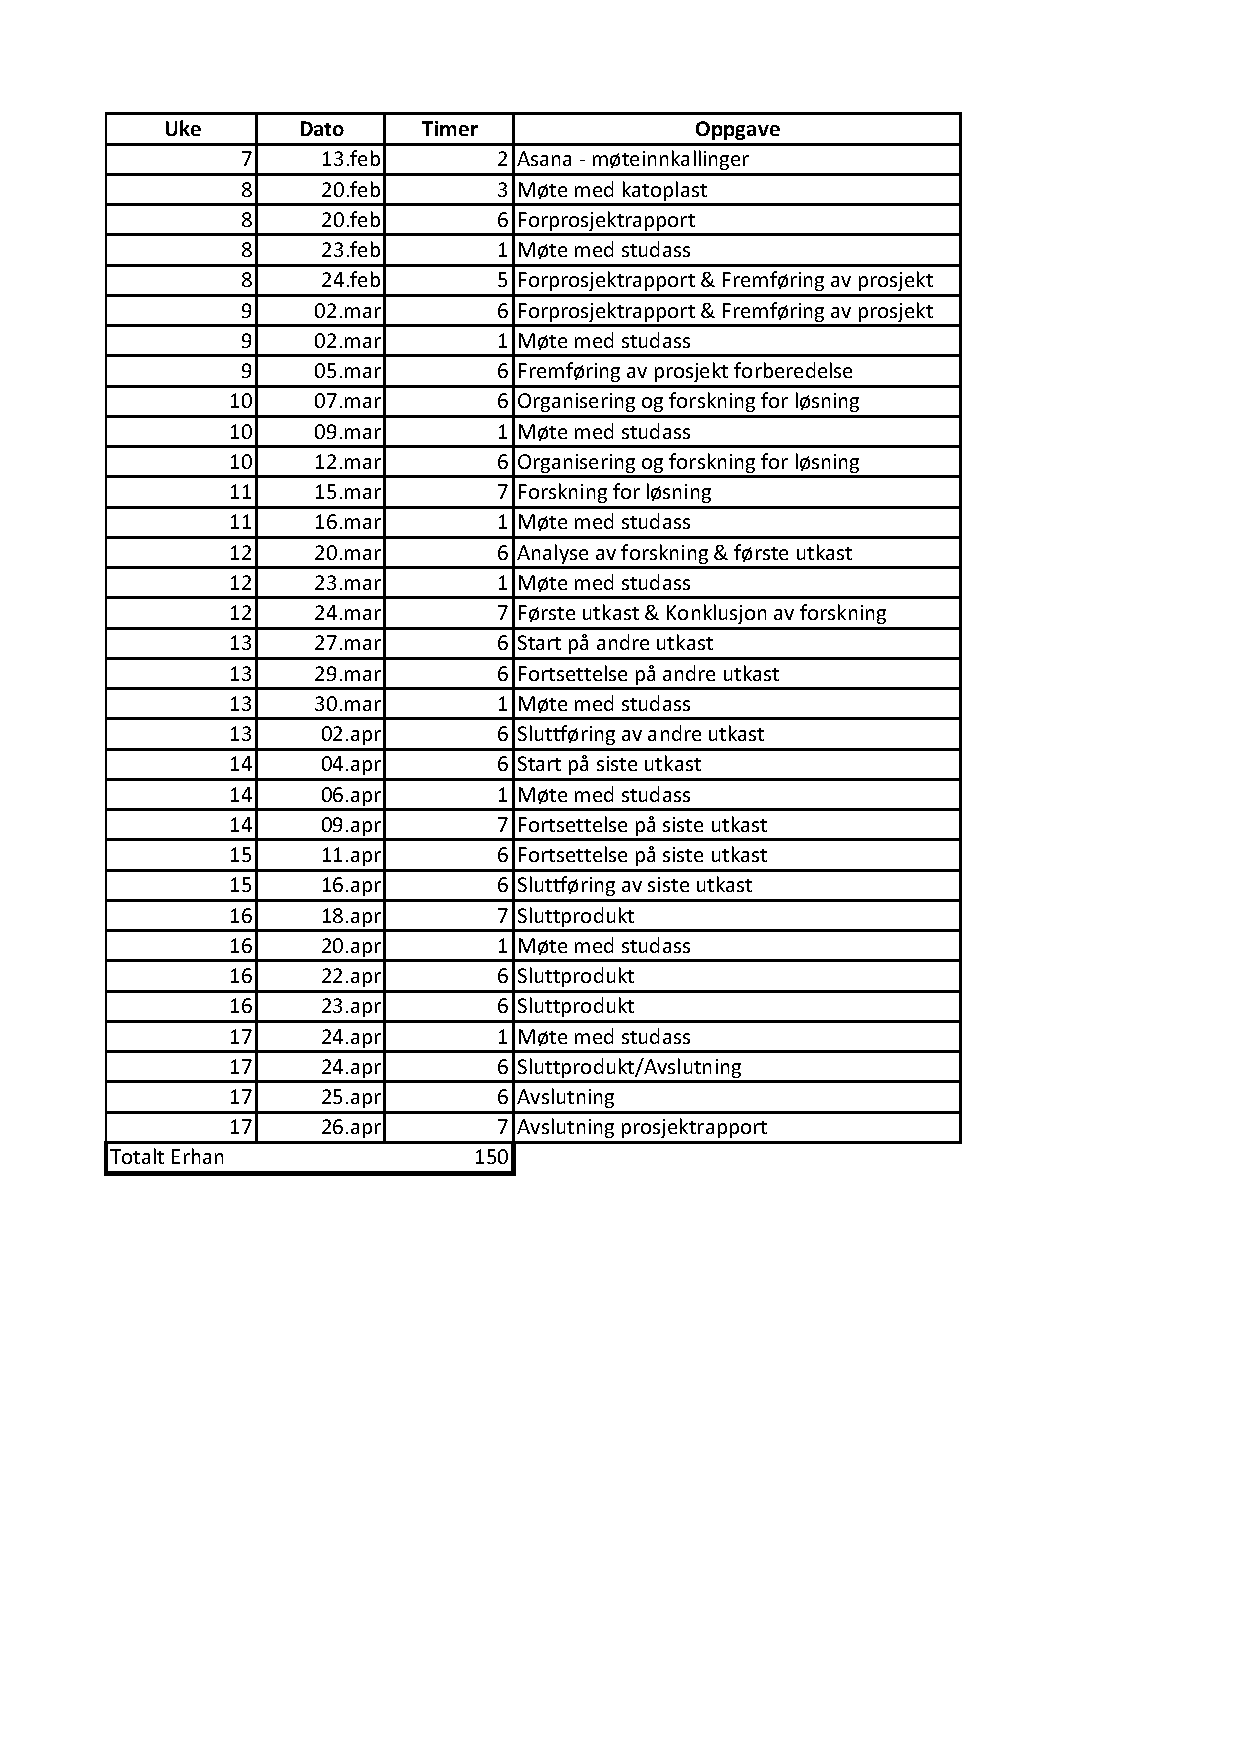
\includepdf[scale=0.9999]{Timelogg.pdf}
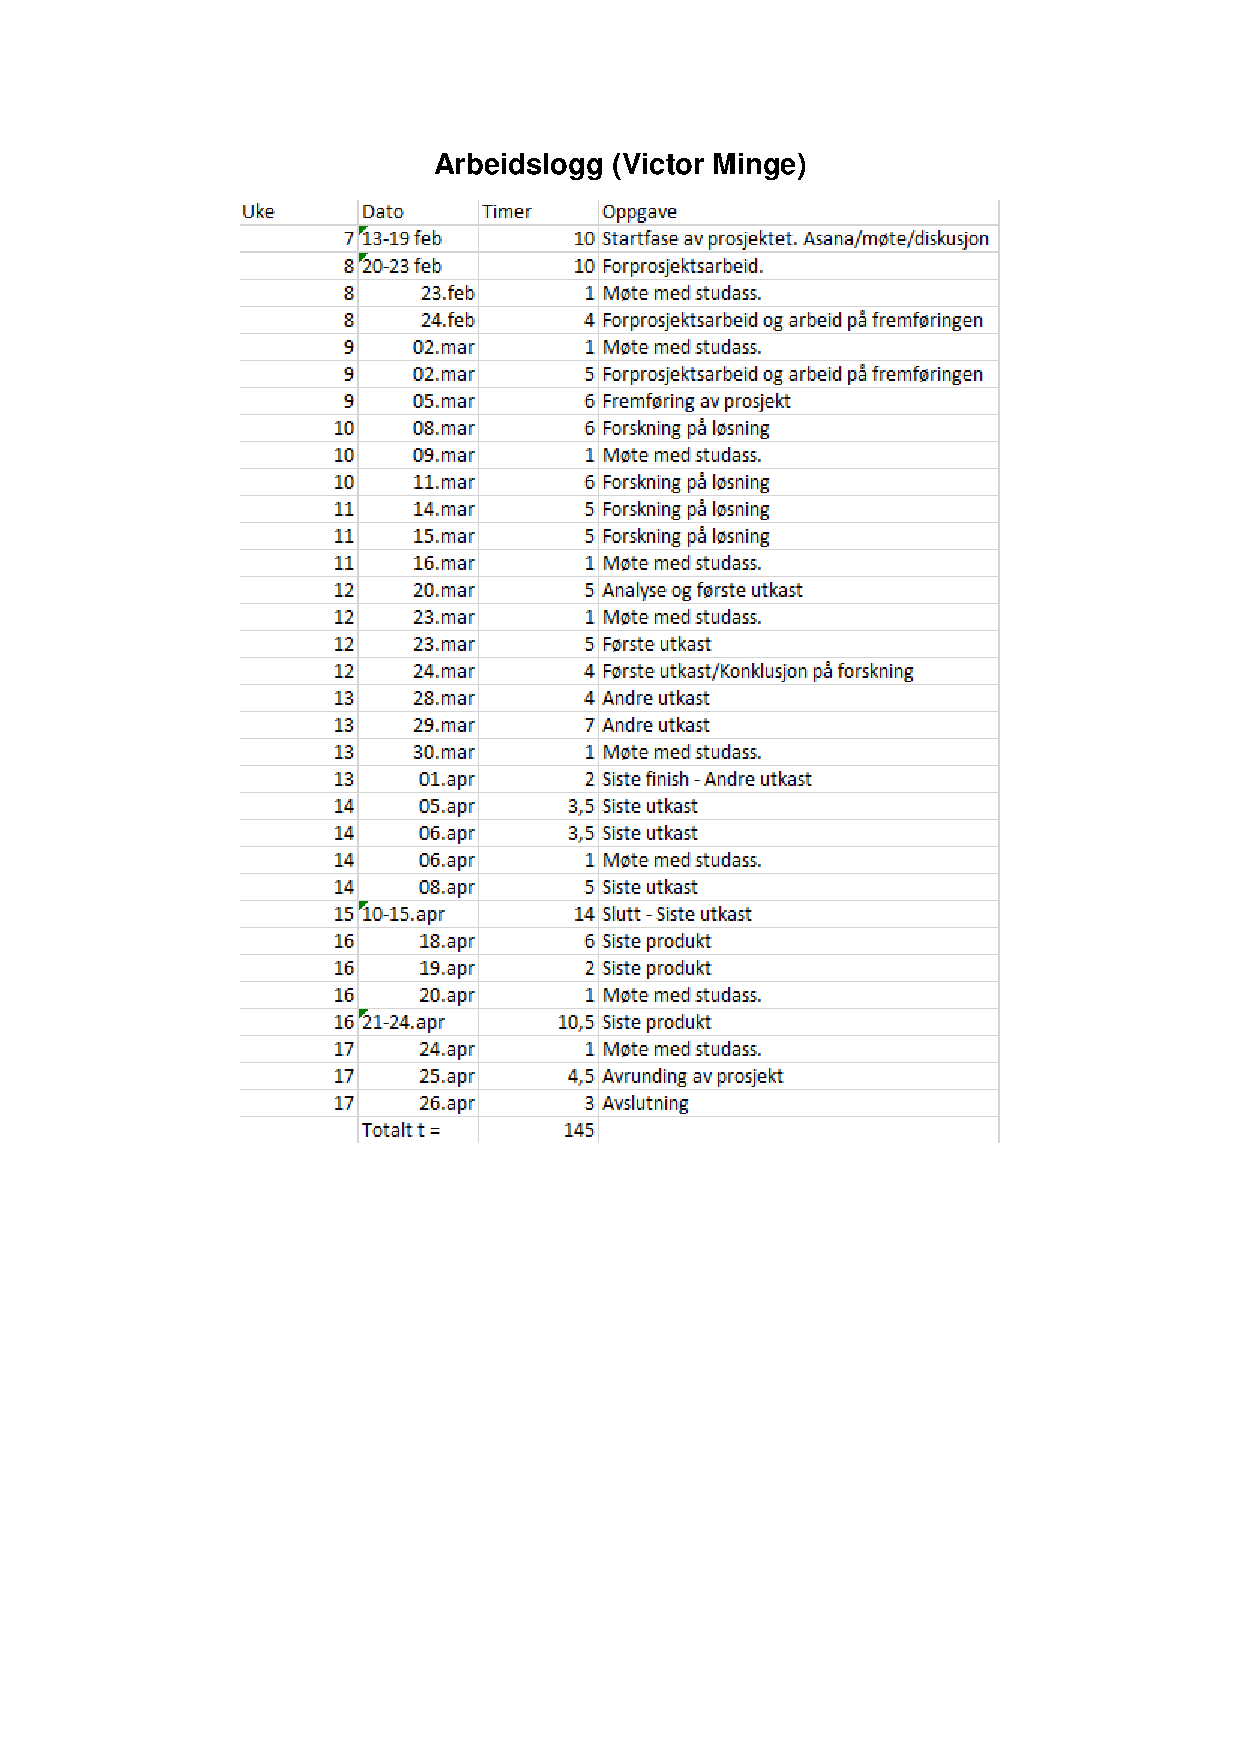
\includepdf[scale=1]{Arbeidslogg.pdf}
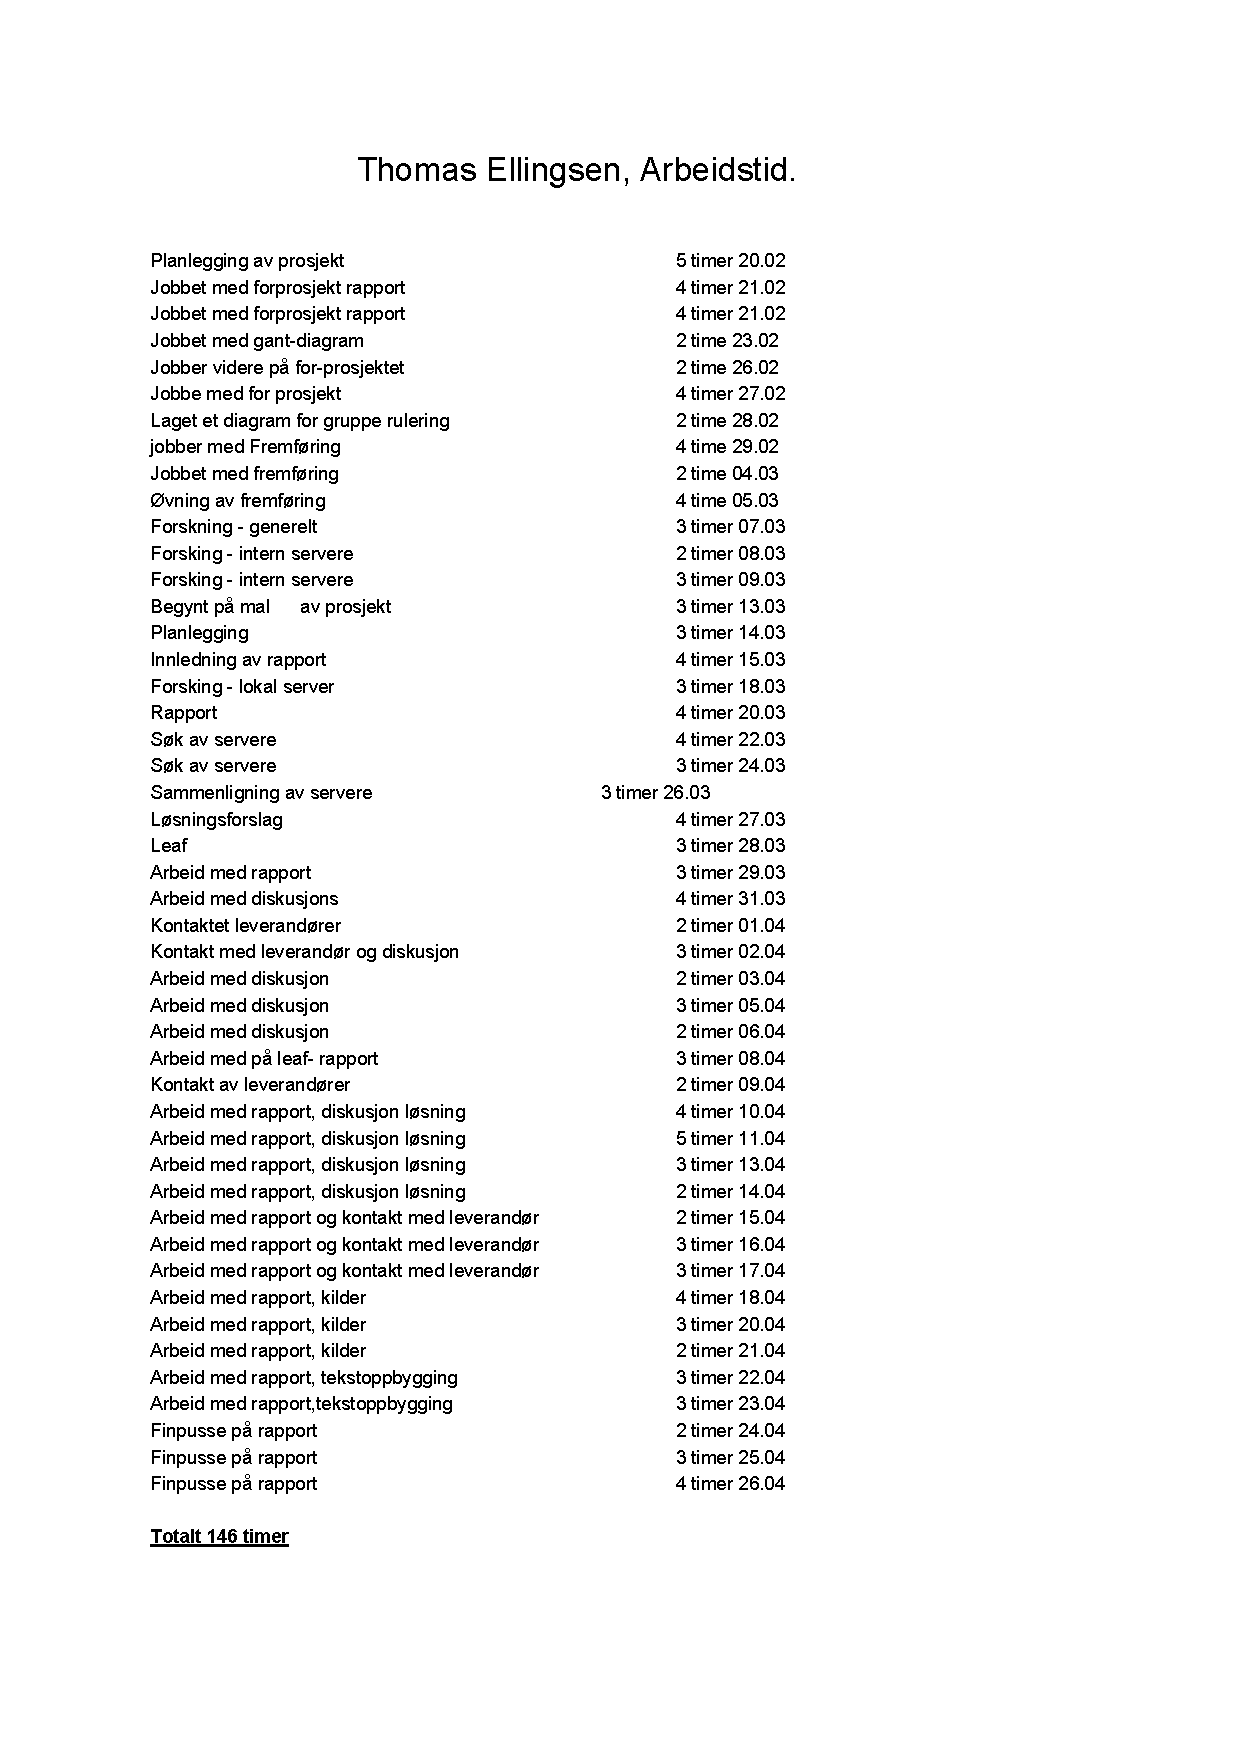
\includepdf[scale=1]{thomastimer.pdf}

\chapter{Vedlegg 4}
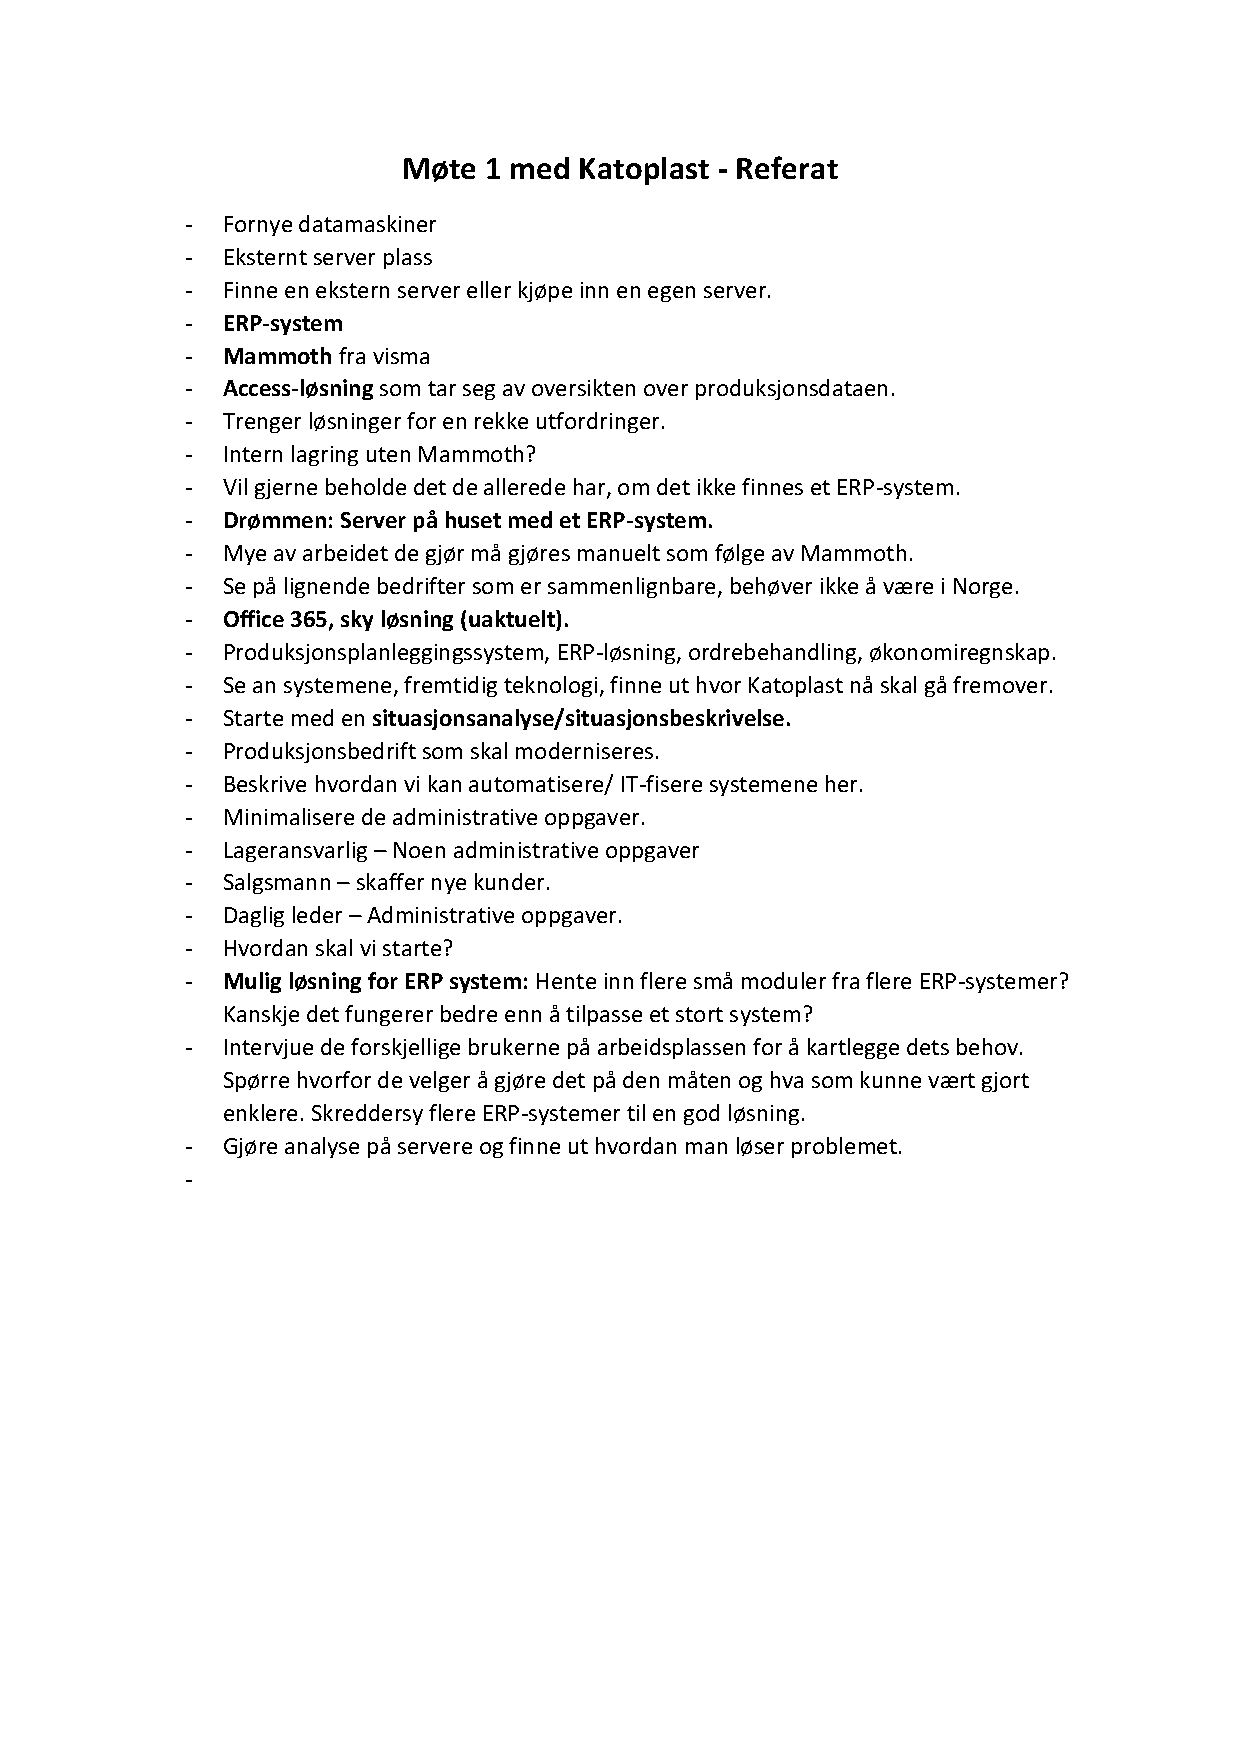
\includepdf[scale=1]{mote1.pdf}

\chapter{Vedlegg 5}
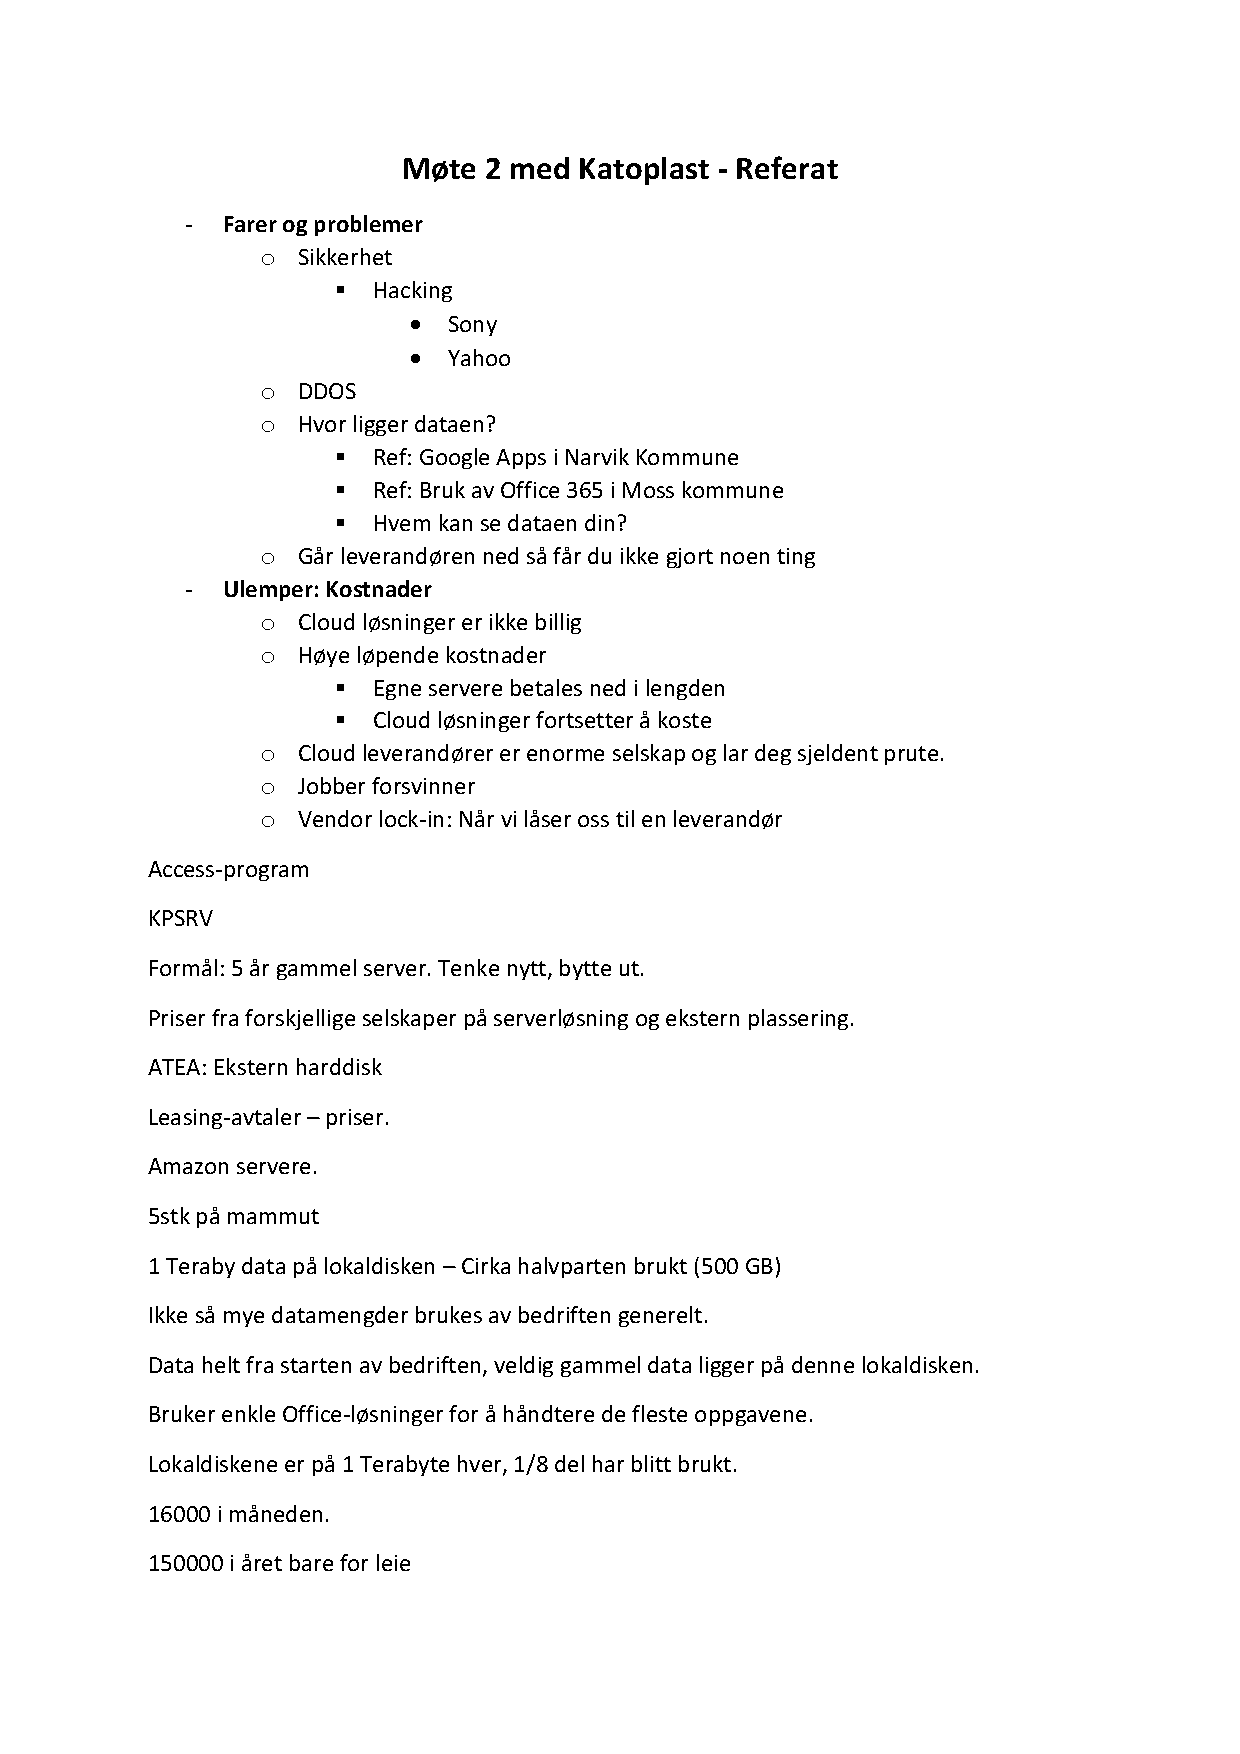
\includepdf[scale=1]{mote2.pdf}

\chapter{Vedlegg 6}
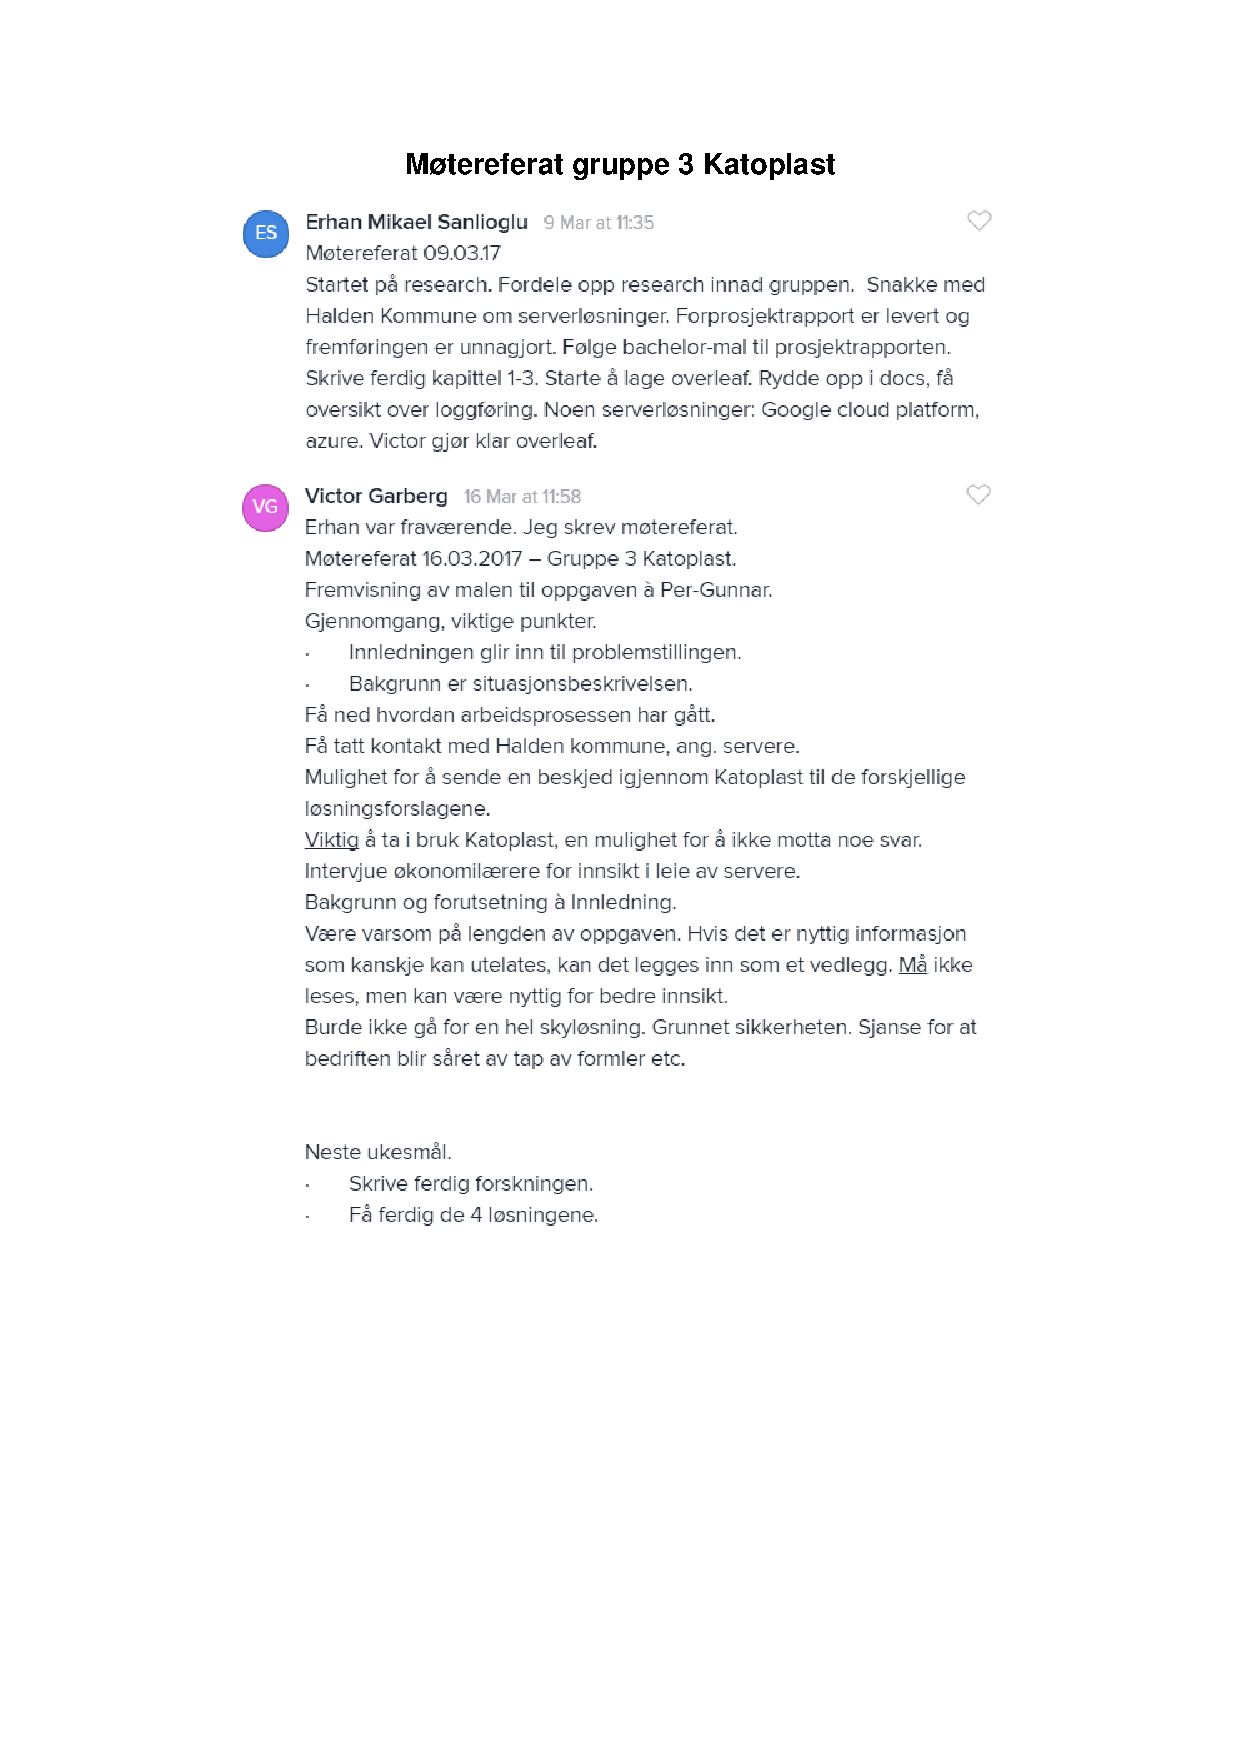
\includepdf[pages=1-3, scale=0.9999]{moter.pdf}

\chapter{Vedlegg 7}
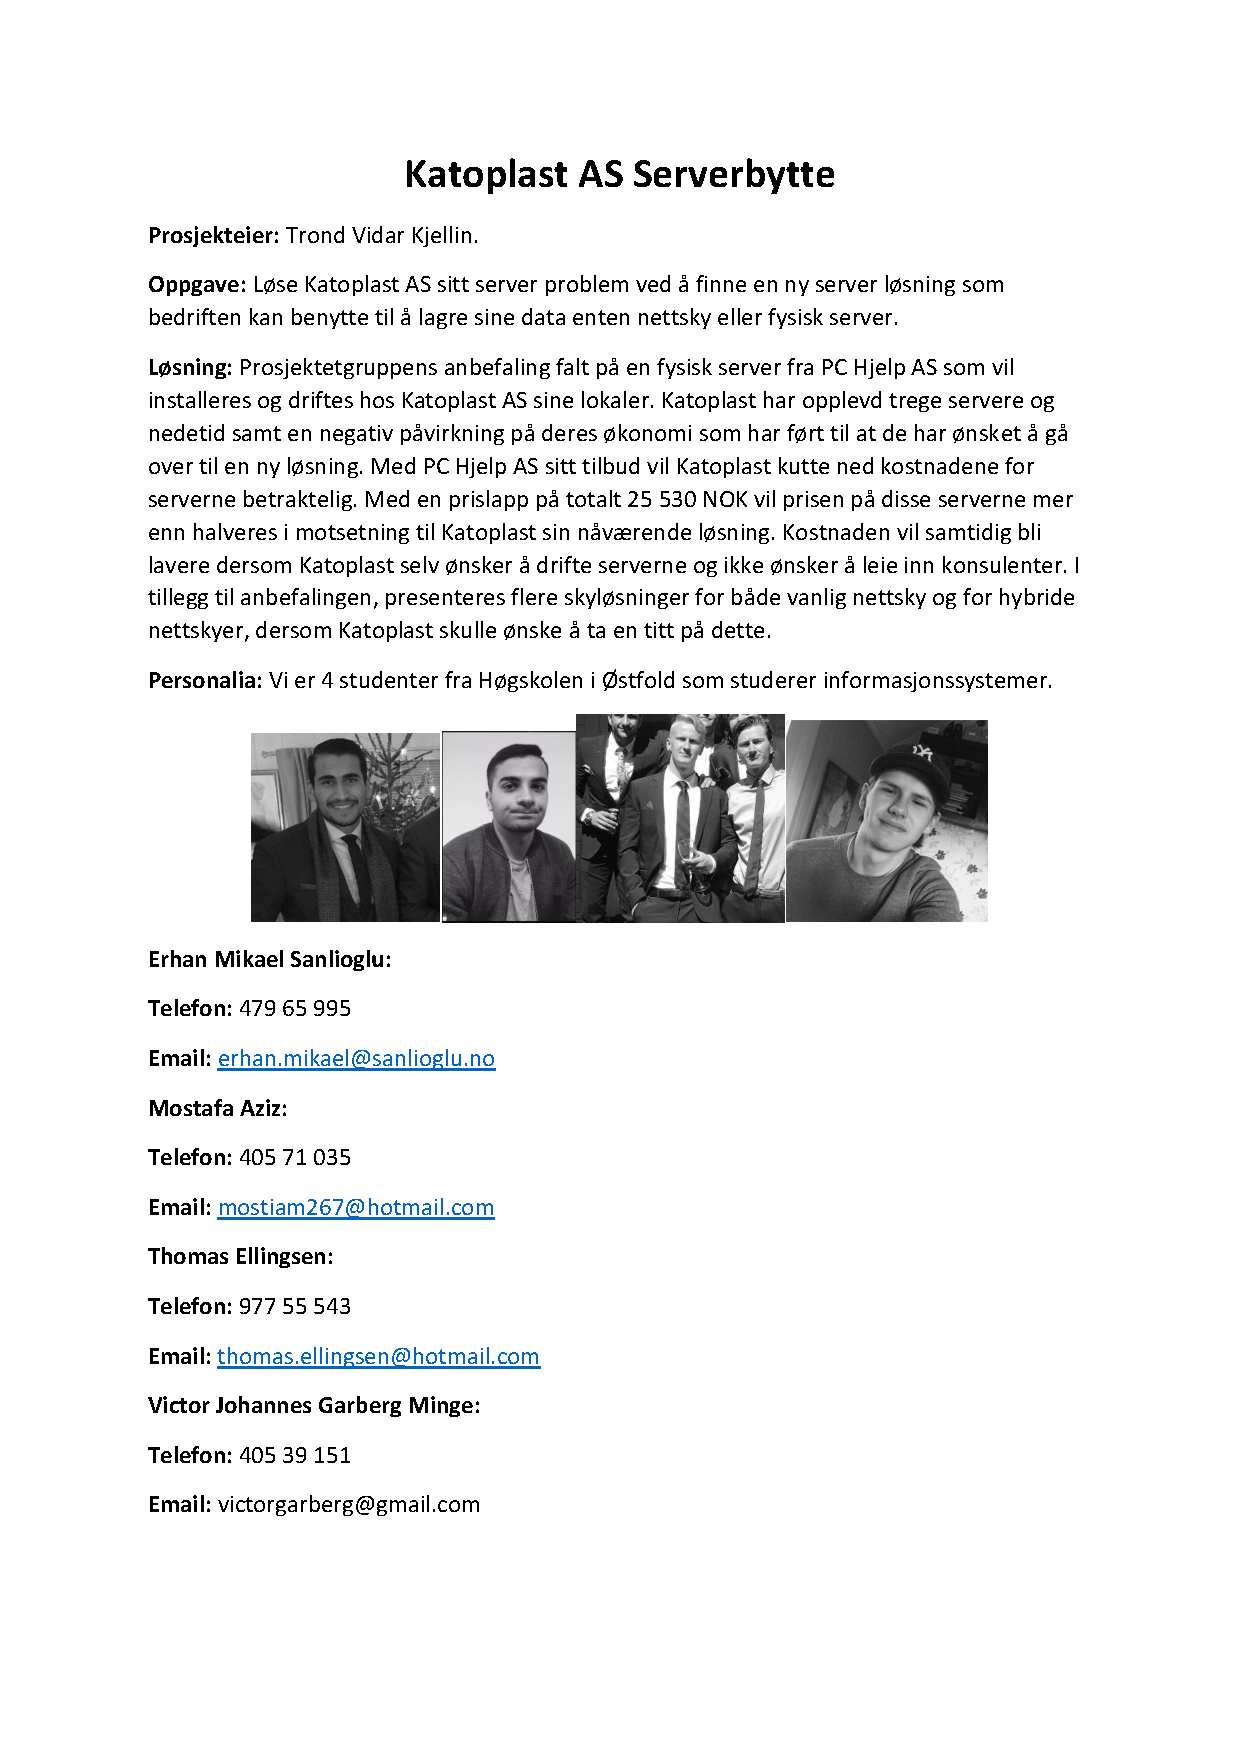
\includepdf[scale=1]{markedsf_ring.pdf}
%\include{Attachments/appendix}
% Include more appendices as required.
%%===================================
\end{document}